% Options for packages loaded elsewhere
\PassOptionsToPackage{unicode}{hyperref}
\PassOptionsToPackage{hyphens}{url}
%
\documentclass[
]{article}
\title{FAoptions}
\author{}
\date{\vspace{-2.5em}}

\usepackage{amsmath,amssymb}
\usepackage{lmodern}
\usepackage{iftex}
\ifPDFTeX
  \usepackage[T1]{fontenc}
  \usepackage[utf8]{inputenc}
  \usepackage{textcomp} % provide euro and other symbols
\else % if luatex or xetex
  \usepackage{unicode-math}
  \defaultfontfeatures{Scale=MatchLowercase}
  \defaultfontfeatures[\rmfamily]{Ligatures=TeX,Scale=1}
\fi
% Use upquote if available, for straight quotes in verbatim environments
\IfFileExists{upquote.sty}{\usepackage{upquote}}{}
\IfFileExists{microtype.sty}{% use microtype if available
  \usepackage[]{microtype}
  \UseMicrotypeSet[protrusion]{basicmath} % disable protrusion for tt fonts
}{}
\makeatletter
\@ifundefined{KOMAClassName}{% if non-KOMA class
  \IfFileExists{parskip.sty}{%
    \usepackage{parskip}
  }{% else
    \setlength{\parindent}{0pt}
    \setlength{\parskip}{6pt plus 2pt minus 1pt}}
}{% if KOMA class
  \KOMAoptions{parskip=half}}
\makeatother
\usepackage{xcolor}
\IfFileExists{xurl.sty}{\usepackage{xurl}}{} % add URL line breaks if available
\IfFileExists{bookmark.sty}{\usepackage{bookmark}}{\usepackage{hyperref}}
\hypersetup{
  pdftitle={FAoptions},
  hidelinks,
  pdfcreator={LaTeX via pandoc}}
\urlstyle{same} % disable monospaced font for URLs
\usepackage[margin=1in]{geometry}
\usepackage{graphicx}
\makeatletter
\def\maxwidth{\ifdim\Gin@nat@width>\linewidth\linewidth\else\Gin@nat@width\fi}
\def\maxheight{\ifdim\Gin@nat@height>\textheight\textheight\else\Gin@nat@height\fi}
\makeatother
% Scale images if necessary, so that they will not overflow the page
% margins by default, and it is still possible to overwrite the defaults
% using explicit options in \includegraphics[width, height, ...]{}
\setkeys{Gin}{width=\maxwidth,height=\maxheight,keepaspectratio}
% Set default figure placement to htbp
\makeatletter
\def\fps@figure{htbp}
\makeatother
\setlength{\emergencystretch}{3em} % prevent overfull lines
\providecommand{\tightlist}{%
  \setlength{\itemsep}{0pt}\setlength{\parskip}{0pt}}
\setcounter{secnumdepth}{-\maxdimen} % remove section numbering
\usepackage{pdflscape}
\newcommand{\blandscape}{\begin{landscape}}
\newcommand{\elandscape}{\end{landscape}}
\usepackage{booktabs}
\usepackage{longtable}
\usepackage{array}
\usepackage{multirow}
\usepackage{wrapfig}
\usepackage{float}
\usepackage{colortbl}
\usepackage{pdflscape}
\usepackage{tabu}
\usepackage{threeparttable}
\usepackage{threeparttablex}
\usepackage[normalem]{ulem}
\usepackage{makecell}
\usepackage{xcolor}
\usepackage{multicol}
\usepackage{hhline}
\newlength\Oldarrayrulewidth
\newlength\Oldtabcolsep
\usepackage{hyperref}
\ifLuaTeX
  \usepackage{selnolig}  % disable illegal ligatures
\fi

\begin{document}
\maketitle

{
\setcounter{tocdepth}{2}
\tableofcontents
}
\begin{landscape}

\hypertarget{fa-on-combined-scale-2-factor-solution-people-centered-development-and-nationalist-development}{%
\section{FA on Combined Scale (2 Factor Solution): People Centered
Development and Nationalist
Development}\label{fa-on-combined-scale-2-factor-solution-people-centered-development-and-nationalist-development}}

\hypertarget{nuclear-energy-efa-on-combined-scale-2-factor-solution}{%
\subsection{Nuclear Energy: EFA on Combined Scale (2 Factor
Solution)}\label{nuclear-energy-efa-on-combined-scale-2-factor-solution}}

\global\setlength{\Oldarrayrulewidth}{\arrayrulewidth}

\global\setlength{\Oldtabcolsep}{\tabcolsep}

\setlength{\tabcolsep}{0pt}

\renewcommand*{\arraystretch}{1.5}



\providecommand{\ascline}[3]{\noalign{\global\arrayrulewidth #1}\arrayrulecolor[HTML]{#2}\cline{#3}}

\begin{longtable}[c]{|p{1.50in}|p{4.50in}|p{0.75in}|p{0.75in}|p{0.75in}|p{0.75in}|p{0.75in}}

\caption{2\ factor\ solution}\\

\ascline{1.5pt}{666666}{1-7}

\multicolumn{1}{>{\raggedright}m{\dimexpr 1.5in+0\tabcolsep}}{\textcolor[HTML]{000000}{\fontsize{10}{10}\selectfont{code}}} & \multicolumn{1}{>{\raggedright}m{\dimexpr 4.5in+0\tabcolsep}}{\textcolor[HTML]{000000}{\fontsize{10}{10}\selectfont{Items}}} & \multicolumn{1}{>{\raggedright}m{\dimexpr 0.75in+0\tabcolsep}}{\textcolor[HTML]{000000}{\fontsize{10}{10}\selectfont{Pdevelop}}} & \multicolumn{1}{>{\raggedright}m{\dimexpr 0.75in+0\tabcolsep}}{\textcolor[HTML]{000000}{\fontsize{10}{10}\selectfont{Ndevelop}}} & \multicolumn{1}{>{\raggedleft}m{\dimexpr 0.75in+0\tabcolsep}}{\textcolor[HTML]{000000}{\fontsize{10}{10}\selectfont{Communality}}} & \multicolumn{1}{>{\raggedleft}m{\dimexpr 0.75in+0\tabcolsep}}{\textcolor[HTML]{000000}{\fontsize{10}{10}\selectfont{Uniqueness}}} & \multicolumn{1}{>{\raggedleft}m{\dimexpr 0.75in+0\tabcolsep}}{\textcolor[HTML]{000000}{\fontsize{10}{10}\selectfont{Complexity}}} \\

\ascline{1.5pt}{666666}{1-7}\endfirsthead \caption[]{2\ factor\ solution}\\

\ascline{1.5pt}{666666}{1-7}

\multicolumn{1}{>{\raggedright}m{\dimexpr 1.5in+0\tabcolsep}}{\textcolor[HTML]{000000}{\fontsize{10}{10}\selectfont{code}}} & \multicolumn{1}{>{\raggedright}m{\dimexpr 4.5in+0\tabcolsep}}{\textcolor[HTML]{000000}{\fontsize{10}{10}\selectfont{Items}}} & \multicolumn{1}{>{\raggedright}m{\dimexpr 0.75in+0\tabcolsep}}{\textcolor[HTML]{000000}{\fontsize{10}{10}\selectfont{Pdevelop}}} & \multicolumn{1}{>{\raggedright}m{\dimexpr 0.75in+0\tabcolsep}}{\textcolor[HTML]{000000}{\fontsize{10}{10}\selectfont{Ndevelop}}} & \multicolumn{1}{>{\raggedleft}m{\dimexpr 0.75in+0\tabcolsep}}{\textcolor[HTML]{000000}{\fontsize{10}{10}\selectfont{Communality}}} & \multicolumn{1}{>{\raggedleft}m{\dimexpr 0.75in+0\tabcolsep}}{\textcolor[HTML]{000000}{\fontsize{10}{10}\selectfont{Uniqueness}}} & \multicolumn{1}{>{\raggedleft}m{\dimexpr 0.75in+0\tabcolsep}}{\textcolor[HTML]{000000}{\fontsize{10}{10}\selectfont{Complexity}}} \\

\ascline{1.5pt}{666666}{1-7}\endhead



\multicolumn{1}{>{\raggedright}m{\dimexpr 1.5in+0\tabcolsep}}{\textcolor[HTML]{000000}{\fontsize{10}{10}\selectfont{Health\ risk(nuclear)}}} & \multicolumn{1}{>{\raggedright}m{\dimexpr 4.5in+0\tabcolsep}}{\textcolor[HTML]{000000}{\fontsize{10}{10}\selectfont{Nuclear\ energy\ poses\ a\ great\ risk\ to\ the\ health\ of\ people\ living\ around\ it}}} & \multicolumn{1}{>{\raggedright}m{\dimexpr 0.75in+0\tabcolsep}}{\textcolor[HTML]{000000}{\fontsize{10}{10}\selectfont{0.663}}} & \multicolumn{1}{>{\raggedright}m{\dimexpr 0.75in+0\tabcolsep}}{\textcolor[HTML]{000000}{\fontsize{10}{10}\selectfont{}}} & \multicolumn{1}{>{\raggedleft}m{\dimexpr 0.75in+0\tabcolsep}}{\textcolor[HTML]{000000}{\fontsize{10}{10}\selectfont{0.447}}} & \multicolumn{1}{>{\raggedleft}m{\dimexpr 0.75in+0\tabcolsep}}{\textcolor[HTML]{000000}{\fontsize{10}{10}\selectfont{0.553}}} & \multicolumn{1}{>{\raggedleft}m{\dimexpr 0.75in+0\tabcolsep}}{\textcolor[HTML]{000000}{\fontsize{10}{10}\selectfont{1.034}}} \\





\multicolumn{1}{>{\raggedright}m{\dimexpr 1.5in+0\tabcolsep}}{\textcolor[HTML]{000000}{\fontsize{10}{10}\selectfont{Spoils\ Natural\ Beauty(nuclear)}}} & \multicolumn{1}{>{\raggedright}m{\dimexpr 4.5in+0\tabcolsep}}{\textcolor[HTML]{000000}{\fontsize{10}{10}\selectfont{Nuclear\ energy\ spoils\ the\ natural\ beauty\ of\ the\ landscape}}} & \multicolumn{1}{>{\raggedright}m{\dimexpr 0.75in+0\tabcolsep}}{\textcolor[HTML]{000000}{\fontsize{10}{10}\selectfont{0.619}}} & \multicolumn{1}{>{\raggedright}m{\dimexpr 0.75in+0\tabcolsep}}{\textcolor[HTML]{000000}{\fontsize{10}{10}\selectfont{}}} & \multicolumn{1}{>{\raggedleft}m{\dimexpr 0.75in+0\tabcolsep}}{\textcolor[HTML]{000000}{\fontsize{10}{10}\selectfont{0.390}}} & \multicolumn{1}{>{\raggedleft}m{\dimexpr 0.75in+0\tabcolsep}}{\textcolor[HTML]{000000}{\fontsize{10}{10}\selectfont{0.610}}} & \multicolumn{1}{>{\raggedleft}m{\dimexpr 0.75in+0\tabcolsep}}{\textcolor[HTML]{000000}{\fontsize{10}{10}\selectfont{1.035}}} \\





\multicolumn{1}{>{\raggedright}m{\dimexpr 1.5in+0\tabcolsep}}{\textcolor[HTML]{000000}{\fontsize{10}{10}\selectfont{Pollution\ risk(nuclear)}}} & \multicolumn{1}{>{\raggedright}m{\dimexpr 4.5in+0\tabcolsep}}{\textcolor[HTML]{000000}{\fontsize{10}{10}\selectfont{Nuclear\ energy\ increases\ pollution\ of\ air/water/land}}} & \multicolumn{1}{>{\raggedright}m{\dimexpr 0.75in+0\tabcolsep}}{\textcolor[HTML]{000000}{\fontsize{10}{10}\selectfont{0.578}}} & \multicolumn{1}{>{\raggedright}m{\dimexpr 0.75in+0\tabcolsep}}{\textcolor[HTML]{000000}{\fontsize{10}{10}\selectfont{}}} & \multicolumn{1}{>{\raggedleft}m{\dimexpr 0.75in+0\tabcolsep}}{\textcolor[HTML]{000000}{\fontsize{10}{10}\selectfont{0.335}}} & \multicolumn{1}{>{\raggedleft}m{\dimexpr 0.75in+0\tabcolsep}}{\textcolor[HTML]{000000}{\fontsize{10}{10}\selectfont{0.665}}} & \multicolumn{1}{>{\raggedleft}m{\dimexpr 0.75in+0\tabcolsep}}{\textcolor[HTML]{000000}{\fontsize{10}{10}\selectfont{1.002}}} \\





\multicolumn{1}{>{\raggedright}m{\dimexpr 1.5in+0\tabcolsep}}{\textcolor[HTML]{000000}{\fontsize{10}{10}\selectfont{Displacement\ risk(nuclear)}}} & \multicolumn{1}{>{\raggedright}m{\dimexpr 4.5in+0\tabcolsep}}{\textcolor[HTML]{000000}{\fontsize{10}{10}\selectfont{Nuclear\ energy\ is\ leading\ to\ displacement\ of\ people\ from\ their\ land}}} & \multicolumn{1}{>{\raggedright}m{\dimexpr 0.75in+0\tabcolsep}}{\textcolor[HTML]{000000}{\fontsize{10}{10}\selectfont{0.574}}} & \multicolumn{1}{>{\raggedright}m{\dimexpr 0.75in+0\tabcolsep}}{\textcolor[HTML]{000000}{\fontsize{10}{10}\selectfont{}}} & \multicolumn{1}{>{\raggedleft}m{\dimexpr 0.75in+0\tabcolsep}}{\textcolor[HTML]{000000}{\fontsize{10}{10}\selectfont{0.371}}} & \multicolumn{1}{>{\raggedleft}m{\dimexpr 0.75in+0\tabcolsep}}{\textcolor[HTML]{000000}{\fontsize{10}{10}\selectfont{0.629}}} & \multicolumn{1}{>{\raggedleft}m{\dimexpr 0.75in+0\tabcolsep}}{\textcolor[HTML]{000000}{\fontsize{10}{10}\selectfont{1.249}}} \\





\multicolumn{1}{>{\raggedright}m{\dimexpr 1.5in+0\tabcolsep}}{\textcolor[HTML]{000000}{\fontsize{10}{10}\selectfont{Anti\ Mechanisation\ of\ work}}} & \multicolumn{1}{>{\raggedright}m{\dimexpr 4.5in+0\tabcolsep}}{\textcolor[HTML]{000000}{\fontsize{10}{10}\selectfont{Rapid\ mechanization\ of\ work\ is\ taking\ away\ jobs\ from\ workers\ in\ this\ country}}} & \multicolumn{1}{>{\raggedright}m{\dimexpr 0.75in+0\tabcolsep}}{\textcolor[HTML]{000000}{\fontsize{10}{10}\selectfont{0.54}}} & \multicolumn{1}{>{\raggedright}m{\dimexpr 0.75in+0\tabcolsep}}{\textcolor[HTML]{000000}{\fontsize{10}{10}\selectfont{}}} & \multicolumn{1}{>{\raggedleft}m{\dimexpr 0.75in+0\tabcolsep}}{\textcolor[HTML]{000000}{\fontsize{10}{10}\selectfont{0.336}}} & \multicolumn{1}{>{\raggedleft}m{\dimexpr 0.75in+0\tabcolsep}}{\textcolor[HTML]{000000}{\fontsize{10}{10}\selectfont{0.664}}} & \multicolumn{1}{>{\raggedleft}m{\dimexpr 0.75in+0\tabcolsep}}{\textcolor[HTML]{000000}{\fontsize{10}{10}\selectfont{1.297}}} \\





\multicolumn{1}{>{\raggedright}m{\dimexpr 1.5in+0\tabcolsep}}{\textcolor[HTML]{000000}{\fontsize{10}{10}\selectfont{Pro\ Regulations}}} & \multicolumn{1}{>{\raggedright}m{\dimexpr 4.5in+0\tabcolsep}}{\textcolor[HTML]{000000}{\fontsize{10}{10}\selectfont{Regardless\ of\ ownership,\ the\ government\ should\ pass\ strong\ regulations\ and\ implement\ them}}} & \multicolumn{1}{>{\raggedright}m{\dimexpr 0.75in+0\tabcolsep}}{\textcolor[HTML]{000000}{\fontsize{10}{10}\selectfont{0.534}}} & \multicolumn{1}{>{\raggedright}m{\dimexpr 0.75in+0\tabcolsep}}{\textcolor[HTML]{000000}{\fontsize{10}{10}\selectfont{}}} & \multicolumn{1}{>{\raggedleft}m{\dimexpr 0.75in+0\tabcolsep}}{\textcolor[HTML]{000000}{\fontsize{10}{10}\selectfont{0.301}}} & \multicolumn{1}{>{\raggedleft}m{\dimexpr 0.75in+0\tabcolsep}}{\textcolor[HTML]{000000}{\fontsize{10}{10}\selectfont{0.699}}} & \multicolumn{1}{>{\raggedleft}m{\dimexpr 0.75in+0\tabcolsep}}{\textcolor[HTML]{000000}{\fontsize{10}{10}\selectfont{1.116}}} \\





\multicolumn{1}{>{\raggedright}m{\dimexpr 1.5in+0\tabcolsep}}{\textcolor[HTML]{000000}{\fontsize{10}{10}\selectfont{Anti\ Large\ Industries}}} & \multicolumn{1}{>{\raggedright}m{\dimexpr 4.5in+0\tabcolsep}}{\textcolor[HTML]{000000}{\fontsize{10}{10}\selectfont{Large\ corporations\ are\ destroying\ the\ local\ industries\ in\ India\ and\ benefiting\ only\ a\ handful\ of\ people}}} & \multicolumn{1}{>{\raggedright}m{\dimexpr 0.75in+0\tabcolsep}}{\textcolor[HTML]{000000}{\fontsize{10}{10}\selectfont{0.523}}} & \multicolumn{1}{>{\raggedright}m{\dimexpr 0.75in+0\tabcolsep}}{\textcolor[HTML]{000000}{\fontsize{10}{10}\selectfont{}}} & \multicolumn{1}{>{\raggedleft}m{\dimexpr 0.75in+0\tabcolsep}}{\textcolor[HTML]{000000}{\fontsize{10}{10}\selectfont{0.275}}} & \multicolumn{1}{>{\raggedleft}m{\dimexpr 0.75in+0\tabcolsep}}{\textcolor[HTML]{000000}{\fontsize{10}{10}\selectfont{0.725}}} & \multicolumn{1}{>{\raggedleft}m{\dimexpr 0.75in+0\tabcolsep}}{\textcolor[HTML]{000000}{\fontsize{10}{10}\selectfont{1.014}}} \\





\multicolumn{1}{>{\raggedright}m{\dimexpr 1.5in+0\tabcolsep}}{\textcolor[HTML]{000000}{\fontsize{10}{10}\selectfont{Environment\ over\ Development}}} & \multicolumn{1}{>{\raggedright}m{\dimexpr 4.5in+0\tabcolsep}}{\textcolor[HTML]{000000}{\fontsize{10}{10}\selectfont{Polluting\ industries\ that\ spoil\ the\ environment\ should\ be\ shut\ down\ even\ if\ it\ costs\ people\ their\ jobs}}} & \multicolumn{1}{>{\raggedright}m{\dimexpr 0.75in+0\tabcolsep}}{\textcolor[HTML]{000000}{\fontsize{10}{10}\selectfont{0.417}}} & \multicolumn{1}{>{\raggedright}m{\dimexpr 0.75in+0\tabcolsep}}{\textcolor[HTML]{000000}{\fontsize{10}{10}\selectfont{}}} & \multicolumn{1}{>{\raggedleft}m{\dimexpr 0.75in+0\tabcolsep}}{\textcolor[HTML]{000000}{\fontsize{10}{10}\selectfont{0.175}}} & \multicolumn{1}{>{\raggedleft}m{\dimexpr 0.75in+0\tabcolsep}}{\textcolor[HTML]{000000}{\fontsize{10}{10}\selectfont{0.825}}} & \multicolumn{1}{>{\raggedleft}m{\dimexpr 0.75in+0\tabcolsep}}{\textcolor[HTML]{000000}{\fontsize{10}{10}\selectfont{1.011}}} \\





\multicolumn{1}{>{\raggedright}m{\dimexpr 1.5in+0\tabcolsep}}{\textcolor[HTML]{000000}{\fontsize{10}{10}\selectfont{Pro\ Public\ ownership}}} & \multicolumn{1}{>{\raggedright}m{\dimexpr 4.5in+0\tabcolsep}}{\textcolor[HTML]{000000}{\fontsize{10}{10}\selectfont{The\ government\ should\ own\ most\ large\ businesses\ and\ industries}}} & \multicolumn{1}{>{\raggedright}m{\dimexpr 0.75in+0\tabcolsep}}{\textcolor[HTML]{000000}{\fontsize{10}{10}\selectfont{}}} & \multicolumn{1}{>{\raggedright}m{\dimexpr 0.75in+0\tabcolsep}}{\textcolor[HTML]{000000}{\fontsize{10}{10}\selectfont{}}} & \multicolumn{1}{>{\raggedleft}m{\dimexpr 0.75in+0\tabcolsep}}{\textcolor[HTML]{000000}{\fontsize{10}{10}\selectfont{0.140}}} & \multicolumn{1}{>{\raggedleft}m{\dimexpr 0.75in+0\tabcolsep}}{\textcolor[HTML]{000000}{\fontsize{10}{10}\selectfont{0.860}}} & \multicolumn{1}{>{\raggedleft}m{\dimexpr 0.75in+0\tabcolsep}}{\textcolor[HTML]{000000}{\fontsize{10}{10}\selectfont{1.218}}} \\





\multicolumn{1}{>{\raggedright}m{\dimexpr 1.5in+0\tabcolsep}}{\textcolor[HTML]{000000}{\fontsize{10}{10}\selectfont{Pro\ Globaleconomy}}} & \multicolumn{1}{>{\raggedright}m{\dimexpr 4.5in+0\tabcolsep}}{\textcolor[HTML]{000000}{\fontsize{10}{10}\selectfont{Foreign\ companies\ have\ led\ to\ a\ range\ of\ benefits\ for\ the\ Indian\ people\ and\ society}}} & \multicolumn{1}{>{\raggedright}m{\dimexpr 0.75in+0\tabcolsep}}{\textcolor[HTML]{000000}{\fontsize{10}{10}\selectfont{}}} & \multicolumn{1}{>{\raggedright}m{\dimexpr 0.75in+0\tabcolsep}}{\textcolor[HTML]{000000}{\fontsize{10}{10}\selectfont{}}} & \multicolumn{1}{>{\raggedleft}m{\dimexpr 0.75in+0\tabcolsep}}{\textcolor[HTML]{000000}{\fontsize{10}{10}\selectfont{0.227}}} & \multicolumn{1}{>{\raggedleft}m{\dimexpr 0.75in+0\tabcolsep}}{\textcolor[HTML]{000000}{\fontsize{10}{10}\selectfont{0.773}}} & \multicolumn{1}{>{\raggedleft}m{\dimexpr 0.75in+0\tabcolsep}}{\textcolor[HTML]{000000}{\fontsize{10}{10}\selectfont{1.997}}} \\





\multicolumn{1}{>{\raggedright}m{\dimexpr 1.5in+0\tabcolsep}}{\textcolor[HTML]{000000}{\fontsize{10}{10}\selectfont{Pro\ Decentralisation}}} & \multicolumn{1}{>{\raggedright}m{\dimexpr 4.5in+0\tabcolsep}}{\textcolor[HTML]{000000}{\fontsize{10}{10}\selectfont{Local\ politicians\ shouldn't\ have\ to\ ask\ permission\ from\ the\ central\ government\ to\ implement\ policies}}} & \multicolumn{1}{>{\raggedright}m{\dimexpr 0.75in+0\tabcolsep}}{\textcolor[HTML]{000000}{\fontsize{10}{10}\selectfont{}}} & \multicolumn{1}{>{\raggedright}m{\dimexpr 0.75in+0\tabcolsep}}{\textcolor[HTML]{000000}{\fontsize{10}{10}\selectfont{}}} & \multicolumn{1}{>{\raggedleft}m{\dimexpr 0.75in+0\tabcolsep}}{\textcolor[HTML]{000000}{\fontsize{10}{10}\selectfont{0.102}}} & \multicolumn{1}{>{\raggedleft}m{\dimexpr 0.75in+0\tabcolsep}}{\textcolor[HTML]{000000}{\fontsize{10}{10}\selectfont{0.898}}} & \multicolumn{1}{>{\raggedleft}m{\dimexpr 0.75in+0\tabcolsep}}{\textcolor[HTML]{000000}{\fontsize{10}{10}\selectfont{1.001}}} \\





\multicolumn{1}{>{\raggedright}m{\dimexpr 1.5in+0\tabcolsep}}{\textcolor[HTML]{000000}{\fontsize{10}{10}\selectfont{Limits\ on\ Wealth}}} & \multicolumn{1}{>{\raggedright}m{\dimexpr 4.5in+0\tabcolsep}}{\textcolor[HTML]{000000}{\fontsize{10}{10}\selectfont{A\ limit\ should\ be\ put\ to\ how\ much\ wealth\ a\ person\ can\ amass}}} & \multicolumn{1}{>{\raggedright}m{\dimexpr 0.75in+0\tabcolsep}}{\textcolor[HTML]{000000}{\fontsize{10}{10}\selectfont{}}} & \multicolumn{1}{>{\raggedright}m{\dimexpr 0.75in+0\tabcolsep}}{\textcolor[HTML]{000000}{\fontsize{10}{10}\selectfont{}}} & \multicolumn{1}{>{\raggedleft}m{\dimexpr 0.75in+0\tabcolsep}}{\textcolor[HTML]{000000}{\fontsize{10}{10}\selectfont{0.153}}} & \multicolumn{1}{>{\raggedleft}m{\dimexpr 0.75in+0\tabcolsep}}{\textcolor[HTML]{000000}{\fontsize{10}{10}\selectfont{0.847}}} & \multicolumn{1}{>{\raggedleft}m{\dimexpr 0.75in+0\tabcolsep}}{\textcolor[HTML]{000000}{\fontsize{10}{10}\selectfont{2.000}}} \\





\multicolumn{1}{>{\raggedright}m{\dimexpr 1.5in+0\tabcolsep}}{\textcolor[HTML]{000000}{\fontsize{10}{10}\selectfont{Pro\ Private\ ownership}}} & \multicolumn{1}{>{\raggedright}m{\dimexpr 4.5in+0\tabcolsep}}{\textcolor[HTML]{000000}{\fontsize{10}{10}\selectfont{All\ businesses\ and\ industries\ should\ be\ owned\ privately}}} & \multicolumn{1}{>{\raggedright}m{\dimexpr 0.75in+0\tabcolsep}}{\textcolor[HTML]{000000}{\fontsize{10}{10}\selectfont{}}} & \multicolumn{1}{>{\raggedright}m{\dimexpr 0.75in+0\tabcolsep}}{\textcolor[HTML]{000000}{\fontsize{10}{10}\selectfont{}}} & \multicolumn{1}{>{\raggedleft}m{\dimexpr 0.75in+0\tabcolsep}}{\textcolor[HTML]{000000}{\fontsize{10}{10}\selectfont{0.042}}} & \multicolumn{1}{>{\raggedleft}m{\dimexpr 0.75in+0\tabcolsep}}{\textcolor[HTML]{000000}{\fontsize{10}{10}\selectfont{0.958}}} & \multicolumn{1}{>{\raggedleft}m{\dimexpr 0.75in+0\tabcolsep}}{\textcolor[HTML]{000000}{\fontsize{10}{10}\selectfont{1.757}}} \\





\multicolumn{1}{>{\raggedright}m{\dimexpr 1.5in+0\tabcolsep}}{\textcolor[HTML]{000000}{\fontsize{10}{10}\selectfont{Pro\ Localeconomy}}} & \multicolumn{1}{>{\raggedright}m{\dimexpr 4.5in+0\tabcolsep}}{\textcolor[HTML]{000000}{\fontsize{10}{10}\selectfont{India\ would\ be\ better\ off\ if\ foreign\ companies\ didn't\ come\ to\ here}}} & \multicolumn{1}{>{\raggedright}m{\dimexpr 0.75in+0\tabcolsep}}{\textcolor[HTML]{000000}{\fontsize{10}{10}\selectfont{}}} & \multicolumn{1}{>{\raggedright}m{\dimexpr 0.75in+0\tabcolsep}}{\textcolor[HTML]{000000}{\fontsize{10}{10}\selectfont{}}} & \multicolumn{1}{>{\raggedleft}m{\dimexpr 0.75in+0\tabcolsep}}{\textcolor[HTML]{000000}{\fontsize{10}{10}\selectfont{0.017}}} & \multicolumn{1}{>{\raggedleft}m{\dimexpr 0.75in+0\tabcolsep}}{\textcolor[HTML]{000000}{\fontsize{10}{10}\selectfont{0.983}}} & \multicolumn{1}{>{\raggedleft}m{\dimexpr 0.75in+0\tabcolsep}}{\textcolor[HTML]{000000}{\fontsize{10}{10}\selectfont{1.057}}} \\





\multicolumn{1}{>{\raggedright}m{\dimexpr 1.5in+0\tabcolsep}}{\textcolor[HTML]{000000}{\fontsize{10}{10}\selectfont{National\ development(nuclear)}}} & \multicolumn{1}{>{\raggedright}m{\dimexpr 4.5in+0\tabcolsep}}{\textcolor[HTML]{000000}{\fontsize{10}{10}\selectfont{Nuclear\ energy\ pushes\ forward\ the\ country's\ development}}} & \multicolumn{1}{>{\raggedright}m{\dimexpr 0.75in+0\tabcolsep}}{\textcolor[HTML]{000000}{\fontsize{10}{10}\selectfont{}}} & \multicolumn{1}{>{\raggedright}m{\dimexpr 0.75in+0\tabcolsep}}{\textcolor[HTML]{000000}{\fontsize{10}{10}\selectfont{0.665}}} & \multicolumn{1}{>{\raggedleft}m{\dimexpr 0.75in+0\tabcolsep}}{\textcolor[HTML]{000000}{\fontsize{10}{10}\selectfont{0.464}}} & \multicolumn{1}{>{\raggedleft}m{\dimexpr 0.75in+0\tabcolsep}}{\textcolor[HTML]{000000}{\fontsize{10}{10}\selectfont{0.536}}} & \multicolumn{1}{>{\raggedleft}m{\dimexpr 0.75in+0\tabcolsep}}{\textcolor[HTML]{000000}{\fontsize{10}{10}\selectfont{1.095}}} \\





\multicolumn{1}{>{\raggedright}m{\dimexpr 1.5in+0\tabcolsep}}{\textcolor[HTML]{000000}{\fontsize{10}{10}\selectfont{Community\ pride(nuclear)}}} & \multicolumn{1}{>{\raggedright}m{\dimexpr 4.5in+0\tabcolsep}}{\textcolor[HTML]{000000}{\fontsize{10}{10}\selectfont{I\ would\ be\ proud\ if\ my\ community\ used\ nuclear\ energy}}} & \multicolumn{1}{>{\raggedright}m{\dimexpr 0.75in+0\tabcolsep}}{\textcolor[HTML]{000000}{\fontsize{10}{10}\selectfont{}}} & \multicolumn{1}{>{\raggedright}m{\dimexpr 0.75in+0\tabcolsep}}{\textcolor[HTML]{000000}{\fontsize{10}{10}\selectfont{0.622}}} & \multicolumn{1}{>{\raggedleft}m{\dimexpr 0.75in+0\tabcolsep}}{\textcolor[HTML]{000000}{\fontsize{10}{10}\selectfont{0.450}}} & \multicolumn{1}{>{\raggedleft}m{\dimexpr 0.75in+0\tabcolsep}}{\textcolor[HTML]{000000}{\fontsize{10}{10}\selectfont{0.550}}} & \multicolumn{1}{>{\raggedleft}m{\dimexpr 0.75in+0\tabcolsep}}{\textcolor[HTML]{000000}{\fontsize{10}{10}\selectfont{1.321}}} \\





\multicolumn{1}{>{\raggedright}m{\dimexpr 1.5in+0\tabcolsep}}{\textcolor[HTML]{000000}{\fontsize{10}{10}\selectfont{National\ pride(nuclear)}}} & \multicolumn{1}{>{\raggedright}m{\dimexpr 4.5in+0\tabcolsep}}{\textcolor[HTML]{000000}{\fontsize{10}{10}\selectfont{Nuclear\ energy\ is\ a\ mark\ of\ pride\ for\ our\ nation}}} & \multicolumn{1}{>{\raggedright}m{\dimexpr 0.75in+0\tabcolsep}}{\textcolor[HTML]{000000}{\fontsize{10}{10}\selectfont{}}} & \multicolumn{1}{>{\raggedright}m{\dimexpr 0.75in+0\tabcolsep}}{\textcolor[HTML]{000000}{\fontsize{10}{10}\selectfont{0.597}}} & \multicolumn{1}{>{\raggedleft}m{\dimexpr 0.75in+0\tabcolsep}}{\textcolor[HTML]{000000}{\fontsize{10}{10}\selectfont{0.405}}} & \multicolumn{1}{>{\raggedleft}m{\dimexpr 0.75in+0\tabcolsep}}{\textcolor[HTML]{000000}{\fontsize{10}{10}\selectfont{0.595}}} & \multicolumn{1}{>{\raggedleft}m{\dimexpr 0.75in+0\tabcolsep}}{\textcolor[HTML]{000000}{\fontsize{10}{10}\selectfont{1.266}}} \\





\multicolumn{1}{>{\raggedright}m{\dimexpr 1.5in+0\tabcolsep}}{\textcolor[HTML]{000000}{\fontsize{10}{10}\selectfont{Local\ prosperity(nuclear)}}} & \multicolumn{1}{>{\raggedright}m{\dimexpr 4.5in+0\tabcolsep}}{\textcolor[HTML]{000000}{\fontsize{10}{10}\selectfont{Nuclear\ energy\ brings\ economic\ prosperity\ to\ the\ surrounding\ regions}}} & \multicolumn{1}{>{\raggedright}m{\dimexpr 0.75in+0\tabcolsep}}{\textcolor[HTML]{000000}{\fontsize{10}{10}\selectfont{}}} & \multicolumn{1}{>{\raggedright}m{\dimexpr 0.75in+0\tabcolsep}}{\textcolor[HTML]{000000}{\fontsize{10}{10}\selectfont{0.594}}} & \multicolumn{1}{>{\raggedleft}m{\dimexpr 0.75in+0\tabcolsep}}{\textcolor[HTML]{000000}{\fontsize{10}{10}\selectfont{0.363}}} & \multicolumn{1}{>{\raggedleft}m{\dimexpr 0.75in+0\tabcolsep}}{\textcolor[HTML]{000000}{\fontsize{10}{10}\selectfont{0.637}}} & \multicolumn{1}{>{\raggedleft}m{\dimexpr 0.75in+0\tabcolsep}}{\textcolor[HTML]{000000}{\fontsize{10}{10}\selectfont{1.055}}} \\





\multicolumn{1}{>{\raggedright}m{\dimexpr 1.5in+0\tabcolsep}}{\textcolor[HTML]{000000}{\fontsize{10}{10}\selectfont{Job\ opportunities(nuclear)}}} & \multicolumn{1}{>{\raggedright}m{\dimexpr 4.5in+0\tabcolsep}}{\textcolor[HTML]{000000}{\fontsize{10}{10}\selectfont{Nuclear\ energy\ will\ bring\ jobs\ to\ the\ local\ community}}} & \multicolumn{1}{>{\raggedright}m{\dimexpr 0.75in+0\tabcolsep}}{\textcolor[HTML]{000000}{\fontsize{10}{10}\selectfont{}}} & \multicolumn{1}{>{\raggedright}m{\dimexpr 0.75in+0\tabcolsep}}{\textcolor[HTML]{000000}{\fontsize{10}{10}\selectfont{0.428}}} & \multicolumn{1}{>{\raggedleft}m{\dimexpr 0.75in+0\tabcolsep}}{\textcolor[HTML]{000000}{\fontsize{10}{10}\selectfont{0.223}}} & \multicolumn{1}{>{\raggedleft}m{\dimexpr 0.75in+0\tabcolsep}}{\textcolor[HTML]{000000}{\fontsize{10}{10}\selectfont{0.777}}} & \multicolumn{1}{>{\raggedleft}m{\dimexpr 0.75in+0\tabcolsep}}{\textcolor[HTML]{000000}{\fontsize{10}{10}\selectfont{1.409}}} \\





\multicolumn{1}{>{\raggedright}m{\dimexpr 1.5in+0\tabcolsep}}{\textcolor[HTML]{000000}{\fontsize{10}{10}\selectfont{Reliance\ on\ government(nuclear)}}} & \multicolumn{1}{>{\raggedright}m{\dimexpr 4.5in+0\tabcolsep}}{\textcolor[HTML]{000000}{\fontsize{10}{10}\selectfont{I\ don't\ like\ the\ idea\ that\ I\ have\ to\ rely\ on\ the\ government\ for\ electricity\ from\ nuclear\ energy}}} & \multicolumn{1}{>{\raggedright}m{\dimexpr 0.75in+0\tabcolsep}}{\textcolor[HTML]{000000}{\fontsize{10}{10}\selectfont{}}} & \multicolumn{1}{>{\raggedright}m{\dimexpr 0.75in+0\tabcolsep}}{\textcolor[HTML]{000000}{\fontsize{10}{10}\selectfont{}}} & \multicolumn{1}{>{\raggedleft}m{\dimexpr 0.75in+0\tabcolsep}}{\textcolor[HTML]{000000}{\fontsize{10}{10}\selectfont{0.156}}} & \multicolumn{1}{>{\raggedleft}m{\dimexpr 0.75in+0\tabcolsep}}{\textcolor[HTML]{000000}{\fontsize{10}{10}\selectfont{0.844}}} & \multicolumn{1}{>{\raggedleft}m{\dimexpr 0.75in+0\tabcolsep}}{\textcolor[HTML]{000000}{\fontsize{10}{10}\selectfont{1.005}}} \\





\multicolumn{1}{>{\raggedright}m{\dimexpr 1.5in+0\tabcolsep}}{\textcolor[HTML]{000000}{\fontsize{10}{10}\selectfont{Pro\ Large\ Industries}}} & \multicolumn{1}{>{\raggedright}m{\dimexpr 4.5in+0\tabcolsep}}{\textcolor[HTML]{000000}{\fontsize{10}{10}\selectfont{Large\ scale\ industries\ are\ required\ for\ the\ development\ of\ the\ country\ that\ will\ benefit\ everyone}}} & \multicolumn{1}{>{\raggedright}m{\dimexpr 0.75in+0\tabcolsep}}{\textcolor[HTML]{000000}{\fontsize{10}{10}\selectfont{}}} & \multicolumn{1}{>{\raggedright}m{\dimexpr 0.75in+0\tabcolsep}}{\textcolor[HTML]{000000}{\fontsize{10}{10}\selectfont{}}} & \multicolumn{1}{>{\raggedleft}m{\dimexpr 0.75in+0\tabcolsep}}{\textcolor[HTML]{000000}{\fontsize{10}{10}\selectfont{0.170}}} & \multicolumn{1}{>{\raggedleft}m{\dimexpr 0.75in+0\tabcolsep}}{\textcolor[HTML]{000000}{\fontsize{10}{10}\selectfont{0.830}}} & \multicolumn{1}{>{\raggedleft}m{\dimexpr 0.75in+0\tabcolsep}}{\textcolor[HTML]{000000}{\fontsize{10}{10}\selectfont{1.712}}} \\





\multicolumn{1}{>{\raggedright}m{\dimexpr 1.5in+0\tabcolsep}}{\textcolor[HTML]{000000}{\fontsize{10}{10}\selectfont{Pro\ Centralisation}}} & \multicolumn{1}{>{\raggedright}m{\dimexpr 4.5in+0\tabcolsep}}{\textcolor[HTML]{000000}{\fontsize{10}{10}\selectfont{Laws\ and\ policies\ would\ be\ implemented\ more\ smoothly\ if\ more\ power\ lay\ with\ the\ central\ government}}} & \multicolumn{1}{>{\raggedright}m{\dimexpr 0.75in+0\tabcolsep}}{\textcolor[HTML]{000000}{\fontsize{10}{10}\selectfont{}}} & \multicolumn{1}{>{\raggedright}m{\dimexpr 0.75in+0\tabcolsep}}{\textcolor[HTML]{000000}{\fontsize{10}{10}\selectfont{}}} & \multicolumn{1}{>{\raggedleft}m{\dimexpr 0.75in+0\tabcolsep}}{\textcolor[HTML]{000000}{\fontsize{10}{10}\selectfont{0.090}}} & \multicolumn{1}{>{\raggedleft}m{\dimexpr 0.75in+0\tabcolsep}}{\textcolor[HTML]{000000}{\fontsize{10}{10}\selectfont{0.910}}} & \multicolumn{1}{>{\raggedleft}m{\dimexpr 0.75in+0\tabcolsep}}{\textcolor[HTML]{000000}{\fontsize{10}{10}\selectfont{1.863}}} \\





\multicolumn{1}{>{\raggedright}m{\dimexpr 1.5in+0\tabcolsep}}{\textcolor[HTML]{000000}{\fontsize{10}{10}\selectfont{Anti\ Regulations}}} & \multicolumn{1}{>{\raggedright}m{\dimexpr 4.5in+0\tabcolsep}}{\textcolor[HTML]{000000}{\fontsize{10}{10}\selectfont{There\ is\ too\ much\ red-tape\ and\ the\ government\ should\ not\ interfere\ with\ businesses\ and\ industries}}} & \multicolumn{1}{>{\raggedright}m{\dimexpr 0.75in+0\tabcolsep}}{\textcolor[HTML]{000000}{\fontsize{10}{10}\selectfont{}}} & \multicolumn{1}{>{\raggedright}m{\dimexpr 0.75in+0\tabcolsep}}{\textcolor[HTML]{000000}{\fontsize{10}{10}\selectfont{}}} & \multicolumn{1}{>{\raggedleft}m{\dimexpr 0.75in+0\tabcolsep}}{\textcolor[HTML]{000000}{\fontsize{10}{10}\selectfont{0.070}}} & \multicolumn{1}{>{\raggedleft}m{\dimexpr 0.75in+0\tabcolsep}}{\textcolor[HTML]{000000}{\fontsize{10}{10}\selectfont{0.930}}} & \multicolumn{1}{>{\raggedleft}m{\dimexpr 0.75in+0\tabcolsep}}{\textcolor[HTML]{000000}{\fontsize{10}{10}\selectfont{1.704}}} \\





\multicolumn{1}{>{\raggedright}m{\dimexpr 1.5in+0\tabcolsep}}{\textcolor[HTML]{000000}{\fontsize{10}{10}\selectfont{Development\ over\ Environment}}} & \multicolumn{1}{>{\raggedright}m{\dimexpr 4.5in+0\tabcolsep}}{\textcolor[HTML]{000000}{\fontsize{10}{10}\selectfont{Economic\ growth\ and\ creating\ jobs\ should\ be\ prioritized\ over\ environmental\ protection}}} & \multicolumn{1}{>{\raggedright}m{\dimexpr 0.75in+0\tabcolsep}}{\textcolor[HTML]{000000}{\fontsize{10}{10}\selectfont{}}} & \multicolumn{1}{>{\raggedright}m{\dimexpr 0.75in+0\tabcolsep}}{\textcolor[HTML]{000000}{\fontsize{10}{10}\selectfont{}}} & \multicolumn{1}{>{\raggedleft}m{\dimexpr 0.75in+0\tabcolsep}}{\textcolor[HTML]{000000}{\fontsize{10}{10}\selectfont{0.004}}} & \multicolumn{1}{>{\raggedleft}m{\dimexpr 0.75in+0\tabcolsep}}{\textcolor[HTML]{000000}{\fontsize{10}{10}\selectfont{0.996}}} & \multicolumn{1}{>{\raggedleft}m{\dimexpr 0.75in+0\tabcolsep}}{\textcolor[HTML]{000000}{\fontsize{10}{10}\selectfont{1.512}}} \\

\ascline{1.5pt}{666666}{1-7}



\end{longtable}



\arrayrulecolor[HTML]{000000}

\global\setlength{\arrayrulewidth}{\Oldarrayrulewidth}

\global\setlength{\tabcolsep}{\Oldtabcolsep}

\renewcommand*{\arraystretch}{1}

\end{landscape}

\global\setlength{\Oldarrayrulewidth}{\arrayrulewidth}

\global\setlength{\Oldtabcolsep}{\tabcolsep}

\setlength{\tabcolsep}{0pt}

\renewcommand*{\arraystretch}{1.5}



\providecommand{\ascline}[3]{\noalign{\global\arrayrulewidth #1}\arrayrulecolor[HTML]{#2}\cline{#3}}

\begin{longtable}[c]{|p{0.75in}|p{0.75in}|p{0.75in}}

\caption{Eigenvalues\ and\ Variance\ Explained\ for\ Combined\ Scale\ (2\ Factor\ Solution)}\\

\ascline{1.5pt}{666666}{1-3}

\multicolumn{1}{>{\raggedright}m{\dimexpr 0.75in+0\tabcolsep}}{\textcolor[HTML]{000000}{\fontsize{10}{10}\selectfont{Property}}} & \multicolumn{1}{>{\raggedleft}m{\dimexpr 0.75in+0\tabcolsep}}{\textcolor[HTML]{000000}{\fontsize{10}{10}\selectfont{Pdevelop}}} & \multicolumn{1}{>{\raggedleft}m{\dimexpr 0.75in+0\tabcolsep}}{\textcolor[HTML]{000000}{\fontsize{10}{10}\selectfont{Ndevelop}}} \\

\ascline{1.5pt}{666666}{1-3}\endfirsthead \caption[]{Eigenvalues\ and\ Variance\ Explained\ for\ Combined\ Scale\ (2\ Factor\ Solution)}\\

\ascline{1.5pt}{666666}{1-3}

\multicolumn{1}{>{\raggedright}m{\dimexpr 0.75in+0\tabcolsep}}{\textcolor[HTML]{000000}{\fontsize{10}{10}\selectfont{Property}}} & \multicolumn{1}{>{\raggedleft}m{\dimexpr 0.75in+0\tabcolsep}}{\textcolor[HTML]{000000}{\fontsize{10}{10}\selectfont{Pdevelop}}} & \multicolumn{1}{>{\raggedleft}m{\dimexpr 0.75in+0\tabcolsep}}{\textcolor[HTML]{000000}{\fontsize{10}{10}\selectfont{Ndevelop}}} \\

\ascline{1.5pt}{666666}{1-3}\endhead



\multicolumn{1}{>{\raggedright}m{\dimexpr 0.75in+0\tabcolsep}}{\textcolor[HTML]{000000}{\fontsize{10}{10}\selectfont{SS\ loadings}}} & \multicolumn{1}{>{\raggedleft}m{\dimexpr 0.75in+0\tabcolsep}}{\textcolor[HTML]{000000}{\fontsize{10}{10}\selectfont{3.264}}} & \multicolumn{1}{>{\raggedleft}m{\dimexpr 0.75in+0\tabcolsep}}{\textcolor[HTML]{000000}{\fontsize{10}{10}\selectfont{2.440}}} \\





\multicolumn{1}{>{\raggedright}m{\dimexpr 0.75in+0\tabcolsep}}{\textcolor[HTML]{000000}{\fontsize{10}{10}\selectfont{Proportion\ Var}}} & \multicolumn{1}{>{\raggedleft}m{\dimexpr 0.75in+0\tabcolsep}}{\textcolor[HTML]{000000}{\fontsize{10}{10}\selectfont{0.136}}} & \multicolumn{1}{>{\raggedleft}m{\dimexpr 0.75in+0\tabcolsep}}{\textcolor[HTML]{000000}{\fontsize{10}{10}\selectfont{0.102}}} \\





\multicolumn{1}{>{\raggedright}m{\dimexpr 0.75in+0\tabcolsep}}{\textcolor[HTML]{000000}{\fontsize{10}{10}\selectfont{Cumulative\ Var}}} & \multicolumn{1}{>{\raggedleft}m{\dimexpr 0.75in+0\tabcolsep}}{\textcolor[HTML]{000000}{\fontsize{10}{10}\selectfont{0.136}}} & \multicolumn{1}{>{\raggedleft}m{\dimexpr 0.75in+0\tabcolsep}}{\textcolor[HTML]{000000}{\fontsize{10}{10}\selectfont{0.238}}} \\





\multicolumn{1}{>{\raggedright}m{\dimexpr 0.75in+0\tabcolsep}}{\textcolor[HTML]{000000}{\fontsize{10}{10}\selectfont{Proportion\ Explained}}} & \multicolumn{1}{>{\raggedleft}m{\dimexpr 0.75in+0\tabcolsep}}{\textcolor[HTML]{000000}{\fontsize{10}{10}\selectfont{0.572}}} & \multicolumn{1}{>{\raggedleft}m{\dimexpr 0.75in+0\tabcolsep}}{\textcolor[HTML]{000000}{\fontsize{10}{10}\selectfont{0.428}}} \\





\multicolumn{1}{>{\raggedright}m{\dimexpr 0.75in+0\tabcolsep}}{\textcolor[HTML]{000000}{\fontsize{10}{10}\selectfont{Cumulative\ Proportion}}} & \multicolumn{1}{>{\raggedleft}m{\dimexpr 0.75in+0\tabcolsep}}{\textcolor[HTML]{000000}{\fontsize{10}{10}\selectfont{0.572}}} & \multicolumn{1}{>{\raggedleft}m{\dimexpr 0.75in+0\tabcolsep}}{\textcolor[HTML]{000000}{\fontsize{10}{10}\selectfont{1.000}}} \\

\ascline{1.5pt}{666666}{1-3}



\end{longtable}



\arrayrulecolor[HTML]{000000}

\global\setlength{\arrayrulewidth}{\Oldarrayrulewidth}

\global\setlength{\tabcolsep}{\Oldtabcolsep}

\renewcommand*{\arraystretch}{1}

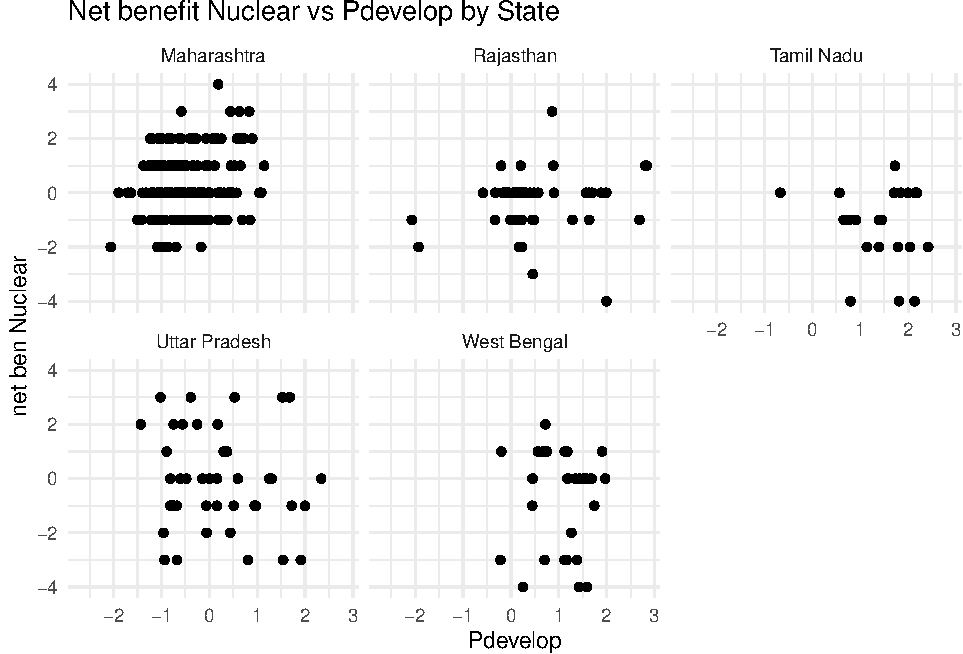
\includegraphics{FAoptions_files/figure-latex/unnamed-chunk-10-1.pdf}

\begin{verbatim}
## lavaan 0.6.15 ended normally after 17 iterations
## 
##   Estimator                                         ML
##   Optimization method                           NLMINB
##   Number of model parameters                        23
## 
##   Number of observations                           540
## 
## Model Test User Model:
##                                                       
##   Test statistic                               236.201
##   Degrees of freedom                                43
##   P-value (Chi-square)                           0.000
## 
## Model Test Baseline Model:
## 
##   Test statistic                              2291.291
##   Degrees of freedom                                55
##   P-value                                        0.000
## 
## User Model versus Baseline Model:
## 
##   Comparative Fit Index (CFI)                    0.914
##   Tucker-Lewis Index (TLI)                       0.889
## 
## Loglikelihood and Information Criteria:
## 
##   Loglikelihood user model (H0)              -8659.806
##   Loglikelihood unrestricted model (H1)      -8541.706
##                                                       
##   Akaike (AIC)                               17365.613
##   Bayesian (BIC)                             17464.319
##   Sample-size adjusted Bayesian (SABIC)      17391.309
## 
## Root Mean Square Error of Approximation:
## 
##   RMSEA                                          0.091
##   90 Percent confidence interval - lower         0.080
##   90 Percent confidence interval - upper         0.103
##   P-value H_0: RMSEA <= 0.050                    0.000
##   P-value H_0: RMSEA >= 0.080                    0.950
## 
## Standardized Root Mean Square Residual:
## 
##   SRMR                                           0.071
## 
## Parameter Estimates:
## 
##   Standard errors                             Standard
##   Information                                 Expected
##   Information saturated (h1) model          Structured
## 
## Latent Variables:
##                    Estimate  Std.Err  z-value  P(>|z|)   Std.lv  Std.all
##   Pdevelop =~                                                           
##     HEALTHSOLAR       0.970    0.049   19.888    0.000    0.970    0.779
##     BEAUTYSOLAR       0.820    0.052   15.860    0.000    0.820    0.654
##     DISPLACESOLAR     0.703    0.049   14.226    0.000    0.703    0.599
##     POLLUTESOLAR      1.096    0.050   22.088    0.000    1.096    0.843
##     INDUSTRYSMALL    -0.319    0.057   -5.571    0.000   -0.319   -0.255
##     OWNERREG         -0.315    0.051   -6.175    0.000   -0.315   -0.282
##     MECHANISATION    -0.452    0.052   -8.698    0.000   -0.452   -0.389
##   Ndevelop =~                                                           
##     DEVSOLAR          1.055    0.047   22.613    0.000    1.055    0.829
##     PRIDESOLAR        1.065    0.048   22.101    0.000    1.065    0.817
##     NPRIDESOLAR       1.009    0.047   21.327    0.000    1.009    0.797
##     PROSPERSOLAR      1.025    0.047   21.792    0.000    1.025    0.809
## 
## Covariances:
##                    Estimate  Std.Err  z-value  P(>|z|)   Std.lv  Std.all
##   Pdevelop ~~                                                           
##     Ndevelop         -0.262    0.047   -5.621    0.000   -0.262   -0.262
## 
## Variances:
##                    Estimate  Std.Err  z-value  P(>|z|)   Std.lv  Std.all
##    .HEALTHSOLAR       0.609    0.053   11.491    0.000    0.609    0.393
##    .BEAUTYSOLAR       0.902    0.064   14.185    0.000    0.902    0.573
##    .DISPLACESOLAR     0.882    0.060   14.768    0.000    0.882    0.641
##    .POLLUTESOLAR      0.490    0.055    8.917    0.000    0.490    0.290
##    .INDUSTRYSMALL     1.463    0.090   16.230    0.000    1.463    0.935
##    .OWNERREG          1.147    0.071   16.182    0.000    1.147    0.920
##    .MECHANISATION     1.143    0.072   15.912    0.000    1.143    0.848
##    .DEVSOLAR          0.505    0.043   11.626    0.000    0.505    0.312
##    .PRIDESOLAR        0.567    0.047   12.074    0.000    0.567    0.333
##    .NPRIDESOLAR       0.585    0.046   12.661    0.000    0.585    0.365
##    .PROSPERSOLAR      0.555    0.045   12.321    0.000    0.555    0.346
##     Pdevelop          1.000                               1.000    1.000
##     Ndevelop          1.000                               1.000    1.000
\end{verbatim}

\newpage

\hypertarget{solar-energy-cfa-on-combined-scale-2-factor-solution}{%
\subsection{Solar Energy : CFA on Combined Scale (2 Factor
Solution)}\label{solar-energy-cfa-on-combined-scale-2-factor-solution}}

Solar People Centered Development alpha = 0.75

Solar Nationalist Development alpha = 0.86

\begin{landscape}\begin{table}[!h]

\caption{\label{tab:unnamed-chunk-13}Confirmatory Factor Analysis(CFA) on Solar Energy}
\centering
\resizebox{\linewidth}{!}{
\begin{tabular}[t]{l>{\raggedright\arraybackslash}p{4cm}rrrrrrrr}
\toprule
Scale & Items & Loadings & Standard Error & zvalue & pvalue & ci.lower & ci.upper & std.lv & std.all\\
\midrule
\cellcolor{gray!6}{People Centered Development} & \cellcolor{gray!6}{Solar energy poses a great risk to the health of people living around it} & \cellcolor{gray!6}{0.970} & \cellcolor{gray!6}{0.049} & \cellcolor{gray!6}{19.888} & \cellcolor{gray!6}{0} & \cellcolor{gray!6}{0.8744108} & \cellcolor{gray!6}{1.0655965} & \cellcolor{gray!6}{0.9700037} & \cellcolor{gray!6}{0.7792714}\\
People Centered Development & Solar energy spoils the natural beauty of the landscape & 0.820 & 0.052 & 15.860 & 0 & 0.7190998 & 0.9218976 & 0.8204987 & 0.6537278\\
\cellcolor{gray!6}{People Centered Development} & \cellcolor{gray!6}{Solar energy is leading to displacement of people from their land} & \cellcolor{gray!6}{0.703} & \cellcolor{gray!6}{0.049} & \cellcolor{gray!6}{14.226} & \cellcolor{gray!6}{0} & \cellcolor{gray!6}{0.6057287} & \cellcolor{gray!6}{0.7993080} & \cellcolor{gray!6}{0.7025183} & \cellcolor{gray!6}{0.5989088}\\
People Centered Development & Solar energy increases pollution of air/water/land & 1.096 & 0.050 & 22.088 & 0 & 0.9990468 & 1.1936080 & 1.0963274 & 0.8428439\\
\cellcolor{gray!6}{People Centered Development} & \cellcolor{gray!6}{Large corporations are destroying the local industries in India and benefiting only a handful of people} & \cellcolor{gray!6}{-0.319} & \cellcolor{gray!6}{0.057} & \cellcolor{gray!6}{-5.571} & \cellcolor{gray!6}{0} & \cellcolor{gray!6}{-0.4318889} & \cellcolor{gray!6}{-0.2070914} & \cellcolor{gray!6}{-0.3194901} & \cellcolor{gray!6}{-0.2554075}\\
\addlinespace
People Centered Development & Regardless of ownership, the government should pass strong regulations and implement them & -0.315 & 0.051 & -6.175 & 0 & -0.4147132 & -0.2148716 & -0.3147924 & -0.2819769\\
\cellcolor{gray!6}{People Centered Development} & \cellcolor{gray!6}{Rapid mechanization of work is taking away jobs from workers in this country} & \cellcolor{gray!6}{-0.452} & \cellcolor{gray!6}{0.052} & \cellcolor{gray!6}{-8.698} & \cellcolor{gray!6}{0} & \cellcolor{gray!6}{-0.5538088} & \cellcolor{gray!6}{-0.3501230} & \cellcolor{gray!6}{-0.4519659} & \cellcolor{gray!6}{-0.3893190}\\
Nationalist Development & Solar energy pushes forward the country's development & 1.055 & 0.047 & 22.613 & 0 & 0.9638459 & 1.1467835 & 1.0553147 & 0.8294606\\
\cellcolor{gray!6}{Nationalist Development} & \cellcolor{gray!6}{I would be proud if my community used Solar energy} & \cellcolor{gray!6}{1.065} & \cellcolor{gray!6}{0.048} & \cellcolor{gray!6}{22.101} & \cellcolor{gray!6}{0} & \cellcolor{gray!6}{0.9708762} & \cellcolor{gray!6}{1.1598306} & \cellcolor{gray!6}{1.0653534} & \cellcolor{gray!6}{0.8166840}\\
Nationalist Development & Solar energy is a mark of pride for our nation & 1.009 & 0.047 & 21.327 & 0 & 0.9161682 & 1.1016049 & 1.0088866 & 0.7969797\\
\bottomrule
\end{tabular}}
\end{table}
\end{landscape}

\begin{verbatim}
## 
## Call:
## lm(formula = Risky_Solar ~ age + Uppercaste + Male + Hindu + 
##     Urban + State + KahanS + KahanH + Pdevelop + Ndevelop, data = sfascale_scores)
## 
## Residuals:
##     Min      1Q  Median      3Q     Max 
## -1.9138 -0.4677 -0.1288  0.2755  3.8143 
## 
## Coefficients:
##                     Estimate Std. Error t value Pr(>|t|)    
## (Intercept)         2.737482   0.143017  19.141  < 2e-16 ***
## age                -0.005030   0.035936  -0.140  0.88874    
## Uppercaste         -0.033151   0.082097  -0.404  0.68653    
## Male               -0.004959   0.090677  -0.055  0.95641    
## Hindu              -0.137916   0.095575  -1.443  0.14963    
## UrbanUrban         -0.066933   0.091671  -0.730  0.46564    
## StateRajasthan     -1.351258   0.143198  -9.436  < 2e-16 ***
## StateTamil Nadu    -1.314794   0.170603  -7.707 6.73e-14 ***
## StateUttar Pradesh -0.926163   0.158665  -5.837 9.42e-09 ***
## StateWest Bengal   -0.969840   0.185254  -5.235 2.41e-07 ***
## KahanS              0.031638   0.069903   0.453  0.65103    
## KahanH             -0.196447   0.067244  -2.921  0.00364 ** 
## Pdevelop            0.031323   0.061275   0.511  0.60943    
## Ndevelop            0.012994   0.053525   0.243  0.80828    
## ---
## Signif. codes:  0 '***' 0.001 '**' 0.01 '*' 0.05 '.' 0.1 ' ' 1
## 
## Residual standard error: 0.8389 on 513 degrees of freedom
##   (13 observations deleted due to missingness)
## Multiple R-squared:  0.4297, Adjusted R-squared:  0.4152 
## F-statistic: 29.73 on 13 and 513 DF,  p-value: < 2.2e-16
\end{verbatim}

\newpage

\hypertarget{coal-cfa-on-combined-scale-2-factor-solution-pdevelop-and-ndevelop}{%
\subsection{Coal : CFA on Combined Scale 2 Factor Solution (Pdevelop and
Ndevelop)}\label{coal-cfa-on-combined-scale-2-factor-solution-pdevelop-and-ndevelop}}

Coal People Centered Development Alpha = 0.78

Coal Nationalist Development Alpha = 0.6

\begin{landscape}\begin{table}[!h]

\caption{\label{tab:unnamed-chunk-18}Confirmatory Factor Analysis(CFA) on Coal}
\centering
\resizebox{\linewidth}{!}{
\begin{tabular}[t]{l>{\raggedright\arraybackslash}p{4cm}rrrrrrrr}
\toprule
Scale & Items & Loadings & Standard Error & zvalue & pvalue & ci.lower & ci.upper & std.lv & std.all\\
\midrule
\cellcolor{gray!6}{People Centered Development} & \cellcolor{gray!6}{Coal powered plants poses a great risk to the health of people living around it} & \cellcolor{gray!6}{0.722} & \cellcolor{gray!6}{0.050} & \cellcolor{gray!6}{14.378} & \cellcolor{gray!6}{0} & \cellcolor{gray!6}{0.6231797} & \cellcolor{gray!6}{0.8199012} & \cellcolor{gray!6}{0.7215405} & \cellcolor{gray!6}{0.6589018}\\
People Centered Development & Coal powered plants spoils the natural beauty of the landscape & 0.717 & 0.048 & 14.839 & 0 & 0.6227149 & 0.8122502 & 0.7174825 & 0.6758232\\
\cellcolor{gray!6}{People Centered Development} & \cellcolor{gray!6}{Coal powered plants is leading to displacement of people from their land} & \cellcolor{gray!6}{0.626} & \cellcolor{gray!6}{0.055} & \cellcolor{gray!6}{11.301} & \cellcolor{gray!6}{0} & \cellcolor{gray!6}{0.5172562} & \cellcolor{gray!6}{0.7343179} & \cellcolor{gray!6}{0.6257871} & \cellcolor{gray!6}{0.5394144}\\
People Centered Development & Coal powered plants increases pollution of air/water/land & 0.630 & 0.041 & 15.260 & 0 & 0.5488005 & 0.7105443 & 0.6296724 & 0.6910990\\
\cellcolor{gray!6}{People Centered Development} & \cellcolor{gray!6}{Large corporations are destroying the local industries in India and benefiting only a handful of people} & \cellcolor{gray!6}{0.601} & \cellcolor{gray!6}{0.057} & \cellcolor{gray!6}{10.462} & \cellcolor{gray!6}{0} & \cellcolor{gray!6}{0.4883282} & \cellcolor{gray!6}{0.7134684} & \cellcolor{gray!6}{0.6008983} & \cellcolor{gray!6}{0.5045829}\\
\addlinespace
People Centered Development & Regardless of ownership, the government should pass strong regulations and implement them & 0.488 & 0.055 & 8.904 & 0 & 0.3808612 & 0.5958528 & 0.4883570 & 0.4372022\\
\cellcolor{gray!6}{People Centered Development} & \cellcolor{gray!6}{Rapid mechanization of work is taking away jobs from workers in this country} & \cellcolor{gray!6}{0.658} & \cellcolor{gray!6}{0.056} & \cellcolor{gray!6}{11.805} & \cellcolor{gray!6}{0} & \cellcolor{gray!6}{0.5489483} & \cellcolor{gray!6}{0.7675273} & \cellcolor{gray!6}{0.6582378} & \cellcolor{gray!6}{0.5598383}\\
Nationalist Development & Coal powered plants pushes forward the country's development & 0.629 & 0.059 & 10.700 & 0 & 0.5137870 & 0.7442109 & 0.6289990 & 0.6259019\\
\cellcolor{gray!6}{Nationalist Development} & \cellcolor{gray!6}{Coal powered plants brings economic prosperity to the surrounding regions} & \cellcolor{gray!6}{0.596} & \cellcolor{gray!6}{0.058} & \cellcolor{gray!6}{10.338} & \cellcolor{gray!6}{0} & \cellcolor{gray!6}{0.4830019} & \cellcolor{gray!6}{0.7090010} & \cellcolor{gray!6}{0.5960014} & \cellcolor{gray!6}{0.5996861}\\
Nationalist Development & I would be proud if my community used Coal powered plants & 0.445 & 0.063 & 7.096 & 0 & 0.3220686 & 0.5678796 & 0.4449741 & 0.4027845\\
\bottomrule
\end{tabular}}
\end{table}
\end{landscape}

\newpage

\hypertarget{linear-models-perceived-risk-x-pdevelop-and-ndevelop}{%
\subsection{Linear Models: Perceived risk X Pdevelop and
Ndevelop}\label{linear-models-perceived-risk-x-pdevelop-and-ndevelop}}

\begingroup\setlength{\tabcolsep}{1pt}\renewcommand{\arraystretch}{0.7}

\% Table created by stargazer v.5.2.3 by Marek Hlavac, Social Policy
Institute. E-mail: marek.hlavac at gmail.com \% Date and time: Wed, Jan
10, 2024 - 10:07:32

\begin{table}[!htbp] \centering 
  \caption{Perceived Risk X Pdevelop and Ndevelope} 
  \label{} 
\begin{tabular}{@{\extracolsep{5pt}}lccc} 
\\[-1.8ex]\hline 
\hline \\[-1.8ex] 
 & \multicolumn{3}{c}{\textit{Dependent variable:}} \\ 
\cline{2-4} 
\\[-1.8ex] & Risky\_Nuclear & Risky\_Solar & Risky\_Coal \\ 
\\[-1.8ex] & (1) & (2) & (3)\\ 
\hline \\[-1.8ex] 
 age & 0.037 & $-$0.005 & 0.133$^{***}$ \\ 
  & (0.051) & (0.036) & (0.046) \\ 
  & & & \\ 
 Uppercaste & $-$0.035 & $-$0.033 & $-$0.060 \\ 
  & (0.106) & (0.082) & (0.090) \\ 
  & & & \\ 
 Male & $-$0.085 & $-$0.005 & 0.019 \\ 
  & (0.116) & (0.091) & (0.103) \\ 
  & & & \\ 
 Hindu & 0.024 & $-$0.138 & 0.155 \\ 
  & (0.117) & (0.096) & (0.106) \\ 
  & & & \\ 
 UrbanUrban & 0.023 & $-$0.067 & 0.051 \\ 
  & (0.111) & (0.092) & (0.102) \\ 
  & & & \\ 
 StateRajasthan & 0.190 & $-$1.351$^{***}$ & $-$0.349$^{**}$ \\ 
  & (0.181) & (0.143) & (0.142) \\ 
  & & & \\ 
 StateTamil Nadu & 1.293$^{***}$ & $-$1.315$^{***}$ & $-$1.387$^{***}$ \\ 
  & (0.239) & (0.171) & (0.226) \\ 
  & & & \\ 
 StateUttar Pradesh & $-$0.056 & $-$0.926$^{***}$ & $-$1.243$^{***}$ \\ 
  & (0.193) & (0.159) & (0.171) \\ 
  & & & \\ 
 StateWest Bengal & 0.972$^{***}$ & $-$0.970$^{***}$ & $-$0.124 \\ 
  & (0.226) & (0.185) & (0.198) \\ 
  & & & \\ 
 KahanS & 0.108 & 0.032 & 0.044 \\ 
  & (0.103) & (0.070) & (0.085) \\ 
  & & & \\ 
 KahanH & 0.003 & $-$0.196$^{***}$ & 0.148$^{*}$ \\ 
  & (0.095) & (0.067) & (0.086) \\ 
  & & & \\ 
 Pdevelop & 0.145$^{*}$ & 0.031 & 0.412$^{***}$ \\ 
  & (0.075) & (0.061) & (0.079) \\ 
  & & & \\ 
 Ndevelop & 0.236$^{***}$ & 0.013 & 0.031 \\ 
  & (0.061) & (0.054) & (0.067) \\ 
  & & & \\ 
 Constant & 3.028$^{***}$ & 2.737$^{***}$ & 3.069$^{***}$ \\ 
  & (0.172) & (0.143) & (0.157) \\ 
  & & & \\ 
\hline \\[-1.8ex] 
Observations & 405 & 527 & 457 \\ 
R$^{2}$ & 0.289 & 0.430 & 0.287 \\ 
Adjusted R$^{2}$ & 0.266 & 0.415 & 0.266 \\ 
Residual Std. Error & 0.925 (df = 391) & 0.839 (df = 513) & 0.877 (df = 443) \\ 
F Statistic & 12.248$^{***}$ (df = 13; 391) & 29.727$^{***}$ (df = 13; 513) & 13.728$^{***}$ (df = 13; 443) \\ 
\hline 
\hline \\[-1.8ex] 
\textit{Note:}  & \multicolumn{3}{r}{$^{*}$p$<$0.1; $^{**}$p$<$0.05; $^{***}$p$<$0.01} \\ 
\end{tabular} 
\end{table} 
\endgroup

\newpage

\hypertarget{linear-models-perceived-benefit-x-pdevelop-and-ndevelop}{%
\subsection{Linear Models: Perceived Benefit X Pdevelop and
Ndevelop}\label{linear-models-perceived-benefit-x-pdevelop-and-ndevelop}}

\begingroup\setlength{\tabcolsep}{1pt}

\renewcommand{\arraystretch}{0.7}

\% Table created by stargazer v.5.2.3 by Marek Hlavac, Social Policy
Institute. E-mail: marek.hlavac at gmail.com \% Date and time: Wed, Jan
10, 2024 - 10:07:33

\begin{table}[!htbp] \centering 
  \caption{Perceived Benefit X Pdevelop and Ndevelop} 
  \label{} 
\begin{tabular}{@{\extracolsep{5pt}}lccc} 
\\[-1.8ex]\hline 
\hline \\[-1.8ex] 
 & \multicolumn{3}{c}{\textit{Dependent variable:}} \\ 
\cline{2-4} 
\\[-1.8ex] & Ben\_Nuclear & Ben\_Solar & Ben\_Coal \\ 
\\[-1.8ex] & (1) & (2) & (3)\\ 
\hline \\[-1.8ex] 
 Uppercaste & $-$0.178$^{*}$ & $-$0.119 & $-$0.236$^{***}$ \\ 
  & (0.102) & (0.080) & (0.091) \\ 
  & & & \\ 
 Male & 0.036 & 0.0002 & 0.037 \\ 
  & (0.112) & (0.088) & (0.103) \\ 
  & & & \\ 
 Hindu & 0.329$^{***}$ & 0.169$^{*}$ & 0.039 \\ 
  & (0.113) & (0.093) & (0.107) \\ 
  & & & \\ 
 UrbanUrban & 0.093 & $-$0.081 & 0.169 \\ 
  & (0.107) & (0.089) & (0.103) \\ 
  & & & \\ 
 age & $-$0.073 & $-$0.023 & 0.029 \\ 
  & (0.050) & (0.034) & (0.046) \\ 
  & & & \\ 
 StateRajasthan & $-$0.573$^{***}$ & 0.495$^{***}$ & $-$0.327$^{**}$ \\ 
  & (0.175) & (0.147) & (0.142) \\ 
  & & & \\ 
 StateTamil Nadu & $-$0.406$^{*}$ & 0.564$^{***}$ & $-$0.316 \\ 
  & (0.235) & (0.177) & (0.238) \\ 
  & & & \\ 
 StateUttar Pradesh & $-$0.516$^{***}$ & 0.077 & $-$0.531$^{***}$ \\ 
  & (0.187) & (0.159) & (0.173) \\ 
  & & & \\ 
 StateWest Bengal & $-$0.095 & 0.943$^{***}$ & $-$0.169 \\ 
  & (0.222) & (0.184) & (0.198) \\ 
  & & & \\ 
 KahanS & $-$0.057 & 0.014 & $-$0.017 \\ 
  & (0.103) & (0.069) & (0.086) \\ 
  & & & \\ 
 KahanH & 0.231$^{**}$ & 0.140$^{**}$ & 0.141 \\ 
  & (0.093) & (0.070) & (0.087) \\ 
  & & & \\ 
 Pdevelop & 0.191$^{***}$ & 0.194$^{***}$ & 0.265$^{***}$ \\ 
  & (0.073) & (0.048) & (0.066) \\ 
  & & & \\ 
 Ndevelop & 0.292$^{***}$ & $-$0.018 & 0.213$^{***}$ \\ 
  & (0.060) & (0.068) & (0.049) \\ 
  & & & \\ 
 Constant & 3.287$^{***}$ & 3.426$^{***}$ & 3.205$^{***}$ \\ 
  & (0.166) & (0.139) & (0.157) \\ 
  & & & \\ 
\hline \\[-1.8ex] 
Observations & 407 & 535 & 455 \\ 
R$^{2}$ & 0.193 & 0.254 & 0.171 \\ 
Adjusted R$^{2}$ & 0.166 & 0.235 & 0.147 \\ 
Residual Std. Error & 0.898 (df = 393) & 0.815 (df = 521) & 0.880 (df = 441) \\ 
F Statistic & 7.210$^{***}$ (df = 13; 393) & 13.635$^{***}$ (df = 13; 521) & 7.020$^{***}$ (df = 13; 441) \\ 
\hline 
\hline \\[-1.8ex] 
\textit{Note:}  & \multicolumn{3}{r}{$^{*}$p$<$0.1; $^{**}$p$<$0.05; $^{***}$p$<$0.01} \\ 
\end{tabular} 
\end{table} 
\endgroup

\newpage

\hypertarget{linear-models-acceptance-risk---benefit-x-pdevelop-ndevelop}{%
\subsection{Linear Models: Acceptance (Risk - Benefit) X Pdevelop \&
Ndevelop}\label{linear-models-acceptance-risk---benefit-x-pdevelop-ndevelop}}

\begingroup\setlength{\tabcolsep}{1pt}

\renewcommand{\arraystretch}{0.7}

\% Table created by stargazer v.5.2.3 by Marek Hlavac, Social Policy
Institute. E-mail: marek.hlavac at gmail.com \% Date and time: Wed, Jan
10, 2024 - 10:07:33

\begin{table}[!htbp] \centering 
  \caption{Acceptance (Risk - Benefit) X Pdevelop and Ndevelop} 
  \label{} 
\begin{tabular}{@{\extracolsep{5pt}}lccc} 
\\[-1.8ex]\hline 
\hline \\[-1.8ex] 
 & \multicolumn{3}{c}{\textit{Dependent variable:}} \\ 
\cline{2-4} 
\\[-1.8ex] & Nuclear & Solar & Coal \\ 
\\[-1.8ex] & (1) & (2) & (3)\\ 
\hline \\[-1.8ex] 
 age & $-$0.108 & $-$0.016 & $-$0.148$^{**}$ \\ 
  & (0.069) & (0.053) & (0.062) \\ 
  & & & \\ 
 Uppercaste & $-$0.153 & $-$0.091 & $-$0.162 \\ 
  & (0.143) & (0.121) & (0.120) \\ 
  & & & \\ 
 Male & 0.146 & 0.015 & 0.013 \\ 
  & (0.157) & (0.133) & (0.137) \\ 
  & & & \\ 
 Hindu & 0.324$^{**}$ & 0.310$^{**}$ & $-$0.194 \\ 
  & (0.158) & (0.141) & (0.141) \\ 
  & & & \\ 
 UrbanUrban & 0.093 & 0.040 & 0.079 \\ 
  & (0.150) & (0.135) & (0.136) \\ 
  & & & \\ 
 StateRajasthan & $-$0.771$^{***}$ & 1.830$^{***}$ & 0.143 \\ 
  & (0.244) & (0.213) & (0.188) \\ 
  & & & \\ 
 StateTamil Nadu & $-$1.747$^{***}$ & 1.820$^{***}$ & 1.177$^{***}$ \\ 
  & (0.327) & (0.251) & (0.302) \\ 
  & & & \\ 
 StateUttar Pradesh & $-$0.462$^{*}$ & 0.990$^{***}$ & 0.791$^{***}$ \\ 
  & (0.261) & (0.235) & (0.228) \\ 
  & & & \\ 
 StateWest Bengal & $-$1.082$^{***}$ & 1.860$^{***}$ & $-$0.055 \\ 
  & (0.309) & (0.274) & (0.261) \\ 
  & & & \\ 
 KahanS & $-$0.193 & $-$0.044 & $-$0.042 \\ 
  & (0.139) & (0.103) & (0.113) \\ 
  & & & \\ 
 KahanH & 0.257$^{**}$ & 0.340$^{***}$ & 0.031 \\ 
  & (0.128) & (0.099) & (0.114) \\ 
  & & & \\ 
 Pdevelop & 0.023 & $-$0.039 & $-$0.374$^{***}$ \\ 
  & (0.103) & (0.090) & (0.106) \\ 
  & & & \\ 
 Ndevelop & 0.066 & 0.193$^{**}$ & 0.367$^{***}$ \\ 
  & (0.084) & (0.079) & (0.089) \\ 
  & & & \\ 
 Constant & 0.220 & 0.675$^{***}$ & 0.260 \\ 
  & (0.232) & (0.211) & (0.209) \\ 
  & & & \\ 
\hline \\[-1.8ex] 
Observations & 401 & 524 & 453 \\ 
R$^{2}$ & 0.164 & 0.471 & 0.099 \\ 
Adjusted R$^{2}$ & 0.136 & 0.458 & 0.072 \\ 
Residual Std. Error & 1.246 (df = 387) & 1.230 (df = 510) & 1.159 (df = 439) \\ 
F Statistic & 5.825$^{***}$ (df = 13; 387) & 34.992$^{***}$ (df = 13; 510) & 3.713$^{***}$ (df = 13; 439) \\ 
\hline 
\hline \\[-1.8ex] 
\textit{Note:}  & \multicolumn{3}{r}{$^{*}$p$<$0.1; $^{**}$p$<$0.05; $^{***}$p$<$0.01} \\ 
\end{tabular} 
\end{table} 
\endgroup

\newpage
\begin{landscape}

\hypertarget{fa-on-separate-scales-scale-1eco-political-values-of-the-perceiver}{%
\section{FA on Separate scales: Scale 1:Eco-political values of the
perceiver}\label{fa-on-separate-scales-scale-1eco-political-values-of-the-perceiver}}

\hypertarget{factor-solution-characteristics-of-the-perceiver}{%
\subsection{4 factor solution (Characteristics of the
perceiver)}\label{factor-solution-characteristics-of-the-perceiver}}

Cronbach's alpha values: Regulated Industrialisation = 0.59,
localisation = 0.52 , Free market = 0.57, Private Development = 0.58

\global\setlength{\Oldarrayrulewidth}{\arrayrulewidth}

\global\setlength{\Oldtabcolsep}{\tabcolsep}

\setlength{\tabcolsep}{0pt}

\renewcommand*{\arraystretch}{1.5}



\providecommand{\ascline}[3]{\noalign{\global\arrayrulewidth #1}\arrayrulecolor[HTML]{#2}\cline{#3}}

\begin{longtable}[c]{|p{1.50in}|p{3.50in}|p{0.50in}|p{0.50in}|p{0.50in}|p{0.50in}|p{0.75in}|p{0.75in}|p{0.75in}}

\caption{4\ factor\ solution\ same\ for\ all\ technologies}\\

\ascline{1.5pt}{666666}{1-9}

\multicolumn{1}{>{\raggedright}m{\dimexpr 1.5in+0\tabcolsep}}{\textcolor[HTML]{000000}{\fontsize{10}{10}\selectfont{code}}} & \multicolumn{1}{>{\raggedright}m{\dimexpr 3.5in+0\tabcolsep}}{\textcolor[HTML]{000000}{\fontsize{10}{10}\selectfont{Items}}} & \multicolumn{1}{>{\raggedright}m{\dimexpr 0.5in+0\tabcolsep}}{\textcolor[HTML]{000000}{\fontsize{10}{10}\selectfont{regulated\ industrialization}}} & \multicolumn{1}{>{\raggedright}m{\dimexpr 0.5in+0\tabcolsep}}{\textcolor[HTML]{000000}{\fontsize{10}{10}\selectfont{localisation}}} & \multicolumn{1}{>{\raggedright}m{\dimexpr 0.5in+0\tabcolsep}}{\textcolor[HTML]{000000}{\fontsize{10}{10}\selectfont{free\ market}}} & \multicolumn{1}{>{\raggedright}m{\dimexpr 0.5in+0\tabcolsep}}{\textcolor[HTML]{000000}{\fontsize{10}{10}\selectfont{private\ development}}} & \multicolumn{1}{>{\raggedleft}m{\dimexpr 0.75in+0\tabcolsep}}{\textcolor[HTML]{000000}{\fontsize{10}{10}\selectfont{Communality}}} & \multicolumn{1}{>{\raggedleft}m{\dimexpr 0.75in+0\tabcolsep}}{\textcolor[HTML]{000000}{\fontsize{10}{10}\selectfont{Uniqueness}}} & \multicolumn{1}{>{\raggedleft}m{\dimexpr 0.75in+0\tabcolsep}}{\textcolor[HTML]{000000}{\fontsize{10}{10}\selectfont{Complexity}}} \\

\ascline{1.5pt}{666666}{1-9}\endfirsthead \caption[]{4\ factor\ solution\ same\ for\ all\ technologies}\\

\ascline{1.5pt}{666666}{1-9}

\multicolumn{1}{>{\raggedright}m{\dimexpr 1.5in+0\tabcolsep}}{\textcolor[HTML]{000000}{\fontsize{10}{10}\selectfont{code}}} & \multicolumn{1}{>{\raggedright}m{\dimexpr 3.5in+0\tabcolsep}}{\textcolor[HTML]{000000}{\fontsize{10}{10}\selectfont{Items}}} & \multicolumn{1}{>{\raggedright}m{\dimexpr 0.5in+0\tabcolsep}}{\textcolor[HTML]{000000}{\fontsize{10}{10}\selectfont{regulated\ industrialization}}} & \multicolumn{1}{>{\raggedright}m{\dimexpr 0.5in+0\tabcolsep}}{\textcolor[HTML]{000000}{\fontsize{10}{10}\selectfont{localisation}}} & \multicolumn{1}{>{\raggedright}m{\dimexpr 0.5in+0\tabcolsep}}{\textcolor[HTML]{000000}{\fontsize{10}{10}\selectfont{free\ market}}} & \multicolumn{1}{>{\raggedright}m{\dimexpr 0.5in+0\tabcolsep}}{\textcolor[HTML]{000000}{\fontsize{10}{10}\selectfont{private\ development}}} & \multicolumn{1}{>{\raggedleft}m{\dimexpr 0.75in+0\tabcolsep}}{\textcolor[HTML]{000000}{\fontsize{10}{10}\selectfont{Communality}}} & \multicolumn{1}{>{\raggedleft}m{\dimexpr 0.75in+0\tabcolsep}}{\textcolor[HTML]{000000}{\fontsize{10}{10}\selectfont{Uniqueness}}} & \multicolumn{1}{>{\raggedleft}m{\dimexpr 0.75in+0\tabcolsep}}{\textcolor[HTML]{000000}{\fontsize{10}{10}\selectfont{Complexity}}} \\

\ascline{1.5pt}{666666}{1-9}\endhead



\multicolumn{1}{>{\raggedright}m{\dimexpr 1.5in+0\tabcolsep}}{\textcolor[HTML]{000000}{\fontsize{10}{10}\selectfont{Pro\ Regulations}}} & \multicolumn{1}{>{\raggedright}m{\dimexpr 3.5in+0\tabcolsep}}{\textcolor[HTML]{000000}{\fontsize{10}{10}\selectfont{Regardless\ of\ ownership,\ the\ government\ should\ pass\ strong\ regulations\ and\ implement\ them}}} & \multicolumn{1}{>{\raggedright}m{\dimexpr 0.5in+0\tabcolsep}}{\textcolor[HTML]{000000}{\fontsize{10}{10}\selectfont{0.54}}} & \multicolumn{1}{>{\raggedright}m{\dimexpr 0.5in+0\tabcolsep}}{\textcolor[HTML]{000000}{\fontsize{10}{10}\selectfont{}}} & \multicolumn{1}{>{\raggedright}m{\dimexpr 0.5in+0\tabcolsep}}{\textcolor[HTML]{000000}{\fontsize{10}{10}\selectfont{}}} & \multicolumn{1}{>{\raggedright}m{\dimexpr 0.5in+0\tabcolsep}}{\textcolor[HTML]{000000}{\fontsize{10}{10}\selectfont{}}} & \multicolumn{1}{>{\raggedleft}m{\dimexpr 0.75in+0\tabcolsep}}{\textcolor[HTML]{000000}{\fontsize{10}{10}\selectfont{0.366}}} & \multicolumn{1}{>{\raggedleft}m{\dimexpr 0.75in+0\tabcolsep}}{\textcolor[HTML]{000000}{\fontsize{10}{10}\selectfont{0.634}}} & \multicolumn{1}{>{\raggedleft}m{\dimexpr 0.75in+0\tabcolsep}}{\textcolor[HTML]{000000}{\fontsize{10}{10}\selectfont{1.520}}} \\





\multicolumn{1}{>{\raggedright}m{\dimexpr 1.5in+0\tabcolsep}}{\textcolor[HTML]{000000}{\fontsize{10}{10}\selectfont{Anti\ Mechanisation\ of\ work}}} & \multicolumn{1}{>{\raggedright}m{\dimexpr 3.5in+0\tabcolsep}}{\textcolor[HTML]{000000}{\fontsize{10}{10}\selectfont{Rapid\ mechanization\ of\ work\ is\ taking\ away\ jobs\ from\ workers\ in\ this\ country}}} & \multicolumn{1}{>{\raggedright}m{\dimexpr 0.5in+0\tabcolsep}}{\textcolor[HTML]{000000}{\fontsize{10}{10}\selectfont{0.506}}} & \multicolumn{1}{>{\raggedright}m{\dimexpr 0.5in+0\tabcolsep}}{\textcolor[HTML]{000000}{\fontsize{10}{10}\selectfont{}}} & \multicolumn{1}{>{\raggedright}m{\dimexpr 0.5in+0\tabcolsep}}{\textcolor[HTML]{000000}{\fontsize{10}{10}\selectfont{}}} & \multicolumn{1}{>{\raggedright}m{\dimexpr 0.5in+0\tabcolsep}}{\textcolor[HTML]{000000}{\fontsize{10}{10}\selectfont{}}} & \multicolumn{1}{>{\raggedleft}m{\dimexpr 0.75in+0\tabcolsep}}{\textcolor[HTML]{000000}{\fontsize{10}{10}\selectfont{0.330}}} & \multicolumn{1}{>{\raggedleft}m{\dimexpr 0.75in+0\tabcolsep}}{\textcolor[HTML]{000000}{\fontsize{10}{10}\selectfont{0.670}}} & \multicolumn{1}{>{\raggedleft}m{\dimexpr 0.75in+0\tabcolsep}}{\textcolor[HTML]{000000}{\fontsize{10}{10}\selectfont{1.585}}} \\





\multicolumn{1}{>{\raggedright}m{\dimexpr 1.5in+0\tabcolsep}}{\textcolor[HTML]{000000}{\fontsize{10}{10}\selectfont{Limits\ on\ Wealth}}} & \multicolumn{1}{>{\raggedright}m{\dimexpr 3.5in+0\tabcolsep}}{\textcolor[HTML]{000000}{\fontsize{10}{10}\selectfont{A\ limit\ should\ be\ put\ to\ how\ much\ wealth\ a\ person\ can\ amass}}} & \multicolumn{1}{>{\raggedright}m{\dimexpr 0.5in+0\tabcolsep}}{\textcolor[HTML]{000000}{\fontsize{10}{10}\selectfont{0.483}}} & \multicolumn{1}{>{\raggedright}m{\dimexpr 0.5in+0\tabcolsep}}{\textcolor[HTML]{000000}{\fontsize{10}{10}\selectfont{}}} & \multicolumn{1}{>{\raggedright}m{\dimexpr 0.5in+0\tabcolsep}}{\textcolor[HTML]{000000}{\fontsize{10}{10}\selectfont{}}} & \multicolumn{1}{>{\raggedright}m{\dimexpr 0.5in+0\tabcolsep}}{\textcolor[HTML]{000000}{\fontsize{10}{10}\selectfont{}}} & \multicolumn{1}{>{\raggedleft}m{\dimexpr 0.75in+0\tabcolsep}}{\textcolor[HTML]{000000}{\fontsize{10}{10}\selectfont{0.304}}} & \multicolumn{1}{>{\raggedleft}m{\dimexpr 0.75in+0\tabcolsep}}{\textcolor[HTML]{000000}{\fontsize{10}{10}\selectfont{0.696}}} & \multicolumn{1}{>{\raggedleft}m{\dimexpr 0.75in+0\tabcolsep}}{\textcolor[HTML]{000000}{\fontsize{10}{10}\selectfont{1.638}}} \\





\multicolumn{1}{>{\raggedright}m{\dimexpr 1.5in+0\tabcolsep}}{\textcolor[HTML]{000000}{\fontsize{10}{10}\selectfont{Anti\ Large\ Industries}}} & \multicolumn{1}{>{\raggedright}m{\dimexpr 3.5in+0\tabcolsep}}{\textcolor[HTML]{000000}{\fontsize{10}{10}\selectfont{Large\ corporations\ are\ destroying\ the\ local\ industries\ in\ India\ and\ benefiting\ only\ a\ handful\ of\ people}}} & \multicolumn{1}{>{\raggedright}m{\dimexpr 0.5in+0\tabcolsep}}{\textcolor[HTML]{000000}{\fontsize{10}{10}\selectfont{}}} & \multicolumn{1}{>{\raggedright}m{\dimexpr 0.5in+0\tabcolsep}}{\textcolor[HTML]{000000}{\fontsize{10}{10}\selectfont{0.534}}} & \multicolumn{1}{>{\raggedright}m{\dimexpr 0.5in+0\tabcolsep}}{\textcolor[HTML]{000000}{\fontsize{10}{10}\selectfont{}}} & \multicolumn{1}{>{\raggedright}m{\dimexpr 0.5in+0\tabcolsep}}{\textcolor[HTML]{000000}{\fontsize{10}{10}\selectfont{}}} & \multicolumn{1}{>{\raggedleft}m{\dimexpr 0.75in+0\tabcolsep}}{\textcolor[HTML]{000000}{\fontsize{10}{10}\selectfont{0.409}}} & \multicolumn{1}{>{\raggedleft}m{\dimexpr 0.75in+0\tabcolsep}}{\textcolor[HTML]{000000}{\fontsize{10}{10}\selectfont{0.591}}} & \multicolumn{1}{>{\raggedleft}m{\dimexpr 0.75in+0\tabcolsep}}{\textcolor[HTML]{000000}{\fontsize{10}{10}\selectfont{1.780}}} \\





\multicolumn{1}{>{\raggedright}m{\dimexpr 1.5in+0\tabcolsep}}{\textcolor[HTML]{000000}{\fontsize{10}{10}\selectfont{Pro\ Localeconomy}}} & \multicolumn{1}{>{\raggedright}m{\dimexpr 3.5in+0\tabcolsep}}{\textcolor[HTML]{000000}{\fontsize{10}{10}\selectfont{India\ would\ be\ better\ off\ if\ foreign\ companies\ didn't\ come\ to\ here}}} & \multicolumn{1}{>{\raggedright}m{\dimexpr 0.5in+0\tabcolsep}}{\textcolor[HTML]{000000}{\fontsize{10}{10}\selectfont{}}} & \multicolumn{1}{>{\raggedright}m{\dimexpr 0.5in+0\tabcolsep}}{\textcolor[HTML]{000000}{\fontsize{10}{10}\selectfont{0.524}}} & \multicolumn{1}{>{\raggedright}m{\dimexpr 0.5in+0\tabcolsep}}{\textcolor[HTML]{000000}{\fontsize{10}{10}\selectfont{}}} & \multicolumn{1}{>{\raggedright}m{\dimexpr 0.5in+0\tabcolsep}}{\textcolor[HTML]{000000}{\fontsize{10}{10}\selectfont{}}} & \multicolumn{1}{>{\raggedleft}m{\dimexpr 0.75in+0\tabcolsep}}{\textcolor[HTML]{000000}{\fontsize{10}{10}\selectfont{0.287}}} & \multicolumn{1}{>{\raggedleft}m{\dimexpr 0.75in+0\tabcolsep}}{\textcolor[HTML]{000000}{\fontsize{10}{10}\selectfont{0.713}}} & \multicolumn{1}{>{\raggedleft}m{\dimexpr 0.75in+0\tabcolsep}}{\textcolor[HTML]{000000}{\fontsize{10}{10}\selectfont{1.090}}} \\





\multicolumn{1}{>{\raggedright}m{\dimexpr 1.5in+0\tabcolsep}}{\textcolor[HTML]{000000}{\fontsize{10}{10}\selectfont{Pro\ Decentralisation}}} & \multicolumn{1}{>{\raggedright}m{\dimexpr 3.5in+0\tabcolsep}}{\textcolor[HTML]{000000}{\fontsize{10}{10}\selectfont{Local\ politicians\ shouldn't\ have\ to\ ask\ permission\ from\ the\ central\ government\ to\ implement\ policies}}} & \multicolumn{1}{>{\raggedright}m{\dimexpr 0.5in+0\tabcolsep}}{\textcolor[HTML]{000000}{\fontsize{10}{10}\selectfont{}}} & \multicolumn{1}{>{\raggedright}m{\dimexpr 0.5in+0\tabcolsep}}{\textcolor[HTML]{000000}{\fontsize{10}{10}\selectfont{}}} & \multicolumn{1}{>{\raggedright}m{\dimexpr 0.5in+0\tabcolsep}}{\textcolor[HTML]{000000}{\fontsize{10}{10}\selectfont{}}} & \multicolumn{1}{>{\raggedright}m{\dimexpr 0.5in+0\tabcolsep}}{\textcolor[HTML]{000000}{\fontsize{10}{10}\selectfont{}}} & \multicolumn{1}{>{\raggedleft}m{\dimexpr 0.75in+0\tabcolsep}}{\textcolor[HTML]{000000}{\fontsize{10}{10}\selectfont{0.134}}} & \multicolumn{1}{>{\raggedleft}m{\dimexpr 0.75in+0\tabcolsep}}{\textcolor[HTML]{000000}{\fontsize{10}{10}\selectfont{0.866}}} & \multicolumn{1}{>{\raggedleft}m{\dimexpr 0.75in+0\tabcolsep}}{\textcolor[HTML]{000000}{\fontsize{10}{10}\selectfont{2.021}}} \\





\multicolumn{1}{>{\raggedright}m{\dimexpr 1.5in+0\tabcolsep}}{\textcolor[HTML]{000000}{\fontsize{10}{10}\selectfont{Pro\ Centralisation}}} & \multicolumn{1}{>{\raggedright}m{\dimexpr 3.5in+0\tabcolsep}}{\textcolor[HTML]{000000}{\fontsize{10}{10}\selectfont{Laws\ and\ policies\ would\ be\ implemented\ more\ smoothly\ if\ more\ power\ lay\ with\ the\ central\ government}}} & \multicolumn{1}{>{\raggedright}m{\dimexpr 0.5in+0\tabcolsep}}{\textcolor[HTML]{000000}{\fontsize{10}{10}\selectfont{}}} & \multicolumn{1}{>{\raggedright}m{\dimexpr 0.5in+0\tabcolsep}}{\textcolor[HTML]{000000}{\fontsize{10}{10}\selectfont{}}} & \multicolumn{1}{>{\raggedright}m{\dimexpr 0.5in+0\tabcolsep}}{\textcolor[HTML]{000000}{\fontsize{10}{10}\selectfont{0.488}}} & \multicolumn{1}{>{\raggedright}m{\dimexpr 0.5in+0\tabcolsep}}{\textcolor[HTML]{000000}{\fontsize{10}{10}\selectfont{}}} & \multicolumn{1}{>{\raggedleft}m{\dimexpr 0.75in+0\tabcolsep}}{\textcolor[HTML]{000000}{\fontsize{10}{10}\selectfont{0.280}}} & \multicolumn{1}{>{\raggedleft}m{\dimexpr 0.75in+0\tabcolsep}}{\textcolor[HTML]{000000}{\fontsize{10}{10}\selectfont{0.720}}} & \multicolumn{1}{>{\raggedleft}m{\dimexpr 0.75in+0\tabcolsep}}{\textcolor[HTML]{000000}{\fontsize{10}{10}\selectfont{1.360}}} \\





\multicolumn{1}{>{\raggedright}m{\dimexpr 1.5in+0\tabcolsep}}{\textcolor[HTML]{000000}{\fontsize{10}{10}\selectfont{Pro\ Globaleconomy}}} & \multicolumn{1}{>{\raggedright}m{\dimexpr 3.5in+0\tabcolsep}}{\textcolor[HTML]{000000}{\fontsize{10}{10}\selectfont{Foreign\ companies\ have\ led\ to\ a\ range\ of\ benefits\ for\ the\ Indian\ people\ and\ society}}} & \multicolumn{1}{>{\raggedright}m{\dimexpr 0.5in+0\tabcolsep}}{\textcolor[HTML]{000000}{\fontsize{10}{10}\selectfont{}}} & \multicolumn{1}{>{\raggedright}m{\dimexpr 0.5in+0\tabcolsep}}{\textcolor[HTML]{000000}{\fontsize{10}{10}\selectfont{}}} & \multicolumn{1}{>{\raggedright}m{\dimexpr 0.5in+0\tabcolsep}}{\textcolor[HTML]{000000}{\fontsize{10}{10}\selectfont{0.478}}} & \multicolumn{1}{>{\raggedright}m{\dimexpr 0.5in+0\tabcolsep}}{\textcolor[HTML]{000000}{\fontsize{10}{10}\selectfont{}}} & \multicolumn{1}{>{\raggedleft}m{\dimexpr 0.75in+0\tabcolsep}}{\textcolor[HTML]{000000}{\fontsize{10}{10}\selectfont{0.298}}} & \multicolumn{1}{>{\raggedleft}m{\dimexpr 0.75in+0\tabcolsep}}{\textcolor[HTML]{000000}{\fontsize{10}{10}\selectfont{0.702}}} & \multicolumn{1}{>{\raggedleft}m{\dimexpr 0.75in+0\tabcolsep}}{\textcolor[HTML]{000000}{\fontsize{10}{10}\selectfont{1.598}}} \\





\multicolumn{1}{>{\raggedright}m{\dimexpr 1.5in+0\tabcolsep}}{\textcolor[HTML]{000000}{\fontsize{10}{10}\selectfont{Anti\ Regulations}}} & \multicolumn{1}{>{\raggedright}m{\dimexpr 3.5in+0\tabcolsep}}{\textcolor[HTML]{000000}{\fontsize{10}{10}\selectfont{There\ is\ too\ much\ red-tape\ and\ the\ government\ should\ not\ interfere\ with\ businesses\ and\ industries}}} & \multicolumn{1}{>{\raggedright}m{\dimexpr 0.5in+0\tabcolsep}}{\textcolor[HTML]{000000}{\fontsize{10}{10}\selectfont{}}} & \multicolumn{1}{>{\raggedright}m{\dimexpr 0.5in+0\tabcolsep}}{\textcolor[HTML]{000000}{\fontsize{10}{10}\selectfont{}}} & \multicolumn{1}{>{\raggedright}m{\dimexpr 0.5in+0\tabcolsep}}{\textcolor[HTML]{000000}{\fontsize{10}{10}\selectfont{0.473}}} & \multicolumn{1}{>{\raggedright}m{\dimexpr 0.5in+0\tabcolsep}}{\textcolor[HTML]{000000}{\fontsize{10}{10}\selectfont{}}} & \multicolumn{1}{>{\raggedleft}m{\dimexpr 0.75in+0\tabcolsep}}{\textcolor[HTML]{000000}{\fontsize{10}{10}\selectfont{0.399}}} & \multicolumn{1}{>{\raggedleft}m{\dimexpr 0.75in+0\tabcolsep}}{\textcolor[HTML]{000000}{\fontsize{10}{10}\selectfont{0.601}}} & \multicolumn{1}{>{\raggedleft}m{\dimexpr 0.75in+0\tabcolsep}}{\textcolor[HTML]{000000}{\fontsize{10}{10}\selectfont{2.220}}} \\





\multicolumn{1}{>{\raggedright}m{\dimexpr 1.5in+0\tabcolsep}}{\textcolor[HTML]{000000}{\fontsize{10}{10}\selectfont{Pro\ Large\ Industries}}} & \multicolumn{1}{>{\raggedright}m{\dimexpr 3.5in+0\tabcolsep}}{\textcolor[HTML]{000000}{\fontsize{10}{10}\selectfont{Large\ scale\ industries\ are\ required\ for\ the\ development\ of\ the\ country\ that\ will\ benefit\ everyone}}} & \multicolumn{1}{>{\raggedright}m{\dimexpr 0.5in+0\tabcolsep}}{\textcolor[HTML]{000000}{\fontsize{10}{10}\selectfont{}}} & \multicolumn{1}{>{\raggedright}m{\dimexpr 0.5in+0\tabcolsep}}{\textcolor[HTML]{000000}{\fontsize{10}{10}\selectfont{}}} & \multicolumn{1}{>{\raggedright}m{\dimexpr 0.5in+0\tabcolsep}}{\textcolor[HTML]{000000}{\fontsize{10}{10}\selectfont{0.432}}} & \multicolumn{1}{>{\raggedright}m{\dimexpr 0.5in+0\tabcolsep}}{\textcolor[HTML]{000000}{\fontsize{10}{10}\selectfont{}}} & \multicolumn{1}{>{\raggedleft}m{\dimexpr 0.75in+0\tabcolsep}}{\textcolor[HTML]{000000}{\fontsize{10}{10}\selectfont{0.302}}} & \multicolumn{1}{>{\raggedleft}m{\dimexpr 0.75in+0\tabcolsep}}{\textcolor[HTML]{000000}{\fontsize{10}{10}\selectfont{0.698}}} & \multicolumn{1}{>{\raggedleft}m{\dimexpr 0.75in+0\tabcolsep}}{\textcolor[HTML]{000000}{\fontsize{10}{10}\selectfont{1.902}}} \\





\multicolumn{1}{>{\raggedright}m{\dimexpr 1.5in+0\tabcolsep}}{\textcolor[HTML]{000000}{\fontsize{10}{10}\selectfont{Development\ over\ Environment}}} & \multicolumn{1}{>{\raggedright}m{\dimexpr 3.5in+0\tabcolsep}}{\textcolor[HTML]{000000}{\fontsize{10}{10}\selectfont{Economic\ growth\ and\ creating\ jobs\ should\ be\ prioritized\ over\ environmental\ protection}}} & \multicolumn{1}{>{\raggedright}m{\dimexpr 0.5in+0\tabcolsep}}{\textcolor[HTML]{000000}{\fontsize{10}{10}\selectfont{}}} & \multicolumn{1}{>{\raggedright}m{\dimexpr 0.5in+0\tabcolsep}}{\textcolor[HTML]{000000}{\fontsize{10}{10}\selectfont{}}} & \multicolumn{1}{>{\raggedright}m{\dimexpr 0.5in+0\tabcolsep}}{\textcolor[HTML]{000000}{\fontsize{10}{10}\selectfont{}}} & \multicolumn{1}{>{\raggedright}m{\dimexpr 0.5in+0\tabcolsep}}{\textcolor[HTML]{000000}{\fontsize{10}{10}\selectfont{0.536}}} & \multicolumn{1}{>{\raggedleft}m{\dimexpr 0.75in+0\tabcolsep}}{\textcolor[HTML]{000000}{\fontsize{10}{10}\selectfont{0.290}}} & \multicolumn{1}{>{\raggedleft}m{\dimexpr 0.75in+0\tabcolsep}}{\textcolor[HTML]{000000}{\fontsize{10}{10}\selectfont{0.710}}} & \multicolumn{1}{>{\raggedleft}m{\dimexpr 0.75in+0\tabcolsep}}{\textcolor[HTML]{000000}{\fontsize{10}{10}\selectfont{1.014}}} \\





\multicolumn{1}{>{\raggedright}m{\dimexpr 1.5in+0\tabcolsep}}{\textcolor[HTML]{000000}{\fontsize{10}{10}\selectfont{Pro\ Private\ ownership}}} & \multicolumn{1}{>{\raggedright}m{\dimexpr 3.5in+0\tabcolsep}}{\textcolor[HTML]{000000}{\fontsize{10}{10}\selectfont{All\ businesses\ and\ industries\ should\ be\ owned\ privately}}} & \multicolumn{1}{>{\raggedright}m{\dimexpr 0.5in+0\tabcolsep}}{\textcolor[HTML]{000000}{\fontsize{10}{10}\selectfont{}}} & \multicolumn{1}{>{\raggedright}m{\dimexpr 0.5in+0\tabcolsep}}{\textcolor[HTML]{000000}{\fontsize{10}{10}\selectfont{}}} & \multicolumn{1}{>{\raggedright}m{\dimexpr 0.5in+0\tabcolsep}}{\textcolor[HTML]{000000}{\fontsize{10}{10}\selectfont{}}} & \multicolumn{1}{>{\raggedright}m{\dimexpr 0.5in+0\tabcolsep}}{\textcolor[HTML]{000000}{\fontsize{10}{10}\selectfont{0.508}}} & \multicolumn{1}{>{\raggedleft}m{\dimexpr 0.75in+0\tabcolsep}}{\textcolor[HTML]{000000}{\fontsize{10}{10}\selectfont{0.274}}} & \multicolumn{1}{>{\raggedleft}m{\dimexpr 0.75in+0\tabcolsep}}{\textcolor[HTML]{000000}{\fontsize{10}{10}\selectfont{0.726}}} & \multicolumn{1}{>{\raggedleft}m{\dimexpr 0.75in+0\tabcolsep}}{\textcolor[HTML]{000000}{\fontsize{10}{10}\selectfont{1.121}}} \\





\multicolumn{1}{>{\raggedright}m{\dimexpr 1.5in+0\tabcolsep}}{\textcolor[HTML]{000000}{\fontsize{10}{10}\selectfont{Environment\ over\ Development}}} & \multicolumn{1}{>{\raggedright}m{\dimexpr 3.5in+0\tabcolsep}}{\textcolor[HTML]{000000}{\fontsize{10}{10}\selectfont{Polluting\ industries\ that\ spoil\ the\ environment\ should\ be\ shut\ down\ even\ if\ it\ costs\ people\ their\ jobs}}} & \multicolumn{1}{>{\raggedright}m{\dimexpr 0.5in+0\tabcolsep}}{\textcolor[HTML]{000000}{\fontsize{10}{10}\selectfont{}}} & \multicolumn{1}{>{\raggedright}m{\dimexpr 0.5in+0\tabcolsep}}{\textcolor[HTML]{000000}{\fontsize{10}{10}\selectfont{}}} & \multicolumn{1}{>{\raggedright}m{\dimexpr 0.5in+0\tabcolsep}}{\textcolor[HTML]{000000}{\fontsize{10}{10}\selectfont{}}} & \multicolumn{1}{>{\raggedright}m{\dimexpr 0.5in+0\tabcolsep}}{\textcolor[HTML]{000000}{\fontsize{10}{10}\selectfont{-0.464}}} & \multicolumn{1}{>{\raggedleft}m{\dimexpr 0.75in+0\tabcolsep}}{\textcolor[HTML]{000000}{\fontsize{10}{10}\selectfont{0.428}}} & \multicolumn{1}{>{\raggedleft}m{\dimexpr 0.75in+0\tabcolsep}}{\textcolor[HTML]{000000}{\fontsize{10}{10}\selectfont{0.572}}} & \multicolumn{1}{>{\raggedleft}m{\dimexpr 0.75in+0\tabcolsep}}{\textcolor[HTML]{000000}{\fontsize{10}{10}\selectfont{2.548}}} \\





\multicolumn{1}{>{\raggedright}m{\dimexpr 1.5in+0\tabcolsep}}{\textcolor[HTML]{000000}{\fontsize{10}{10}\selectfont{Pro\ Public\ ownership}}} & \multicolumn{1}{>{\raggedright}m{\dimexpr 3.5in+0\tabcolsep}}{\textcolor[HTML]{000000}{\fontsize{10}{10}\selectfont{The\ government\ should\ own\ most\ large\ businesses\ and\ industries}}} & \multicolumn{1}{>{\raggedright}m{\dimexpr 0.5in+0\tabcolsep}}{\textcolor[HTML]{000000}{\fontsize{10}{10}\selectfont{}}} & \multicolumn{1}{>{\raggedright}m{\dimexpr 0.5in+0\tabcolsep}}{\textcolor[HTML]{000000}{\fontsize{10}{10}\selectfont{}}} & \multicolumn{1}{>{\raggedright}m{\dimexpr 0.5in+0\tabcolsep}}{\textcolor[HTML]{000000}{\fontsize{10}{10}\selectfont{}}} & \multicolumn{1}{>{\raggedright}m{\dimexpr 0.5in+0\tabcolsep}}{\textcolor[HTML]{000000}{\fontsize{10}{10}\selectfont{-0.43}}} & \multicolumn{1}{>{\raggedleft}m{\dimexpr 0.75in+0\tabcolsep}}{\textcolor[HTML]{000000}{\fontsize{10}{10}\selectfont{0.433}}} & \multicolumn{1}{>{\raggedleft}m{\dimexpr 0.75in+0\tabcolsep}}{\textcolor[HTML]{000000}{\fontsize{10}{10}\selectfont{0.567}}} & \multicolumn{1}{>{\raggedleft}m{\dimexpr 0.75in+0\tabcolsep}}{\textcolor[HTML]{000000}{\fontsize{10}{10}\selectfont{3.201}}} \\

\ascline{1.5pt}{666666}{1-9}



\end{longtable}



\arrayrulecolor[HTML]{000000}

\global\setlength{\arrayrulewidth}{\Oldarrayrulewidth}

\global\setlength{\tabcolsep}{\Oldtabcolsep}

\renewcommand*{\arraystretch}{1}

\end{landscape}

\global\setlength{\Oldarrayrulewidth}{\arrayrulewidth}

\global\setlength{\Oldtabcolsep}{\tabcolsep}

\setlength{\tabcolsep}{0pt}

\renewcommand*{\arraystretch}{1.5}



\providecommand{\ascline}[3]{\noalign{\global\arrayrulewidth #1}\arrayrulecolor[HTML]{#2}\cline{#3}}

\begin{longtable}[c]{ccccc}

\caption{Eigenvalues\ and\ Variance\ Explained\ for\ Rotated\ Factor\ Solution}\\

\ascline{1.5pt}{666666}{1-5}

\multicolumn{1}{>{}l}{\textcolor[HTML]{000000}{\fontsize{10}{10}\selectfont{Property}}} & \multicolumn{1}{>{}r}{\textcolor[HTML]{000000}{\fontsize{10}{10}\selectfont{MR1}}} & \multicolumn{1}{>{}r}{\textcolor[HTML]{000000}{\fontsize{10}{10}\selectfont{MR3}}} & \multicolumn{1}{>{}r}{\textcolor[HTML]{000000}{\fontsize{10}{10}\selectfont{MR4}}} & \multicolumn{1}{>{}r}{\textcolor[HTML]{000000}{\fontsize{10}{10}\selectfont{MR2}}} \\

\ascline{1.5pt}{666666}{1-5}\endfirsthead \caption[]{Eigenvalues\ and\ Variance\ Explained\ for\ Rotated\ Factor\ Solution}\\

\ascline{1.5pt}{666666}{1-5}

\multicolumn{1}{>{}l}{\textcolor[HTML]{000000}{\fontsize{10}{10}\selectfont{Property}}} & \multicolumn{1}{>{}r}{\textcolor[HTML]{000000}{\fontsize{10}{10}\selectfont{MR1}}} & \multicolumn{1}{>{}r}{\textcolor[HTML]{000000}{\fontsize{10}{10}\selectfont{MR3}}} & \multicolumn{1}{>{}r}{\textcolor[HTML]{000000}{\fontsize{10}{10}\selectfont{MR4}}} & \multicolumn{1}{>{}r}{\textcolor[HTML]{000000}{\fontsize{10}{10}\selectfont{MR2}}} \\

\ascline{1.5pt}{666666}{1-5}\endhead



\multicolumn{1}{>{}l}{\textcolor[HTML]{000000}{\fontsize{10}{10}\selectfont{SS\ loadings}}} & \multicolumn{1}{>{}r}{\textcolor[HTML]{000000}{\fontsize{10}{10}\selectfont{1.215}}} & \multicolumn{1}{>{}r}{\textcolor[HTML]{000000}{\fontsize{10}{10}\selectfont{1.191}}} & \multicolumn{1}{>{}r}{\textcolor[HTML]{000000}{\fontsize{10}{10}\selectfont{1.091}}} & \multicolumn{1}{>{}r}{\textcolor[HTML]{000000}{\fontsize{10}{10}\selectfont{1.037}}} \\





\multicolumn{1}{>{}l}{\textcolor[HTML]{000000}{\fontsize{10}{10}\selectfont{Proportion\ Var}}} & \multicolumn{1}{>{}r}{\textcolor[HTML]{000000}{\fontsize{10}{10}\selectfont{0.087}}} & \multicolumn{1}{>{}r}{\textcolor[HTML]{000000}{\fontsize{10}{10}\selectfont{0.085}}} & \multicolumn{1}{>{}r}{\textcolor[HTML]{000000}{\fontsize{10}{10}\selectfont{0.078}}} & \multicolumn{1}{>{}r}{\textcolor[HTML]{000000}{\fontsize{10}{10}\selectfont{0.074}}} \\





\multicolumn{1}{>{}l}{\textcolor[HTML]{000000}{\fontsize{10}{10}\selectfont{Cumulative\ Var}}} & \multicolumn{1}{>{}r}{\textcolor[HTML]{000000}{\fontsize{10}{10}\selectfont{0.087}}} & \multicolumn{1}{>{}r}{\textcolor[HTML]{000000}{\fontsize{10}{10}\selectfont{0.172}}} & \multicolumn{1}{>{}r}{\textcolor[HTML]{000000}{\fontsize{10}{10}\selectfont{0.250}}} & \multicolumn{1}{>{}r}{\textcolor[HTML]{000000}{\fontsize{10}{10}\selectfont{0.324}}} \\





\multicolumn{1}{>{}l}{\textcolor[HTML]{000000}{\fontsize{10}{10}\selectfont{Proportion\ Explained}}} & \multicolumn{1}{>{}r}{\textcolor[HTML]{000000}{\fontsize{10}{10}\selectfont{0.268}}} & \multicolumn{1}{>{}r}{\textcolor[HTML]{000000}{\fontsize{10}{10}\selectfont{0.263}}} & \multicolumn{1}{>{}r}{\textcolor[HTML]{000000}{\fontsize{10}{10}\selectfont{0.241}}} & \multicolumn{1}{>{}r}{\textcolor[HTML]{000000}{\fontsize{10}{10}\selectfont{0.229}}} \\





\multicolumn{1}{>{}l}{\textcolor[HTML]{000000}{\fontsize{10}{10}\selectfont{Cumulative\ Proportion}}} & \multicolumn{1}{>{}r}{\textcolor[HTML]{000000}{\fontsize{10}{10}\selectfont{0.268}}} & \multicolumn{1}{>{}r}{\textcolor[HTML]{000000}{\fontsize{10}{10}\selectfont{0.531}}} & \multicolumn{1}{>{}r}{\textcolor[HTML]{000000}{\fontsize{10}{10}\selectfont{0.771}}} & \multicolumn{1}{>{}r}{\textcolor[HTML]{000000}{\fontsize{10}{10}\selectfont{1.000}}} \\

\ascline{1.5pt}{666666}{1-5}



\end{longtable}



\arrayrulecolor[HTML]{000000}

\global\setlength{\arrayrulewidth}{\Oldarrayrulewidth}

\global\setlength{\tabcolsep}{\Oldtabcolsep}

\renewcommand*{\arraystretch}{1}

\newpage

\hypertarget{linear-models-perceived-risk-x-4-factor-solutionseparate-scale}{%
\subsection{Linear Models: Perceived Risk X 4 Factor Solution(separate
scale)}\label{linear-models-perceived-risk-x-4-factor-solutionseparate-scale}}

\begingroup\setlength{\tabcolsep}{1pt}

\renewcommand{\arraystretch}{0.7}

\% Table created by stargazer v.5.2.3 by Marek Hlavac, Social Policy
Institute. E-mail: marek.hlavac at gmail.com \% Date and time: Wed, Jan
10, 2024 - 10:07:34

\begin{table}[!htbp] \centering 
  \caption{Perceived Risk X 4 Factor Solution(separate scale)} 
  \label{} 
\begin{tabular}{@{\extracolsep{5pt}}lccc} 
\\[-1.8ex]\hline 
\hline \\[-1.8ex] 
 & \multicolumn{3}{c}{\textit{Dependent variable:}} \\ 
\cline{2-4} 
\\[-1.8ex] & Risky\_Nuclear & Risky\_Solar & Risky\_Coal \\ 
\\[-1.8ex] & (1) & (2) & (3)\\ 
\hline \\[-1.8ex] 
 Uppercaste & $-$0.116 & 0.001 & $-$0.070 \\ 
  & (0.102) & (0.072) & (0.088) \\ 
  & & & \\ 
 Male & 0.107 & $-$0.023 & 0.001 \\ 
  & (0.108) & (0.078) & (0.095) \\ 
  & & & \\ 
 Hindu & $-$0.009 & $-$0.121 & 0.196$^{*}$ \\ 
  & (0.120) & (0.088) & (0.104) \\ 
  & & & \\ 
 UrbanUrban & 0.197$^{*}$ & $-$0.064 & 0.174$^{*}$ \\ 
  & (0.105) & (0.080) & (0.095) \\ 
  & & & \\ 
 age & $-$0.155$^{***}$ & $-$0.023 & 0.003 \\ 
  & (0.043) & (0.031) & (0.038) \\ 
  & & & \\ 
 StateRajasthan & 0.474$^{***}$ & $-$1.602$^{***}$ & 0.081 \\ 
  & (0.166) & (0.116) & (0.139) \\ 
  & & & \\ 
 StateTamil Nadu & $-$0.251 & $-$1.721$^{***}$ & $-$1.434$^{***}$ \\ 
  & (0.189) & (0.138) & (0.169) \\ 
  & & & \\ 
 StateUttar Pradesh & 0.111 & $-$1.248$^{***}$ & $-$0.763$^{***}$ \\ 
  & (0.188) & (0.137) & (0.163) \\ 
  & & & \\ 
 StateWest Bengal & 1.444$^{***}$ & $-$1.309$^{***}$ & 0.372$^{**}$ \\ 
  & (0.199) & (0.151) & (0.182) \\ 
  & & & \\ 
 regulateindustry & 0.071 & 0.080$^{**}$ & 0.210$^{***}$ \\ 
  & (0.055) & (0.041) & (0.049) \\ 
  & & & \\ 
 localisation & 0.101$^{*}$ & 0.069$^{*}$ & 0.139$^{***}$ \\ 
  & (0.052) & (0.038) & (0.046) \\ 
  & & & \\ 
 freemarket & $-$0.085$^{*}$ & 0.049 & $-$0.093$^{**}$ \\ 
  & (0.047) & (0.036) & (0.043) \\ 
  & & & \\ 
 pvtdevelopment & $-$0.095 & 0.010 & $-$0.002 \\ 
  & (0.060) & (0.042) & (0.051) \\ 
  & & & \\ 
 Constant & 3.282$^{***}$ & 2.990$^{***}$ & 3.163$^{***}$ \\ 
  & (0.167) & (0.125) & (0.148) \\ 
  & & & \\ 
\hline \\[-1.8ex] 
Observations & 609 & 686 & 644 \\ 
R$^{2}$ & 0.157 & 0.434 & 0.242 \\ 
Adjusted R$^{2}$ & 0.139 & 0.423 & 0.226 \\ 
Residual Std. Error & 1.088 (df = 595) & 0.838 (df = 672) & 0.969 (df = 630) \\ 
F Statistic & 8.539$^{***}$ (df = 13; 595) & 39.620$^{***}$ (df = 13; 672) & 15.450$^{***}$ (df = 13; 630) \\ 
\hline 
\hline \\[-1.8ex] 
\textit{Note:}  & \multicolumn{3}{r}{$^{*}$p$<$0.1; $^{**}$p$<$0.05; $^{***}$p$<$0.01} \\ 
\end{tabular} 
\end{table} 
\endgroup

\newpage

\hypertarget{linear-models-perceived-risk-x-4-factor-solution-separate-scale}{%
\subsection{Linear Models: : Perceived Risk X 4 Factor Solution
(separate
scale)}\label{linear-models-perceived-risk-x-4-factor-solution-separate-scale}}

\begingroup\setlength{\tabcolsep}{1pt}

\renewcommand{\arraystretch}{0.7}

\% Table created by stargazer v.5.2.3 by Marek Hlavac, Social Policy
Institute. E-mail: marek.hlavac at gmail.com \% Date and time: Wed, Jan
10, 2024 - 10:07:35

\begin{table}[!htbp] \centering 
  \caption{Perceived Risk X 4 Factor Solution (separate scale)} 
  \label{} 
\begin{tabular}{@{\extracolsep{5pt}}lccc} 
\\[-1.8ex]\hline 
\hline \\[-1.8ex] 
 & \multicolumn{3}{c}{\textit{Dependent variable:}} \\ 
\cline{2-4} 
\\[-1.8ex] & Ben\_Nuclear & Ben\_Solar & Ben\_Coal \\ 
\\[-1.8ex] & (1) & (2) & (3)\\ 
\hline \\[-1.8ex] 
 Uppercaste & $-$0.155$^{*}$ & $-$0.084 & $-$0.263$^{***}$ \\ 
  & (0.085) & (0.072) & (0.081) \\ 
  & & & \\ 
 Male & $-$0.00003 & $-$0.022 & 0.129 \\ 
  & (0.089) & (0.077) & (0.090) \\ 
  & & & \\ 
 Hindu & 0.378$^{***}$ & 0.172$^{**}$ & 0.110 \\ 
  & (0.100) & (0.087) & (0.097) \\ 
  & & & \\ 
 UrbanUrban & 0.079 & 0.082 & 0.104 \\ 
  & (0.089) & (0.078) & (0.091) \\ 
  & & & \\ 
 age & 0.009 & $-$0.026 & 0.044 \\ 
  & (0.035) & (0.030) & (0.038) \\ 
  & & & \\ 
 StateRajasthan & $-$0.516$^{***}$ & 0.792$^{***}$ & $-$0.265$^{**}$ \\ 
  & (0.139) & (0.115) & (0.130) \\ 
  & & & \\ 
 StateTamil Nadu & 0.042 & 0.398$^{***}$ & $-$0.064 \\ 
  & (0.157) & (0.137) & (0.162) \\ 
  & & & \\ 
 StateUttar Pradesh & $-$0.775$^{***}$ & 0.251$^{*}$ & $-$0.772$^{***}$ \\ 
  & (0.160) & (0.137) & (0.155) \\ 
  & & & \\ 
 StateWest Bengal & $-$0.102 & 1.111$^{***}$ & $-$0.256 \\ 
  & (0.171) & (0.150) & (0.173) \\ 
  & & & \\ 
 regulateindustry & 0.276$^{***}$ & 0.093$^{**}$ & 0.283$^{***}$ \\ 
  & (0.047) & (0.040) & (0.047) \\ 
  & & & \\ 
 localisation & 0.184$^{***}$ & 0.029 & 0.179$^{***}$ \\ 
  & (0.042) & (0.037) & (0.044) \\ 
  & & & \\ 
 freemarket & 0.358$^{***}$ & $-$0.041 & 0.186$^{***}$ \\ 
  & (0.039) & (0.034) & (0.040) \\ 
  & & & \\ 
 pvtdevelopment & 0.080$^{*}$ & 0.064 & 0.094$^{*}$ \\ 
  & (0.049) & (0.042) & (0.049) \\ 
  & & & \\ 
 Constant & 3.265$^{***}$ & 3.298$^{***}$ & 3.249$^{***}$ \\ 
  & (0.139) & (0.122) & (0.140) \\ 
  & & & \\ 
\hline \\[-1.8ex] 
Observations & 626 & 701 & 625 \\ 
R$^{2}$ & 0.253 & 0.187 & 0.165 \\ 
Adjusted R$^{2}$ & 0.237 & 0.171 & 0.147 \\ 
Residual Std. Error & 0.915 (df = 612) & 0.833 (df = 687) & 0.901 (df = 611) \\ 
F Statistic & 15.953$^{***}$ (df = 13; 612) & 12.140$^{***}$ (df = 13; 687) & 9.291$^{***}$ (df = 13; 611) \\ 
\hline 
\hline \\[-1.8ex] 
\textit{Note:}  & \multicolumn{3}{r}{$^{*}$p$<$0.1; $^{**}$p$<$0.05; $^{***}$p$<$0.01} \\ 
\end{tabular} 
\end{table} 
\endgroup

\newpage

\hypertarget{linear-models-acceptancerisk-benefit-x-4-factor-solution-separate-scale}{%
\subsection{Linear Models: Acceptance(Risk-Benefit) X 4 Factor Solution
(separate
scale)}\label{linear-models-acceptancerisk-benefit-x-4-factor-solution-separate-scale}}

\begingroup\setlength{\tabcolsep}{1pt}

\renewcommand{\arraystretch}{0.7}

\% Table created by stargazer v.5.2.3 by Marek Hlavac, Social Policy
Institute. E-mail: marek.hlavac at gmail.com \% Date and time: Wed, Jan
10, 2024 - 10:07:35

\begin{table}[!htbp] \centering 
  \caption{Acceptance(Risk-Benefit) X 4 Factor Solution (separate scale)} 
  \label{} 
\begin{tabular}{@{\extracolsep{5pt}}lccc} 
\\[-1.8ex]\hline 
\hline \\[-1.8ex] 
 & \multicolumn{3}{c}{\textit{Dependent variable:}} \\ 
\cline{2-4} 
\\[-1.8ex] & Nuclear & Solar & Coal \\ 
\\[-1.8ex] & (1) & (2) & (3)\\ 
\hline \\[-1.8ex] 
 age & 0.134$^{**}$ & $-$0.010 & 0.007 \\ 
  & (0.058) & (0.045) & (0.055) \\ 
  & & & \\ 
 Uppercaste & $-$0.072 & $-$0.102 & $-$0.181 \\ 
  & (0.136) & (0.105) & (0.116) \\ 
  & & & \\ 
 Male & $-$0.066 & 0.005 & 0.115 \\ 
  & (0.145) & (0.114) & (0.128) \\ 
  & & & \\ 
 Hindu & 0.393$^{**}$ & 0.301$^{**}$ & $-$0.138 \\ 
  & (0.159) & (0.129) & (0.138) \\ 
  & & & \\ 
 UrbanUrban & $-$0.153 & 0.151 & $-$0.063 \\ 
  & (0.142) & (0.117) & (0.129) \\ 
  & & & \\ 
 StateRajasthan & $-$0.971$^{***}$ & 2.415$^{***}$ & $-$0.243 \\ 
  & (0.222) & (0.170) & (0.185) \\ 
  & & & \\ 
 StateTamil Nadu & 0.225 & 2.211$^{***}$ & 1.425$^{***}$ \\ 
  & (0.255) & (0.203) & (0.235) \\ 
  & & & \\ 
 StateUttar Pradesh & $-$0.926$^{***}$ & 1.514$^{***}$ & 0.046 \\ 
  & (0.254) & (0.201) & (0.221) \\ 
  & & & \\ 
 StateWest Bengal & $-$1.537$^{***}$ & 2.428$^{***}$ & $-$0.529$^{**}$ \\ 
  & (0.270) & (0.221) & (0.245) \\ 
  & & & \\ 
 regulateindustry & 0.203$^{***}$ & 0.022 & 0.052 \\ 
  & (0.075) & (0.060) & (0.066) \\ 
  & & & \\ 
 localisation & 0.071 & $-$0.043 & 0.021 \\ 
  & (0.069) & (0.055) & (0.062) \\ 
  & & & \\ 
 freemarket & 0.402$^{***}$ & $-$0.109$^{**}$ & 0.219$^{***}$ \\ 
  & (0.064) & (0.052) & (0.059) \\ 
  & & & \\ 
 pvtdevelopment & 0.167$^{**}$ & 0.057 & 0.114 \\ 
  & (0.080) & (0.062) & (0.070) \\ 
  & & & \\ 
 Constant & 0.041 & 0.311$^{*}$ & 0.141 \\ 
  & (0.224) & (0.183) & (0.199) \\ 
  & & & \\ 
\hline \\[-1.8ex] 
Observations & 588 & 678 & 606 \\ 
R$^{2}$ & 0.178 & 0.440 & 0.165 \\ 
Adjusted R$^{2}$ & 0.159 & 0.429 & 0.146 \\ 
Residual Std. Error & 1.433 (df = 574) & 1.219 (df = 664) & 1.265 (df = 592) \\ 
F Statistic & 9.552$^{***}$ (df = 13; 574) & 40.206$^{***}$ (df = 13; 664) & 8.968$^{***}$ (df = 13; 592) \\ 
\hline 
\hline \\[-1.8ex] 
\textit{Note:}  & \multicolumn{3}{r}{$^{*}$p$<$0.1; $^{**}$p$<$0.05; $^{***}$p$<$0.01} \\ 
\end{tabular} 
\end{table} 
\endgroup

\newpage
\begin{landscape}

\hypertarget{factor-solution-characteristics-of-the-perceiver-1}{%
\subsection{2 factor solution (Characteristics of the
perceiver)}\label{factor-solution-characteristics-of-the-perceiver-1}}

\global\setlength{\Oldarrayrulewidth}{\arrayrulewidth}

\global\setlength{\Oldtabcolsep}{\tabcolsep}

\setlength{\tabcolsep}{0pt}

\renewcommand*{\arraystretch}{1.5}



\providecommand{\ascline}[3]{\noalign{\global\arrayrulewidth #1}\arrayrulecolor[HTML]{#2}\cline{#3}}

\begin{longtable}[c]{|p{1.50in}|p{3.50in}|p{0.75in}|p{0.75in}|p{0.75in}|p{0.75in}|p{0.75in}}

\caption{4\ factor\ solution\ same\ for\ all\ technologies}\\

\ascline{1.5pt}{666666}{1-7}

\multicolumn{1}{>{\raggedright}m{\dimexpr 1.5in+0\tabcolsep}}{\textcolor[HTML]{000000}{\fontsize{10}{10}\selectfont{code}}} & \multicolumn{1}{>{\raggedright}m{\dimexpr 3.5in+0\tabcolsep}}{\textcolor[HTML]{000000}{\fontsize{10}{10}\selectfont{Items}}} & \multicolumn{1}{>{\raggedright}m{\dimexpr 0.75in+0\tabcolsep}}{\textcolor[HTML]{000000}{\fontsize{10}{10}\selectfont{MR1}}} & \multicolumn{1}{>{\raggedright}m{\dimexpr 0.75in+0\tabcolsep}}{\textcolor[HTML]{000000}{\fontsize{10}{10}\selectfont{MR2}}} & \multicolumn{1}{>{\raggedleft}m{\dimexpr 0.75in+0\tabcolsep}}{\textcolor[HTML]{000000}{\fontsize{10}{10}\selectfont{Communality}}} & \multicolumn{1}{>{\raggedleft}m{\dimexpr 0.75in+0\tabcolsep}}{\textcolor[HTML]{000000}{\fontsize{10}{10}\selectfont{Uniqueness}}} & \multicolumn{1}{>{\raggedleft}m{\dimexpr 0.75in+0\tabcolsep}}{\textcolor[HTML]{000000}{\fontsize{10}{10}\selectfont{Complexity}}} \\

\ascline{1.5pt}{666666}{1-7}\endfirsthead \caption[]{4\ factor\ solution\ same\ for\ all\ technologies}\\

\ascline{1.5pt}{666666}{1-7}

\multicolumn{1}{>{\raggedright}m{\dimexpr 1.5in+0\tabcolsep}}{\textcolor[HTML]{000000}{\fontsize{10}{10}\selectfont{code}}} & \multicolumn{1}{>{\raggedright}m{\dimexpr 3.5in+0\tabcolsep}}{\textcolor[HTML]{000000}{\fontsize{10}{10}\selectfont{Items}}} & \multicolumn{1}{>{\raggedright}m{\dimexpr 0.75in+0\tabcolsep}}{\textcolor[HTML]{000000}{\fontsize{10}{10}\selectfont{MR1}}} & \multicolumn{1}{>{\raggedright}m{\dimexpr 0.75in+0\tabcolsep}}{\textcolor[HTML]{000000}{\fontsize{10}{10}\selectfont{MR2}}} & \multicolumn{1}{>{\raggedleft}m{\dimexpr 0.75in+0\tabcolsep}}{\textcolor[HTML]{000000}{\fontsize{10}{10}\selectfont{Communality}}} & \multicolumn{1}{>{\raggedleft}m{\dimexpr 0.75in+0\tabcolsep}}{\textcolor[HTML]{000000}{\fontsize{10}{10}\selectfont{Uniqueness}}} & \multicolumn{1}{>{\raggedleft}m{\dimexpr 0.75in+0\tabcolsep}}{\textcolor[HTML]{000000}{\fontsize{10}{10}\selectfont{Complexity}}} \\

\ascline{1.5pt}{666666}{1-7}\endhead



\multicolumn{1}{>{\raggedright}m{\dimexpr 1.5in+0\tabcolsep}}{\textcolor[HTML]{000000}{\fontsize{10}{10}\selectfont{Anti\ Mechanisation\ of\ work}}} & \multicolumn{1}{>{\raggedright}m{\dimexpr 3.5in+0\tabcolsep}}{\textcolor[HTML]{000000}{\fontsize{10}{10}\selectfont{Rapid\ mechanization\ of\ work\ is\ taking\ away\ jobs\ from\ workers\ in\ this\ country}}} & \multicolumn{1}{>{\raggedright}m{\dimexpr 0.75in+0\tabcolsep}}{\textcolor[HTML]{000000}{\fontsize{10}{10}\selectfont{0.521}}} & \multicolumn{1}{>{\raggedright}m{\dimexpr 0.75in+0\tabcolsep}}{\textcolor[HTML]{000000}{\fontsize{10}{10}\selectfont{}}} & \multicolumn{1}{>{\raggedleft}m{\dimexpr 0.75in+0\tabcolsep}}{\textcolor[HTML]{000000}{\fontsize{10}{10}\selectfont{0.273}}} & \multicolumn{1}{>{\raggedleft}m{\dimexpr 0.75in+0\tabcolsep}}{\textcolor[HTML]{000000}{\fontsize{10}{10}\selectfont{0.727}}} & \multicolumn{1}{>{\raggedleft}m{\dimexpr 0.75in+0\tabcolsep}}{\textcolor[HTML]{000000}{\fontsize{10}{10}\selectfont{1.008}}} \\





\multicolumn{1}{>{\raggedright}m{\dimexpr 1.5in+0\tabcolsep}}{\textcolor[HTML]{000000}{\fontsize{10}{10}\selectfont{Pro\ Regulations}}} & \multicolumn{1}{>{\raggedright}m{\dimexpr 3.5in+0\tabcolsep}}{\textcolor[HTML]{000000}{\fontsize{10}{10}\selectfont{Regardless\ of\ ownership,\ the\ government\ should\ pass\ strong\ regulations\ and\ implement\ them}}} & \multicolumn{1}{>{\raggedright}m{\dimexpr 0.75in+0\tabcolsep}}{\textcolor[HTML]{000000}{\fontsize{10}{10}\selectfont{0.494}}} & \multicolumn{1}{>{\raggedright}m{\dimexpr 0.75in+0\tabcolsep}}{\textcolor[HTML]{000000}{\fontsize{10}{10}\selectfont{}}} & \multicolumn{1}{>{\raggedleft}m{\dimexpr 0.75in+0\tabcolsep}}{\textcolor[HTML]{000000}{\fontsize{10}{10}\selectfont{0.277}}} & \multicolumn{1}{>{\raggedleft}m{\dimexpr 0.75in+0\tabcolsep}}{\textcolor[HTML]{000000}{\fontsize{10}{10}\selectfont{0.723}}} & \multicolumn{1}{>{\raggedleft}m{\dimexpr 0.75in+0\tabcolsep}}{\textcolor[HTML]{000000}{\fontsize{10}{10}\selectfont{1.265}}} \\





\multicolumn{1}{>{\raggedright}m{\dimexpr 1.5in+0\tabcolsep}}{\textcolor[HTML]{000000}{\fontsize{10}{10}\selectfont{Anti\ Large\ Industries}}} & \multicolumn{1}{>{\raggedright}m{\dimexpr 3.5in+0\tabcolsep}}{\textcolor[HTML]{000000}{\fontsize{10}{10}\selectfont{Large\ corporations\ are\ destroying\ the\ local\ industries\ in\ India\ and\ benefiting\ only\ a\ handful\ of\ people}}} & \multicolumn{1}{>{\raggedright}m{\dimexpr 0.75in+0\tabcolsep}}{\textcolor[HTML]{000000}{\fontsize{10}{10}\selectfont{0.487}}} & \multicolumn{1}{>{\raggedright}m{\dimexpr 0.75in+0\tabcolsep}}{\textcolor[HTML]{000000}{\fontsize{10}{10}\selectfont{}}} & \multicolumn{1}{>{\raggedleft}m{\dimexpr 0.75in+0\tabcolsep}}{\textcolor[HTML]{000000}{\fontsize{10}{10}\selectfont{0.246}}} & \multicolumn{1}{>{\raggedleft}m{\dimexpr 0.75in+0\tabcolsep}}{\textcolor[HTML]{000000}{\fontsize{10}{10}\selectfont{0.754}}} & \multicolumn{1}{>{\raggedleft}m{\dimexpr 0.75in+0\tabcolsep}}{\textcolor[HTML]{000000}{\fontsize{10}{10}\selectfont{1.074}}} \\





\multicolumn{1}{>{\raggedright}m{\dimexpr 1.5in+0\tabcolsep}}{\textcolor[HTML]{000000}{\fontsize{10}{10}\selectfont{Limits\ on\ Wealth}}} & \multicolumn{1}{>{\raggedright}m{\dimexpr 3.5in+0\tabcolsep}}{\textcolor[HTML]{000000}{\fontsize{10}{10}\selectfont{A\ limit\ should\ be\ put\ to\ how\ much\ wealth\ a\ person\ can\ amass}}} & \multicolumn{1}{>{\raggedright}m{\dimexpr 0.75in+0\tabcolsep}}{\textcolor[HTML]{000000}{\fontsize{10}{10}\selectfont{0.477}}} & \multicolumn{1}{>{\raggedright}m{\dimexpr 0.75in+0\tabcolsep}}{\textcolor[HTML]{000000}{\fontsize{10}{10}\selectfont{}}} & \multicolumn{1}{>{\raggedleft}m{\dimexpr 0.75in+0\tabcolsep}}{\textcolor[HTML]{000000}{\fontsize{10}{10}\selectfont{0.249}}} & \multicolumn{1}{>{\raggedleft}m{\dimexpr 0.75in+0\tabcolsep}}{\textcolor[HTML]{000000}{\fontsize{10}{10}\selectfont{0.751}}} & \multicolumn{1}{>{\raggedleft}m{\dimexpr 0.75in+0\tabcolsep}}{\textcolor[HTML]{000000}{\fontsize{10}{10}\selectfont{1.185}}} \\





\multicolumn{1}{>{\raggedright}m{\dimexpr 1.5in+0\tabcolsep}}{\textcolor[HTML]{000000}{\fontsize{10}{10}\selectfont{Pro\ Large\ Industries}}} & \multicolumn{1}{>{\raggedright}m{\dimexpr 3.5in+0\tabcolsep}}{\textcolor[HTML]{000000}{\fontsize{10}{10}\selectfont{Large\ scale\ industries\ are\ required\ for\ the\ development\ of\ the\ country\ that\ will\ benefit\ everyone}}} & \multicolumn{1}{>{\raggedright}m{\dimexpr 0.75in+0\tabcolsep}}{\textcolor[HTML]{000000}{\fontsize{10}{10}\selectfont{0.452}}} & \multicolumn{1}{>{\raggedright}m{\dimexpr 0.75in+0\tabcolsep}}{\textcolor[HTML]{000000}{\fontsize{10}{10}\selectfont{}}} & \multicolumn{1}{>{\raggedleft}m{\dimexpr 0.75in+0\tabcolsep}}{\textcolor[HTML]{000000}{\fontsize{10}{10}\selectfont{0.205}}} & \multicolumn{1}{>{\raggedleft}m{\dimexpr 0.75in+0\tabcolsep}}{\textcolor[HTML]{000000}{\fontsize{10}{10}\selectfont{0.795}}} & \multicolumn{1}{>{\raggedleft}m{\dimexpr 0.75in+0\tabcolsep}}{\textcolor[HTML]{000000}{\fontsize{10}{10}\selectfont{1.007}}} \\





\multicolumn{1}{>{\raggedright}m{\dimexpr 1.5in+0\tabcolsep}}{\textcolor[HTML]{000000}{\fontsize{10}{10}\selectfont{Pro\ Centralisation}}} & \multicolumn{1}{>{\raggedright}m{\dimexpr 3.5in+0\tabcolsep}}{\textcolor[HTML]{000000}{\fontsize{10}{10}\selectfont{Laws\ and\ policies\ would\ be\ implemented\ more\ smoothly\ if\ more\ power\ lay\ with\ the\ central\ government}}} & \multicolumn{1}{>{\raggedright}m{\dimexpr 0.75in+0\tabcolsep}}{\textcolor[HTML]{000000}{\fontsize{10}{10}\selectfont{0.445}}} & \multicolumn{1}{>{\raggedright}m{\dimexpr 0.75in+0\tabcolsep}}{\textcolor[HTML]{000000}{\fontsize{10}{10}\selectfont{}}} & \multicolumn{1}{>{\raggedleft}m{\dimexpr 0.75in+0\tabcolsep}}{\textcolor[HTML]{000000}{\fontsize{10}{10}\selectfont{0.216}}} & \multicolumn{1}{>{\raggedleft}m{\dimexpr 0.75in+0\tabcolsep}}{\textcolor[HTML]{000000}{\fontsize{10}{10}\selectfont{0.784}}} & \multicolumn{1}{>{\raggedleft}m{\dimexpr 0.75in+0\tabcolsep}}{\textcolor[HTML]{000000}{\fontsize{10}{10}\selectfont{1.179}}} \\





\multicolumn{1}{>{\raggedright}m{\dimexpr 1.5in+0\tabcolsep}}{\textcolor[HTML]{000000}{\fontsize{10}{10}\selectfont{Pro\ Globaleconomy}}} & \multicolumn{1}{>{\raggedright}m{\dimexpr 3.5in+0\tabcolsep}}{\textcolor[HTML]{000000}{\fontsize{10}{10}\selectfont{Foreign\ companies\ have\ led\ to\ a\ range\ of\ benefits\ for\ the\ Indian\ people\ and\ society}}} & \multicolumn{1}{>{\raggedright}m{\dimexpr 0.75in+0\tabcolsep}}{\textcolor[HTML]{000000}{\fontsize{10}{10}\selectfont{0.435}}} & \multicolumn{1}{>{\raggedright}m{\dimexpr 0.75in+0\tabcolsep}}{\textcolor[HTML]{000000}{\fontsize{10}{10}\selectfont{}}} & \multicolumn{1}{>{\raggedleft}m{\dimexpr 0.75in+0\tabcolsep}}{\textcolor[HTML]{000000}{\fontsize{10}{10}\selectfont{0.191}}} & \multicolumn{1}{>{\raggedleft}m{\dimexpr 0.75in+0\tabcolsep}}{\textcolor[HTML]{000000}{\fontsize{10}{10}\selectfont{0.809}}} & \multicolumn{1}{>{\raggedleft}m{\dimexpr 0.75in+0\tabcolsep}}{\textcolor[HTML]{000000}{\fontsize{10}{10}\selectfont{1.018}}} \\





\multicolumn{1}{>{\raggedright}m{\dimexpr 1.5in+0\tabcolsep}}{\textcolor[HTML]{000000}{\fontsize{10}{10}\selectfont{Anti\ Regulations}}} & \multicolumn{1}{>{\raggedright}m{\dimexpr 3.5in+0\tabcolsep}}{\textcolor[HTML]{000000}{\fontsize{10}{10}\selectfont{There\ is\ too\ much\ red-tape\ and\ the\ government\ should\ not\ interfere\ with\ businesses\ and\ industries}}} & \multicolumn{1}{>{\raggedright}m{\dimexpr 0.75in+0\tabcolsep}}{\textcolor[HTML]{000000}{\fontsize{10}{10}\selectfont{0.423}}} & \multicolumn{1}{>{\raggedright}m{\dimexpr 0.75in+0\tabcolsep}}{\textcolor[HTML]{000000}{\fontsize{10}{10}\selectfont{}}} & \multicolumn{1}{>{\raggedleft}m{\dimexpr 0.75in+0\tabcolsep}}{\textcolor[HTML]{000000}{\fontsize{10}{10}\selectfont{0.193}}} & \multicolumn{1}{>{\raggedleft}m{\dimexpr 0.75in+0\tabcolsep}}{\textcolor[HTML]{000000}{\fontsize{10}{10}\selectfont{0.807}}} & \multicolumn{1}{>{\raggedleft}m{\dimexpr 0.75in+0\tabcolsep}}{\textcolor[HTML]{000000}{\fontsize{10}{10}\selectfont{1.157}}} \\





\multicolumn{1}{>{\raggedright}m{\dimexpr 1.5in+0\tabcolsep}}{\textcolor[HTML]{000000}{\fontsize{10}{10}\selectfont{Pro\ Decentralisation}}} & \multicolumn{1}{>{\raggedright}m{\dimexpr 3.5in+0\tabcolsep}}{\textcolor[HTML]{000000}{\fontsize{10}{10}\selectfont{Local\ politicians\ shouldn't\ have\ to\ ask\ permission\ from\ the\ central\ government\ to\ implement\ policies}}} & \multicolumn{1}{>{\raggedright}m{\dimexpr 0.75in+0\tabcolsep}}{\textcolor[HTML]{000000}{\fontsize{10}{10}\selectfont{}}} & \multicolumn{1}{>{\raggedright}m{\dimexpr 0.75in+0\tabcolsep}}{\textcolor[HTML]{000000}{\fontsize{10}{10}\selectfont{}}} & \multicolumn{1}{>{\raggedleft}m{\dimexpr 0.75in+0\tabcolsep}}{\textcolor[HTML]{000000}{\fontsize{10}{10}\selectfont{0.113}}} & \multicolumn{1}{>{\raggedleft}m{\dimexpr 0.75in+0\tabcolsep}}{\textcolor[HTML]{000000}{\fontsize{10}{10}\selectfont{0.887}}} & \multicolumn{1}{>{\raggedleft}m{\dimexpr 0.75in+0\tabcolsep}}{\textcolor[HTML]{000000}{\fontsize{10}{10}\selectfont{1.658}}} \\





\multicolumn{1}{>{\raggedright}m{\dimexpr 1.5in+0\tabcolsep}}{\textcolor[HTML]{000000}{\fontsize{10}{10}\selectfont{Pro\ Localeconomy}}} & \multicolumn{1}{>{\raggedright}m{\dimexpr 3.5in+0\tabcolsep}}{\textcolor[HTML]{000000}{\fontsize{10}{10}\selectfont{India\ would\ be\ better\ off\ if\ foreign\ companies\ didn't\ come\ to\ here}}} & \multicolumn{1}{>{\raggedright}m{\dimexpr 0.75in+0\tabcolsep}}{\textcolor[HTML]{000000}{\fontsize{10}{10}\selectfont{}}} & \multicolumn{1}{>{\raggedright}m{\dimexpr 0.75in+0\tabcolsep}}{\textcolor[HTML]{000000}{\fontsize{10}{10}\selectfont{}}} & \multicolumn{1}{>{\raggedleft}m{\dimexpr 0.75in+0\tabcolsep}}{\textcolor[HTML]{000000}{\fontsize{10}{10}\selectfont{0.108}}} & \multicolumn{1}{>{\raggedleft}m{\dimexpr 0.75in+0\tabcolsep}}{\textcolor[HTML]{000000}{\fontsize{10}{10}\selectfont{0.892}}} & \multicolumn{1}{>{\raggedleft}m{\dimexpr 0.75in+0\tabcolsep}}{\textcolor[HTML]{000000}{\fontsize{10}{10}\selectfont{1.720}}} \\





\multicolumn{1}{>{\raggedright}m{\dimexpr 1.5in+0\tabcolsep}}{\textcolor[HTML]{000000}{\fontsize{10}{10}\selectfont{Environment\ over\ Development}}} & \multicolumn{1}{>{\raggedright}m{\dimexpr 3.5in+0\tabcolsep}}{\textcolor[HTML]{000000}{\fontsize{10}{10}\selectfont{Polluting\ industries\ that\ spoil\ the\ environment\ should\ be\ shut\ down\ even\ if\ it\ costs\ people\ their\ jobs}}} & \multicolumn{1}{>{\raggedright}m{\dimexpr 0.75in+0\tabcolsep}}{\textcolor[HTML]{000000}{\fontsize{10}{10}\selectfont{}}} & \multicolumn{1}{>{\raggedright}m{\dimexpr 0.75in+0\tabcolsep}}{\textcolor[HTML]{000000}{\fontsize{10}{10}\selectfont{0.522}}} & \multicolumn{1}{>{\raggedleft}m{\dimexpr 0.75in+0\tabcolsep}}{\textcolor[HTML]{000000}{\fontsize{10}{10}\selectfont{0.408}}} & \multicolumn{1}{>{\raggedleft}m{\dimexpr 0.75in+0\tabcolsep}}{\textcolor[HTML]{000000}{\fontsize{10}{10}\selectfont{0.592}}} & \multicolumn{1}{>{\raggedleft}m{\dimexpr 0.75in+0\tabcolsep}}{\textcolor[HTML]{000000}{\fontsize{10}{10}\selectfont{1.797}}} \\





\multicolumn{1}{>{\raggedright}m{\dimexpr 1.5in+0\tabcolsep}}{\textcolor[HTML]{000000}{\fontsize{10}{10}\selectfont{Development\ over\ Environment}}} & \multicolumn{1}{>{\raggedright}m{\dimexpr 3.5in+0\tabcolsep}}{\textcolor[HTML]{000000}{\fontsize{10}{10}\selectfont{Economic\ growth\ and\ creating\ jobs\ should\ be\ prioritized\ over\ environmental\ protection}}} & \multicolumn{1}{>{\raggedright}m{\dimexpr 0.75in+0\tabcolsep}}{\textcolor[HTML]{000000}{\fontsize{10}{10}\selectfont{}}} & \multicolumn{1}{>{\raggedright}m{\dimexpr 0.75in+0\tabcolsep}}{\textcolor[HTML]{000000}{\fontsize{10}{10}\selectfont{-0.509}}} & \multicolumn{1}{>{\raggedleft}m{\dimexpr 0.75in+0\tabcolsep}}{\textcolor[HTML]{000000}{\fontsize{10}{10}\selectfont{0.262}}} & \multicolumn{1}{>{\raggedleft}m{\dimexpr 0.75in+0\tabcolsep}}{\textcolor[HTML]{000000}{\fontsize{10}{10}\selectfont{0.738}}} & \multicolumn{1}{>{\raggedleft}m{\dimexpr 0.75in+0\tabcolsep}}{\textcolor[HTML]{000000}{\fontsize{10}{10}\selectfont{1.022}}} \\





\multicolumn{1}{>{\raggedright}m{\dimexpr 1.5in+0\tabcolsep}}{\textcolor[HTML]{000000}{\fontsize{10}{10}\selectfont{Pro\ Public\ ownership}}} & \multicolumn{1}{>{\raggedright}m{\dimexpr 3.5in+0\tabcolsep}}{\textcolor[HTML]{000000}{\fontsize{10}{10}\selectfont{The\ government\ should\ own\ most\ large\ businesses\ and\ industries}}} & \multicolumn{1}{>{\raggedright}m{\dimexpr 0.75in+0\tabcolsep}}{\textcolor[HTML]{000000}{\fontsize{10}{10}\selectfont{0.445}}} & \multicolumn{1}{>{\raggedright}m{\dimexpr 0.75in+0\tabcolsep}}{\textcolor[HTML]{000000}{\fontsize{10}{10}\selectfont{0.488}}} & \multicolumn{1}{>{\raggedleft}m{\dimexpr 0.75in+0\tabcolsep}}{\textcolor[HTML]{000000}{\fontsize{10}{10}\selectfont{0.436}}} & \multicolumn{1}{>{\raggedleft}m{\dimexpr 0.75in+0\tabcolsep}}{\textcolor[HTML]{000000}{\fontsize{10}{10}\selectfont{0.564}}} & \multicolumn{1}{>{\raggedleft}m{\dimexpr 0.75in+0\tabcolsep}}{\textcolor[HTML]{000000}{\fontsize{10}{10}\selectfont{1.983}}} \\





\multicolumn{1}{>{\raggedright}m{\dimexpr 1.5in+0\tabcolsep}}{\textcolor[HTML]{000000}{\fontsize{10}{10}\selectfont{Pro\ Private\ ownership}}} & \multicolumn{1}{>{\raggedright}m{\dimexpr 3.5in+0\tabcolsep}}{\textcolor[HTML]{000000}{\fontsize{10}{10}\selectfont{All\ businesses\ and\ industries\ should\ be\ owned\ privately}}} & \multicolumn{1}{>{\raggedright}m{\dimexpr 0.75in+0\tabcolsep}}{\textcolor[HTML]{000000}{\fontsize{10}{10}\selectfont{}}} & \multicolumn{1}{>{\raggedright}m{\dimexpr 0.75in+0\tabcolsep}}{\textcolor[HTML]{000000}{\fontsize{10}{10}\selectfont{-0.481}}} & \multicolumn{1}{>{\raggedleft}m{\dimexpr 0.75in+0\tabcolsep}}{\textcolor[HTML]{000000}{\fontsize{10}{10}\selectfont{0.244}}} & \multicolumn{1}{>{\raggedleft}m{\dimexpr 0.75in+0\tabcolsep}}{\textcolor[HTML]{000000}{\fontsize{10}{10}\selectfont{0.756}}} & \multicolumn{1}{>{\raggedleft}m{\dimexpr 0.75in+0\tabcolsep}}{\textcolor[HTML]{000000}{\fontsize{10}{10}\selectfont{1.108}}} \\

\ascline{1.5pt}{666666}{1-7}



\end{longtable}



\arrayrulecolor[HTML]{000000}

\global\setlength{\arrayrulewidth}{\Oldarrayrulewidth}

\global\setlength{\tabcolsep}{\Oldtabcolsep}

\renewcommand*{\arraystretch}{1}

\end{landscape}

\newpage

\hypertarget{linear-models-perceived-risk-x-2-factor-solution-separate-scale}{%
\subsection{Linear Models: Perceived Risk X 2 factor solution (separate
scale)}\label{linear-models-perceived-risk-x-2-factor-solution-separate-scale}}

\begingroup\setlength{\tabcolsep}{1pt}

\renewcommand{\arraystretch}{0.7}

\% Table created by stargazer v.5.2.3 by Marek Hlavac, Social Policy
Institute. E-mail: marek.hlavac at gmail.com \% Date and time: Wed, Jan
10, 2024 - 10:07:36

\begin{table}[!htbp] \centering 
  \caption{Perceived Risk X 2 factor solution (separate scale)} 
  \label{} 
\begin{tabular}{@{\extracolsep{5pt}}lccc} 
\\[-1.8ex]\hline 
\hline \\[-1.8ex] 
 & \multicolumn{3}{c}{\textit{Dependent variable:}} \\ 
\cline{2-4} 
\\[-1.8ex] & Risky\_Nuclear & Risky\_Solar & Risky\_Coal \\ 
\\[-1.8ex] & (1) & (2) & (3)\\ 
\hline \\[-1.8ex] 
 Uppercaste & $-$0.114 & 0.002 & $-$0.054 \\ 
  & (0.102) & (0.072) & (0.090) \\ 
  & & & \\ 
 Male & 0.101 & $-$0.023 & 0.003 \\ 
  & (0.109) & (0.078) & (0.096) \\ 
  & & & \\ 
 Hindu & $-$0.001 & $-$0.119 & 0.207$^{*}$ \\ 
  & (0.120) & (0.088) & (0.106) \\ 
  & & & \\ 
 UrbanUrban & 0.197$^{*}$ & $-$0.064 & 0.173$^{*}$ \\ 
  & (0.106) & (0.080) & (0.097) \\ 
  & & & \\ 
 age & $-$0.163$^{***}$ & $-$0.025 & $-$0.014 \\ 
  & (0.042) & (0.030) & (0.038) \\ 
  & & & \\ 
 StateRajasthan & 0.444$^{***}$ & $-$1.618$^{***}$ & 0.061 \\ 
  & (0.159) & (0.109) & (0.134) \\ 
  & & & \\ 
 StateTamil Nadu & $-$0.183 & $-$1.715$^{***}$ & $-$1.286$^{***}$ \\ 
  & (0.184) & (0.135) & (0.168) \\ 
  & & & \\ 
 StateUttar Pradesh & 0.125 & $-$1.255$^{***}$ & $-$0.729$^{***}$ \\ 
  & (0.187) & (0.136) & (0.166) \\ 
  & & & \\ 
 StateWest Bengal & 1.478$^{***}$ & $-$1.309$^{***}$ & 0.486$^{***}$ \\ 
  & (0.192) & (0.145) & (0.179) \\ 
  & & & \\ 
 MR1 & 0.024 & 0.117$^{***}$ & 0.122$^{**}$ \\ 
  & (0.056) & (0.041) & (0.050) \\ 
  & & & \\ 
 MR2 & 0.128$^{**}$ & 0.005 & 0.044 \\ 
  & (0.064) & (0.045) & (0.055) \\ 
  & & & \\ 
 Constant & 3.289$^{***}$ & 2.993$^{***}$ & 3.149$^{***}$ \\ 
  & (0.167) & (0.124) & (0.151) \\ 
  & & & \\ 
\hline \\[-1.8ex] 
Observations & 609 & 686 & 644 \\ 
R$^{2}$ & 0.149 & 0.434 & 0.207 \\ 
Adjusted R$^{2}$ & 0.134 & 0.425 & 0.193 \\ 
Residual Std. Error & 1.091 (df = 597) & 0.837 (df = 674) & 0.989 (df = 632) \\ 
F Statistic & 9.540$^{***}$ (df = 11; 597) & 46.935$^{***}$ (df = 11; 674) & 14.992$^{***}$ (df = 11; 632) \\ 
\hline 
\hline \\[-1.8ex] 
\textit{Note:}  & \multicolumn{3}{r}{$^{*}$p$<$0.1; $^{**}$p$<$0.05; $^{***}$p$<$0.01} \\ 
\end{tabular} 
\end{table} 
\endgroup

\newpage

\hypertarget{linear-models-perceived-benefit-x-2-fa-solution-separate-scales}{%
\subsection{Linear Models: Perceived Benefit X 2 FA solution (separate
scales)}\label{linear-models-perceived-benefit-x-2-fa-solution-separate-scales}}

\begingroup\setlength{\tabcolsep}{1pt}

\renewcommand{\arraystretch}{0.7}

\% Table created by stargazer v.5.2.3 by Marek Hlavac, Social Policy
Institute. E-mail: marek.hlavac at gmail.com \% Date and time: Wed, Jan
10, 2024 - 10:07:36

\begin{table}[!htbp] \centering 
  \caption{Perceived Benefit X 2 FA solution (separate scales)} 
  \label{} 
\begin{tabular}{@{\extracolsep{5pt}}lccc} 
\\[-1.8ex]\hline 
\hline \\[-1.8ex] 
 & \multicolumn{3}{c}{\textit{Dependent variable:}} \\ 
\cline{2-4} 
\\[-1.8ex] & Ben\_Nuclear & Ben\_Solar & Ben\_Coal \\ 
\\[-1.8ex] & (1) & (2) & (3)\\ 
\hline \\[-1.8ex] 
 Uppercaste & $-$0.162$^{*}$ & $-$0.078 & $-$0.258$^{***}$ \\ 
  & (0.085) & (0.072) & (0.081) \\ 
  & & & \\ 
 Male & 0.007 & $-$0.022 & 0.127 \\ 
  & (0.089) & (0.077) & (0.090) \\ 
  & & & \\ 
 Hindu & 0.376$^{***}$ & 0.174$^{**}$ & 0.118 \\ 
  & (0.100) & (0.088) & (0.097) \\ 
  & & & \\ 
 UrbanUrban & 0.077 & 0.079 & 0.095 \\ 
  & (0.089) & (0.079) & (0.091) \\ 
  & & & \\ 
 age & 0.013 & $-$0.037 & 0.040 \\ 
  & (0.034) & (0.030) & (0.037) \\ 
  & & & \\ 
 StateRajasthan & $-$0.499$^{***}$ & 0.797$^{***}$ & $-$0.266$^{**}$ \\ 
  & (0.133) & (0.110) & (0.124) \\ 
  & & & \\ 
 StateTamil Nadu & 0.018 & 0.475$^{***}$ & 0.031 \\ 
  & (0.152) & (0.134) & (0.156) \\ 
  & & & \\ 
 StateUttar Pradesh & $-$0.783$^{***}$ & 0.275$^{**}$ & $-$0.761$^{***}$ \\ 
  & (0.159) & (0.137) & (0.155) \\ 
  & & & \\ 
 StateWest Bengal & $-$0.116 & 1.178$^{***}$ & $-$0.201 \\ 
  & (0.164) & (0.146) & (0.167) \\ 
  & & & \\ 
 MR1 & 0.486$^{***}$ & 0.041 & 0.373$^{***}$ \\ 
  & (0.047) & (0.041) & (0.047) \\ 
  & & & \\ 
 MR2 & $-$0.059 & $-$0.052 & $-$0.067 \\ 
  & (0.052) & (0.045) & (0.052) \\ 
  & & & \\ 
 Constant & 3.258$^{***}$ & 3.295$^{***}$ & 3.236$^{***}$ \\ 
  & (0.140) & (0.123) & (0.140) \\ 
  & & & \\ 
\hline \\[-1.8ex] 
Observations & 626 & 701 & 625 \\ 
R$^{2}$ & 0.247 & 0.174 & 0.157 \\ 
Adjusted R$^{2}$ & 0.233 & 0.161 & 0.142 \\ 
Residual Std. Error & 0.918 (df = 614) & 0.838 (df = 689) & 0.904 (df = 613) \\ 
F Statistic & 18.290$^{***}$ (df = 11; 614) & 13.194$^{***}$ (df = 11; 689) & 10.380$^{***}$ (df = 11; 613) \\ 
\hline 
\hline \\[-1.8ex] 
\textit{Note:}  & \multicolumn{3}{r}{$^{*}$p$<$0.1; $^{**}$p$<$0.05; $^{***}$p$<$0.01} \\ 
\end{tabular} 
\end{table} 
\endgroup

\begin{verbatim}
## Factor Analysis using method =  minres
## Call: fa(r = Nuclear2, nfactors = 2, rotate = "varimax")
## Standardized loadings (pattern matrix) based upon correlation matrix
##                                item   MR1   MR2   h2   u2 com
## Health risk(nuclear)              3  0.86       0.74 0.26 1.0
## Pollution risk(nuclear)           2  0.73       0.54 0.46 1.0
## Spoils Natural Beauty(nuclear)    4  0.69       0.48 0.52 1.0
## Displacement risk(nuclear)        1  0.51       0.28 0.72 1.1
## National pride(nuclear)           6        0.65 0.43 0.57 1.0
## National development(nuclear)     7        0.64 0.44 0.56 1.2
## Local prosperity(nuclear)         8        0.63 0.42 0.58 1.1
## Community pride(nuclear)          5        0.59 0.38 0.62 1.2
## 
##                        MR1  MR2
## SS loadings           2.11 1.61
## Proportion Var        0.26 0.20
## Cumulative Var        0.26 0.46
## Proportion Explained  0.57 0.43
## Cumulative Proportion 0.57 1.00
## 
## Mean item complexity =  1.1
## Test of the hypothesis that 2 factors are sufficient.
## 
## df null model =  28  with the objective function =  2.26 with Chi Square =  1045.26
## df of  the model are 13  and the objective function was  0.16 
## 
## The root mean square of the residuals (RMSR) is  0.04 
## The df corrected root mean square of the residuals is  0.06 
## 
## The harmonic n.obs is  467 with the empirical chi square  48.57  with prob <  5.2e-06 
## The total n.obs was  467  with Likelihood Chi Square =  76  with prob <  6.2e-11 
## 
## Tucker Lewis Index of factoring reliability =  0.866
## RMSEA index =  0.102  and the 90 % confidence intervals are  0.08 0.125
## BIC =  -3.91
## Fit based upon off diagonal values = 0.98
## Measures of factor score adequacy             
##                                                    MR1  MR2
## Correlation of (regression) scores with factors   0.92 0.86
## Multiple R square of scores with factors          0.84 0.74
## Minimum correlation of possible factor scores     0.69 0.47
\end{verbatim}

\newpage
\begin{landscape}

\hypertarget{fa-on-separate-scale-scale-2-characteristics-of-the-technology2-factor-solution}{%
\section{FA on Separate scale: Scale 2: Characteristics of the
Technology(2 factor
solution)}\label{fa-on-separate-scale-scale-2-characteristics-of-the-technology2-factor-solution}}

\hypertarget{nuclear-energy-positive-alpha-0.73-and-negative-alpha-0.79-characteristics-2-factor-solution}{%
\subsection{Nuclear Energy : positive (alpha = 0.73) and negative (alpha
= 0.79) characteristics (2 factor
solution)}\label{nuclear-energy-positive-alpha-0.73-and-negative-alpha-0.79-characteristics-2-factor-solution}}

\global\setlength{\Oldarrayrulewidth}{\arrayrulewidth}

\global\setlength{\Oldtabcolsep}{\tabcolsep}

\setlength{\tabcolsep}{0pt}

\renewcommand*{\arraystretch}{1.5}



\providecommand{\ascline}[3]{\noalign{\global\arrayrulewidth #1}\arrayrulecolor[HTML]{#2}\cline{#3}}

\begin{longtable}[c]{|p{1.50in}|p{4.50in}|p{0.75in}|p{0.75in}|p{0.75in}|p{0.75in}|p{0.75in}}

\caption{Separate\ scale\ 2\ factor\ solution:\ Nuclear\ energy\ }\\

\ascline{1.5pt}{666666}{1-7}

\multicolumn{1}{>{\raggedright}m{\dimexpr 1.5in+0\tabcolsep}}{\textcolor[HTML]{000000}{\fontsize{10}{10}\selectfont{code}}} & \multicolumn{1}{>{\raggedright}m{\dimexpr 4.5in+0\tabcolsep}}{\textcolor[HTML]{000000}{\fontsize{10}{10}\selectfont{Items}}} & \multicolumn{1}{>{\raggedright}m{\dimexpr 0.75in+0\tabcolsep}}{\textcolor[HTML]{000000}{\fontsize{10}{10}\selectfont{Social\ Costs}}} & \multicolumn{1}{>{\raggedright}m{\dimexpr 0.75in+0\tabcolsep}}{\textcolor[HTML]{000000}{\fontsize{10}{10}\selectfont{Pride}}} & \multicolumn{1}{>{\raggedleft}m{\dimexpr 0.75in+0\tabcolsep}}{\textcolor[HTML]{000000}{\fontsize{10}{10}\selectfont{Communality}}} & \multicolumn{1}{>{\raggedleft}m{\dimexpr 0.75in+0\tabcolsep}}{\textcolor[HTML]{000000}{\fontsize{10}{10}\selectfont{Uniqueness}}} & \multicolumn{1}{>{\raggedleft}m{\dimexpr 0.75in+0\tabcolsep}}{\textcolor[HTML]{000000}{\fontsize{10}{10}\selectfont{Complexity}}} \\

\ascline{1.5pt}{666666}{1-7}\endfirsthead \caption[]{Separate\ scale\ 2\ factor\ solution:\ Nuclear\ energy\ }\\

\ascline{1.5pt}{666666}{1-7}

\multicolumn{1}{>{\raggedright}m{\dimexpr 1.5in+0\tabcolsep}}{\textcolor[HTML]{000000}{\fontsize{10}{10}\selectfont{code}}} & \multicolumn{1}{>{\raggedright}m{\dimexpr 4.5in+0\tabcolsep}}{\textcolor[HTML]{000000}{\fontsize{10}{10}\selectfont{Items}}} & \multicolumn{1}{>{\raggedright}m{\dimexpr 0.75in+0\tabcolsep}}{\textcolor[HTML]{000000}{\fontsize{10}{10}\selectfont{Social\ Costs}}} & \multicolumn{1}{>{\raggedright}m{\dimexpr 0.75in+0\tabcolsep}}{\textcolor[HTML]{000000}{\fontsize{10}{10}\selectfont{Pride}}} & \multicolumn{1}{>{\raggedleft}m{\dimexpr 0.75in+0\tabcolsep}}{\textcolor[HTML]{000000}{\fontsize{10}{10}\selectfont{Communality}}} & \multicolumn{1}{>{\raggedleft}m{\dimexpr 0.75in+0\tabcolsep}}{\textcolor[HTML]{000000}{\fontsize{10}{10}\selectfont{Uniqueness}}} & \multicolumn{1}{>{\raggedleft}m{\dimexpr 0.75in+0\tabcolsep}}{\textcolor[HTML]{000000}{\fontsize{10}{10}\selectfont{Complexity}}} \\

\ascline{1.5pt}{666666}{1-7}\endhead



\multicolumn{1}{>{\raggedright}m{\dimexpr 1.5in+0\tabcolsep}}{\textcolor[HTML]{000000}{\fontsize{10}{10}\selectfont{Health\ risk(nuclear)}}} & \multicolumn{1}{>{\raggedright}m{\dimexpr 4.5in+0\tabcolsep}}{\textcolor[HTML]{000000}{\fontsize{10}{10}\selectfont{Nuclear\ energy\ poses\ a\ great\ risk\ to\ the\ health\ of\ people\ living\ around\ it}}} & \multicolumn{1}{>{\raggedright}m{\dimexpr 0.75in+0\tabcolsep}}{\textcolor[HTML]{000000}{\fontsize{10}{10}\selectfont{0.859}}} & \multicolumn{1}{>{\raggedright}m{\dimexpr 0.75in+0\tabcolsep}}{\textcolor[HTML]{000000}{\fontsize{10}{10}\selectfont{}}} & \multicolumn{1}{>{\raggedleft}m{\dimexpr 0.75in+0\tabcolsep}}{\textcolor[HTML]{000000}{\fontsize{10}{10}\selectfont{0.738}}} & \multicolumn{1}{>{\raggedleft}m{\dimexpr 0.75in+0\tabcolsep}}{\textcolor[HTML]{000000}{\fontsize{10}{10}\selectfont{0.262}}} & \multicolumn{1}{>{\raggedleft}m{\dimexpr 0.75in+0\tabcolsep}}{\textcolor[HTML]{000000}{\fontsize{10}{10}\selectfont{1.000}}} \\





\multicolumn{1}{>{\raggedright}m{\dimexpr 1.5in+0\tabcolsep}}{\textcolor[HTML]{000000}{\fontsize{10}{10}\selectfont{Pollution\ risk(nuclear)}}} & \multicolumn{1}{>{\raggedright}m{\dimexpr 4.5in+0\tabcolsep}}{\textcolor[HTML]{000000}{\fontsize{10}{10}\selectfont{Nuclear\ energy\ increases\ pollution\ of\ air/water/land}}} & \multicolumn{1}{>{\raggedright}m{\dimexpr 0.75in+0\tabcolsep}}{\textcolor[HTML]{000000}{\fontsize{10}{10}\selectfont{0.73}}} & \multicolumn{1}{>{\raggedright}m{\dimexpr 0.75in+0\tabcolsep}}{\textcolor[HTML]{000000}{\fontsize{10}{10}\selectfont{}}} & \multicolumn{1}{>{\raggedleft}m{\dimexpr 0.75in+0\tabcolsep}}{\textcolor[HTML]{000000}{\fontsize{10}{10}\selectfont{0.541}}} & \multicolumn{1}{>{\raggedleft}m{\dimexpr 0.75in+0\tabcolsep}}{\textcolor[HTML]{000000}{\fontsize{10}{10}\selectfont{0.459}}} & \multicolumn{1}{>{\raggedleft}m{\dimexpr 0.75in+0\tabcolsep}}{\textcolor[HTML]{000000}{\fontsize{10}{10}\selectfont{1.031}}} \\





\multicolumn{1}{>{\raggedright}m{\dimexpr 1.5in+0\tabcolsep}}{\textcolor[HTML]{000000}{\fontsize{10}{10}\selectfont{Spoils\ Natural\ Beauty(nuclear)}}} & \multicolumn{1}{>{\raggedright}m{\dimexpr 4.5in+0\tabcolsep}}{\textcolor[HTML]{000000}{\fontsize{10}{10}\selectfont{Nuclear\ energy\ spoils\ the\ natural\ beauty\ of\ the\ landscape}}} & \multicolumn{1}{>{\raggedright}m{\dimexpr 0.75in+0\tabcolsep}}{\textcolor[HTML]{000000}{\fontsize{10}{10}\selectfont{0.692}}} & \multicolumn{1}{>{\raggedright}m{\dimexpr 0.75in+0\tabcolsep}}{\textcolor[HTML]{000000}{\fontsize{10}{10}\selectfont{}}} & \multicolumn{1}{>{\raggedleft}m{\dimexpr 0.75in+0\tabcolsep}}{\textcolor[HTML]{000000}{\fontsize{10}{10}\selectfont{0.479}}} & \multicolumn{1}{>{\raggedleft}m{\dimexpr 0.75in+0\tabcolsep}}{\textcolor[HTML]{000000}{\fontsize{10}{10}\selectfont{0.521}}} & \multicolumn{1}{>{\raggedleft}m{\dimexpr 0.75in+0\tabcolsep}}{\textcolor[HTML]{000000}{\fontsize{10}{10}\selectfont{1.002}}} \\





\multicolumn{1}{>{\raggedright}m{\dimexpr 1.5in+0\tabcolsep}}{\textcolor[HTML]{000000}{\fontsize{10}{10}\selectfont{Displacement\ risk(nuclear)}}} & \multicolumn{1}{>{\raggedright}m{\dimexpr 4.5in+0\tabcolsep}}{\textcolor[HTML]{000000}{\fontsize{10}{10}\selectfont{Nuclear\ energy\ is\ leading\ to\ displacement\ of\ people\ from\ their\ land}}} & \multicolumn{1}{>{\raggedright}m{\dimexpr 0.75in+0\tabcolsep}}{\textcolor[HTML]{000000}{\fontsize{10}{10}\selectfont{0.51}}} & \multicolumn{1}{>{\raggedright}m{\dimexpr 0.75in+0\tabcolsep}}{\textcolor[HTML]{000000}{\fontsize{10}{10}\selectfont{}}} & \multicolumn{1}{>{\raggedleft}m{\dimexpr 0.75in+0\tabcolsep}}{\textcolor[HTML]{000000}{\fontsize{10}{10}\selectfont{0.275}}} & \multicolumn{1}{>{\raggedleft}m{\dimexpr 0.75in+0\tabcolsep}}{\textcolor[HTML]{000000}{\fontsize{10}{10}\selectfont{0.725}}} & \multicolumn{1}{>{\raggedleft}m{\dimexpr 0.75in+0\tabcolsep}}{\textcolor[HTML]{000000}{\fontsize{10}{10}\selectfont{1.115}}} \\





\multicolumn{1}{>{\raggedright}m{\dimexpr 1.5in+0\tabcolsep}}{\textcolor[HTML]{000000}{\fontsize{10}{10}\selectfont{National\ pride(nuclear)}}} & \multicolumn{1}{>{\raggedright}m{\dimexpr 4.5in+0\tabcolsep}}{\textcolor[HTML]{000000}{\fontsize{10}{10}\selectfont{Nuclear\ energy\ is\ a\ mark\ of\ pride\ for\ our\ nation}}} & \multicolumn{1}{>{\raggedright}m{\dimexpr 0.75in+0\tabcolsep}}{\textcolor[HTML]{000000}{\fontsize{10}{10}\selectfont{}}} & \multicolumn{1}{>{\raggedright}m{\dimexpr 0.75in+0\tabcolsep}}{\textcolor[HTML]{000000}{\fontsize{10}{10}\selectfont{0.654}}} & \multicolumn{1}{>{\raggedleft}m{\dimexpr 0.75in+0\tabcolsep}}{\textcolor[HTML]{000000}{\fontsize{10}{10}\selectfont{0.432}}} & \multicolumn{1}{>{\raggedleft}m{\dimexpr 0.75in+0\tabcolsep}}{\textcolor[HTML]{000000}{\fontsize{10}{10}\selectfont{0.568}}} & \multicolumn{1}{>{\raggedleft}m{\dimexpr 0.75in+0\tabcolsep}}{\textcolor[HTML]{000000}{\fontsize{10}{10}\selectfont{1.023}}} \\





\multicolumn{1}{>{\raggedright}m{\dimexpr 1.5in+0\tabcolsep}}{\textcolor[HTML]{000000}{\fontsize{10}{10}\selectfont{National\ development(nuclear)}}} & \multicolumn{1}{>{\raggedright}m{\dimexpr 4.5in+0\tabcolsep}}{\textcolor[HTML]{000000}{\fontsize{10}{10}\selectfont{Nuclear\ energy\ pushes\ forward\ the\ country's\ development}}} & \multicolumn{1}{>{\raggedright}m{\dimexpr 0.75in+0\tabcolsep}}{\textcolor[HTML]{000000}{\fontsize{10}{10}\selectfont{}}} & \multicolumn{1}{>{\raggedright}m{\dimexpr 0.75in+0\tabcolsep}}{\textcolor[HTML]{000000}{\fontsize{10}{10}\selectfont{0.638}}} & \multicolumn{1}{>{\raggedleft}m{\dimexpr 0.75in+0\tabcolsep}}{\textcolor[HTML]{000000}{\fontsize{10}{10}\selectfont{0.441}}} & \multicolumn{1}{>{\raggedleft}m{\dimexpr 0.75in+0\tabcolsep}}{\textcolor[HTML]{000000}{\fontsize{10}{10}\selectfont{0.559}}} & \multicolumn{1}{>{\raggedleft}m{\dimexpr 0.75in+0\tabcolsep}}{\textcolor[HTML]{000000}{\fontsize{10}{10}\selectfont{1.168}}} \\





\multicolumn{1}{>{\raggedright}m{\dimexpr 1.5in+0\tabcolsep}}{\textcolor[HTML]{000000}{\fontsize{10}{10}\selectfont{Local\ prosperity(nuclear)}}} & \multicolumn{1}{>{\raggedright}m{\dimexpr 4.5in+0\tabcolsep}}{\textcolor[HTML]{000000}{\fontsize{10}{10}\selectfont{Nuclear\ energy\ brings\ economic\ prosperity\ to\ the\ surrounding\ regions}}} & \multicolumn{1}{>{\raggedright}m{\dimexpr 0.75in+0\tabcolsep}}{\textcolor[HTML]{000000}{\fontsize{10}{10}\selectfont{}}} & \multicolumn{1}{>{\raggedright}m{\dimexpr 0.75in+0\tabcolsep}}{\textcolor[HTML]{000000}{\fontsize{10}{10}\selectfont{0.63}}} & \multicolumn{1}{>{\raggedleft}m{\dimexpr 0.75in+0\tabcolsep}}{\textcolor[HTML]{000000}{\fontsize{10}{10}\selectfont{0.422}}} & \multicolumn{1}{>{\raggedleft}m{\dimexpr 0.75in+0\tabcolsep}}{\textcolor[HTML]{000000}{\fontsize{10}{10}\selectfont{0.578}}} & \multicolumn{1}{>{\raggedleft}m{\dimexpr 0.75in+0\tabcolsep}}{\textcolor[HTML]{000000}{\fontsize{10}{10}\selectfont{1.126}}} \\





\multicolumn{1}{>{\raggedright}m{\dimexpr 1.5in+0\tabcolsep}}{\textcolor[HTML]{000000}{\fontsize{10}{10}\selectfont{Community\ pride(nuclear)}}} & \multicolumn{1}{>{\raggedright}m{\dimexpr 4.5in+0\tabcolsep}}{\textcolor[HTML]{000000}{\fontsize{10}{10}\selectfont{I\ would\ be\ proud\ if\ my\ community\ used\ nuclear\ energy}}} & \multicolumn{1}{>{\raggedright}m{\dimexpr 0.75in+0\tabcolsep}}{\textcolor[HTML]{000000}{\fontsize{10}{10}\selectfont{}}} & \multicolumn{1}{>{\raggedright}m{\dimexpr 0.75in+0\tabcolsep}}{\textcolor[HTML]{000000}{\fontsize{10}{10}\selectfont{0.593}}} & \multicolumn{1}{>{\raggedleft}m{\dimexpr 0.75in+0\tabcolsep}}{\textcolor[HTML]{000000}{\fontsize{10}{10}\selectfont{0.383}}} & \multicolumn{1}{>{\raggedleft}m{\dimexpr 0.75in+0\tabcolsep}}{\textcolor[HTML]{000000}{\fontsize{10}{10}\selectfont{0.617}}} & \multicolumn{1}{>{\raggedleft}m{\dimexpr 0.75in+0\tabcolsep}}{\textcolor[HTML]{000000}{\fontsize{10}{10}\selectfont{1.175}}} \\

\ascline{1.5pt}{666666}{1-7}



\end{longtable}



\arrayrulecolor[HTML]{000000}

\global\setlength{\arrayrulewidth}{\Oldarrayrulewidth}

\global\setlength{\tabcolsep}{\Oldtabcolsep}

\renewcommand*{\arraystretch}{1}

\end{landscape}

\global\setlength{\Oldarrayrulewidth}{\arrayrulewidth}

\global\setlength{\Oldtabcolsep}{\tabcolsep}

\setlength{\tabcolsep}{0pt}

\renewcommand*{\arraystretch}{1.5}



\providecommand{\ascline}[3]{\noalign{\global\arrayrulewidth #1}\arrayrulecolor[HTML]{#2}\cline{#3}}

\begin{longtable}[c]{ccc}

\caption{Eigenvalues\ and\ Variance\ Explained\ for\ Rotated\ Factor\ Solution}\\

\ascline{1.5pt}{666666}{1-3}

\multicolumn{1}{>{}l}{\textcolor[HTML]{000000}{\fontsize{10}{10}\selectfont{Property}}} & \multicolumn{1}{>{}r}{\textcolor[HTML]{000000}{\fontsize{10}{10}\selectfont{Social\_Costs}}} & \multicolumn{1}{>{}r}{\textcolor[HTML]{000000}{\fontsize{10}{10}\selectfont{Pride}}} \\

\ascline{1.5pt}{666666}{1-3}\endfirsthead \caption[]{Eigenvalues\ and\ Variance\ Explained\ for\ Rotated\ Factor\ Solution}\\

\ascline{1.5pt}{666666}{1-3}

\multicolumn{1}{>{}l}{\textcolor[HTML]{000000}{\fontsize{10}{10}\selectfont{Property}}} & \multicolumn{1}{>{}r}{\textcolor[HTML]{000000}{\fontsize{10}{10}\selectfont{Social\_Costs}}} & \multicolumn{1}{>{}r}{\textcolor[HTML]{000000}{\fontsize{10}{10}\selectfont{Pride}}} \\

\ascline{1.5pt}{666666}{1-3}\endhead



\multicolumn{1}{>{}l}{\textcolor[HTML]{000000}{\fontsize{10}{10}\selectfont{SS\ loadings}}} & \multicolumn{1}{>{}r}{\textcolor[HTML]{000000}{\fontsize{10}{10}\selectfont{2.106}}} & \multicolumn{1}{>{}r}{\textcolor[HTML]{000000}{\fontsize{10}{10}\selectfont{1.606}}} \\





\multicolumn{1}{>{}l}{\textcolor[HTML]{000000}{\fontsize{10}{10}\selectfont{Proportion\ Var}}} & \multicolumn{1}{>{}r}{\textcolor[HTML]{000000}{\fontsize{10}{10}\selectfont{0.263}}} & \multicolumn{1}{>{}r}{\textcolor[HTML]{000000}{\fontsize{10}{10}\selectfont{0.201}}} \\





\multicolumn{1}{>{}l}{\textcolor[HTML]{000000}{\fontsize{10}{10}\selectfont{Cumulative\ Var}}} & \multicolumn{1}{>{}r}{\textcolor[HTML]{000000}{\fontsize{10}{10}\selectfont{0.263}}} & \multicolumn{1}{>{}r}{\textcolor[HTML]{000000}{\fontsize{10}{10}\selectfont{0.464}}} \\





\multicolumn{1}{>{}l}{\textcolor[HTML]{000000}{\fontsize{10}{10}\selectfont{Proportion\ Explained}}} & \multicolumn{1}{>{}r}{\textcolor[HTML]{000000}{\fontsize{10}{10}\selectfont{0.567}}} & \multicolumn{1}{>{}r}{\textcolor[HTML]{000000}{\fontsize{10}{10}\selectfont{0.433}}} \\





\multicolumn{1}{>{}l}{\textcolor[HTML]{000000}{\fontsize{10}{10}\selectfont{Cumulative\ Proportion}}} & \multicolumn{1}{>{}r}{\textcolor[HTML]{000000}{\fontsize{10}{10}\selectfont{0.567}}} & \multicolumn{1}{>{}r}{\textcolor[HTML]{000000}{\fontsize{10}{10}\selectfont{1.000}}} \\

\ascline{1.5pt}{666666}{1-3}



\end{longtable}



\arrayrulecolor[HTML]{000000}

\global\setlength{\arrayrulewidth}{\Oldarrayrulewidth}

\global\setlength{\tabcolsep}{\Oldtabcolsep}

\renewcommand*{\arraystretch}{1}

\begin{verbatim}
## 
## Call:
## lm(formula = Risky_Nuclear ~ Uppercaste + Male + Hindu + Urban + 
##     age + State + socialcosts + pride, data = Nuclearwscores2)
## 
## Residuals:
##      Min       1Q   Median       3Q      Max 
## -2.68987 -0.68716  0.06119  0.60552  2.48833 
## 
## Coefficients:
##                    Estimate Std. Error t value Pr(>|t|)    
## (Intercept)         2.95539    0.15836  18.663  < 2e-16 ***
## Uppercaste         -0.01360    0.10074  -0.135   0.8926    
## Male               -0.13078    0.10872  -1.203   0.2296    
## Hindu              -0.09259    0.10803  -0.857   0.3919    
## UrbanUrban          0.07682    0.10463   0.734   0.4632    
## age                 0.08810    0.04837   1.821   0.0692 .  
## StateRajasthan      0.40252    0.16905   2.381   0.0177 *  
## StateTamil Nadu     1.45348    0.20709   7.019 8.55e-12 ***
## StateUttar Pradesh  0.23762    0.17026   1.396   0.1635    
## StateWest Bengal    1.32747    0.17523   7.576 2.14e-13 ***
## socialcosts         0.10745    0.05585   1.924   0.0550 .  
## pride               0.22645    0.05087   4.452 1.08e-05 ***
## ---
## Signif. codes:  0 '***' 0.001 '**' 0.01 '*' 0.05 '.' 0.1 ' ' 1
## 
## Residual standard error: 0.9341 on 439 degrees of freedom
##   (16 observations deleted due to missingness)
## Multiple R-squared:  0.3015, Adjusted R-squared:  0.284 
## F-statistic: 17.23 on 11 and 439 DF,  p-value: < 2.2e-16
\end{verbatim}

\begin{verbatim}
## 
## Call:
## lm(formula = Ben_Nuclear ~ Uppercaste + Male + Hindu + Urban + 
##     age + State + socialcosts + pride, data = Nuclearwscores2)
## 
## Residuals:
##      Min       1Q   Median       3Q      Max 
## -2.56084 -0.56917 -0.06033  0.71307  2.37365 
## 
## Coefficients:
##                    Estimate Std. Error t value Pr(>|t|)    
## (Intercept)         3.17637    0.16851  18.849  < 2e-16 ***
## Uppercaste         -0.28702    0.10762  -2.667  0.00793 ** 
## Male                0.05770    0.11622   0.496  0.61979    
## Hindu               0.30107    0.11499   2.618  0.00914 ** 
## UrbanUrban          0.20845    0.11124   1.874  0.06160 .  
## age                -0.08402    0.05161  -1.628  0.10425    
## StateRajasthan     -0.20233    0.18027  -1.122  0.26234    
## StateTamil Nadu    -0.28362    0.21989  -1.290  0.19779    
## StateUttar Pradesh -0.21817    0.18224  -1.197  0.23190    
## StateWest Bengal    0.20319    0.18827   1.079  0.28106    
## socialcosts         0.11652    0.05988   1.946  0.05230 .  
## pride               0.29774    0.05516   5.398  1.1e-07 ***
## ---
## Signif. codes:  0 '***' 0.001 '**' 0.01 '*' 0.05 '.' 0.1 ' ' 1
## 
## Residual standard error: 1.001 on 443 degrees of freedom
##   (12 observations deleted due to missingness)
## Multiple R-squared:  0.1262, Adjusted R-squared:  0.1045 
## F-statistic: 5.814 on 11 and 443 DF,  p-value: 8.02e-09
\end{verbatim}

\begin{verbatim}
## 
## Call:
## lm(formula = Risky_Nuclear ~ Uppercaste + Male + Hindu + Urban + 
##     age + State + socialcosts + pride, data = Nuclearwscores3)
## 
## Residuals:
##      Min       1Q   Median       3Q      Max 
## -2.68987 -0.68716  0.06119  0.60552  2.48833 
## 
## Coefficients:
##                    Estimate Std. Error t value Pr(>|t|)    
## (Intercept)         2.95539    0.15836  18.663  < 2e-16 ***
## Uppercaste         -0.01360    0.10074  -0.135   0.8926    
## Male               -0.13078    0.10872  -1.203   0.2296    
## Hindu              -0.09259    0.10803  -0.857   0.3919    
## UrbanUrban          0.07682    0.10463   0.734   0.4632    
## age                 0.08810    0.04837   1.821   0.0692 .  
## StateRajasthan      0.40252    0.16905   2.381   0.0177 *  
## StateTamil Nadu     1.45348    0.20709   7.019 8.55e-12 ***
## StateUttar Pradesh  0.23762    0.17026   1.396   0.1635    
## StateWest Bengal    1.32747    0.17523   7.576 2.14e-13 ***
## socialcosts         0.10745    0.05585   1.924   0.0550 .  
## pride               0.22645    0.05087   4.452 1.08e-05 ***
## ---
## Signif. codes:  0 '***' 0.001 '**' 0.01 '*' 0.05 '.' 0.1 ' ' 1
## 
## Residual standard error: 0.9341 on 439 degrees of freedom
## Multiple R-squared:  0.3015, Adjusted R-squared:  0.284 
## F-statistic: 17.23 on 11 and 439 DF,  p-value: < 2.2e-16
\end{verbatim}

\begin{landscape}
\newpage

\hypertarget{solar-energy-positive-alpha-0.85-and-negative-alpha-0.81characteristics-2-factor-solution}{%
\subsection{Solar Energy : positive (alpha =0.85) and negative (alpha =
0.81)characteristics (2 factor
solution)}\label{solar-energy-positive-alpha-0.85-and-negative-alpha-0.81characteristics-2-factor-solution}}

\begin{verbatim}
## Factor Analysis using method =  minres
## Call: fa(r = Solar2, nfactors = 2, rotate = "varimax")
## Standardized loadings (pattern matrix) based upon correlation matrix
##                              item   MR1   MR2   h2   u2 com
## National development(Solar)     7  0.83       0.70 0.30 1.0
## National pride(Solar)           6  0.82       0.67 0.33 1.0
## Local prosperity(Solar)         8  0.80       0.65 0.35 1.0
## Community pride(Solar)          5  0.80       0.67 0.33 1.1
## Health risk(Solar)              3        0.82 0.68 0.32 1.0
## Pollution risk(Solar)           2        0.81 0.68 0.32 1.1
## Spoils Natural Beauty(Solar)    4        0.65 0.42 0.58 1.0
## Displacement risk(Solar)        1        0.59 0.35 0.65 1.0
## 
##                        MR1  MR2
## SS loadings           2.69 2.13
## Proportion Var        0.34 0.27
## Cumulative Var        0.34 0.60
## Proportion Explained  0.56 0.44
## Cumulative Proportion 0.56 1.00
## 
## Mean item complexity =  1
## Test of the hypothesis that 2 factors are sufficient.
## 
## df null model =  28  with the objective function =  3.73 with Chi Square =  2283.32
## df of  the model are 13  and the objective function was  0.07 
## 
## The root mean square of the residuals (RMSR) is  0.02 
## The df corrected root mean square of the residuals is  0.03 
## 
## The harmonic n.obs is  617 with the empirical chi square  12.5  with prob <  0.49 
## The total n.obs was  617  with Likelihood Chi Square =  45.58  with prob <  1.7e-05 
## 
## Tucker Lewis Index of factoring reliability =  0.969
## RMSEA index =  0.064  and the 90 % confidence intervals are  0.044 0.084
## BIC =  -37.94
## Fit based upon off diagonal values = 1
## Measures of factor score adequacy             
##                                                    MR1  MR2
## Correlation of (regression) scores with factors   0.94 0.92
## Multiple R square of scores with factors          0.89 0.84
## Minimum correlation of possible factor scores     0.77 0.68
\end{verbatim}

\global\setlength{\Oldarrayrulewidth}{\arrayrulewidth}

\global\setlength{\Oldtabcolsep}{\tabcolsep}

\setlength{\tabcolsep}{0pt}

\renewcommand*{\arraystretch}{1.5}



\providecommand{\ascline}[3]{\noalign{\global\arrayrulewidth #1}\arrayrulecolor[HTML]{#2}\cline{#3}}

\begin{longtable}[c]{|p{1.50in}|p{4.50in}|p{0.75in}|p{0.75in}|p{0.75in}|p{0.75in}|p{0.75in}}

\caption{Separate\ scale\ 2\ factor\ solution:\ Solar\ energy\ }\\

\ascline{1.5pt}{666666}{1-7}

\multicolumn{1}{>{\raggedright}m{\dimexpr 1.5in+0\tabcolsep}}{\textcolor[HTML]{000000}{\fontsize{10}{10}\selectfont{code}}} & \multicolumn{1}{>{\raggedright}m{\dimexpr 4.5in+0\tabcolsep}}{\textcolor[HTML]{000000}{\fontsize{10}{10}\selectfont{Items}}} & \multicolumn{1}{>{\raggedright}m{\dimexpr 0.75in+0\tabcolsep}}{\textcolor[HTML]{000000}{\fontsize{10}{10}\selectfont{Pride}}} & \multicolumn{1}{>{\raggedright}m{\dimexpr 0.75in+0\tabcolsep}}{\textcolor[HTML]{000000}{\fontsize{10}{10}\selectfont{Social\ Costs}}} & \multicolumn{1}{>{\raggedleft}m{\dimexpr 0.75in+0\tabcolsep}}{\textcolor[HTML]{000000}{\fontsize{10}{10}\selectfont{Communality}}} & \multicolumn{1}{>{\raggedleft}m{\dimexpr 0.75in+0\tabcolsep}}{\textcolor[HTML]{000000}{\fontsize{10}{10}\selectfont{Uniqueness}}} & \multicolumn{1}{>{\raggedleft}m{\dimexpr 0.75in+0\tabcolsep}}{\textcolor[HTML]{000000}{\fontsize{10}{10}\selectfont{Complexity}}} \\

\ascline{1.5pt}{666666}{1-7}\endfirsthead \caption[]{Separate\ scale\ 2\ factor\ solution:\ Solar\ energy\ }\\

\ascline{1.5pt}{666666}{1-7}

\multicolumn{1}{>{\raggedright}m{\dimexpr 1.5in+0\tabcolsep}}{\textcolor[HTML]{000000}{\fontsize{10}{10}\selectfont{code}}} & \multicolumn{1}{>{\raggedright}m{\dimexpr 4.5in+0\tabcolsep}}{\textcolor[HTML]{000000}{\fontsize{10}{10}\selectfont{Items}}} & \multicolumn{1}{>{\raggedright}m{\dimexpr 0.75in+0\tabcolsep}}{\textcolor[HTML]{000000}{\fontsize{10}{10}\selectfont{Pride}}} & \multicolumn{1}{>{\raggedright}m{\dimexpr 0.75in+0\tabcolsep}}{\textcolor[HTML]{000000}{\fontsize{10}{10}\selectfont{Social\ Costs}}} & \multicolumn{1}{>{\raggedleft}m{\dimexpr 0.75in+0\tabcolsep}}{\textcolor[HTML]{000000}{\fontsize{10}{10}\selectfont{Communality}}} & \multicolumn{1}{>{\raggedleft}m{\dimexpr 0.75in+0\tabcolsep}}{\textcolor[HTML]{000000}{\fontsize{10}{10}\selectfont{Uniqueness}}} & \multicolumn{1}{>{\raggedleft}m{\dimexpr 0.75in+0\tabcolsep}}{\textcolor[HTML]{000000}{\fontsize{10}{10}\selectfont{Complexity}}} \\

\ascline{1.5pt}{666666}{1-7}\endhead



\multicolumn{1}{>{\raggedright}m{\dimexpr 1.5in+0\tabcolsep}}{\textcolor[HTML]{000000}{\fontsize{10}{10}\selectfont{National\ development(Solar)}}} & \multicolumn{1}{>{\raggedright}m{\dimexpr 4.5in+0\tabcolsep}}{\textcolor[HTML]{000000}{\fontsize{10}{10}\selectfont{Solar\ energy\ pushes\ forward\ the\ country's\ development}}} & \multicolumn{1}{>{\raggedright}m{\dimexpr 0.75in+0\tabcolsep}}{\textcolor[HTML]{000000}{\fontsize{10}{10}\selectfont{0.83}}} & \multicolumn{1}{>{\raggedright}m{\dimexpr 0.75in+0\tabcolsep}}{\textcolor[HTML]{000000}{\fontsize{10}{10}\selectfont{}}} & \multicolumn{1}{>{\raggedleft}m{\dimexpr 0.75in+0\tabcolsep}}{\textcolor[HTML]{000000}{\fontsize{10}{10}\selectfont{0.698}}} & \multicolumn{1}{>{\raggedleft}m{\dimexpr 0.75in+0\tabcolsep}}{\textcolor[HTML]{000000}{\fontsize{10}{10}\selectfont{0.302}}} & \multicolumn{1}{>{\raggedleft}m{\dimexpr 0.75in+0\tabcolsep}}{\textcolor[HTML]{000000}{\fontsize{10}{10}\selectfont{1.025}}} \\





\multicolumn{1}{>{\raggedright}m{\dimexpr 1.5in+0\tabcolsep}}{\textcolor[HTML]{000000}{\fontsize{10}{10}\selectfont{National\ pride(Solar)}}} & \multicolumn{1}{>{\raggedright}m{\dimexpr 4.5in+0\tabcolsep}}{\textcolor[HTML]{000000}{\fontsize{10}{10}\selectfont{Solar\ energy\ is\ a\ mark\ of\ pride\ for\ our\ nation}}} & \multicolumn{1}{>{\raggedright}m{\dimexpr 0.75in+0\tabcolsep}}{\textcolor[HTML]{000000}{\fontsize{10}{10}\selectfont{0.818}}} & \multicolumn{1}{>{\raggedright}m{\dimexpr 0.75in+0\tabcolsep}}{\textcolor[HTML]{000000}{\fontsize{10}{10}\selectfont{}}} & \multicolumn{1}{>{\raggedleft}m{\dimexpr 0.75in+0\tabcolsep}}{\textcolor[HTML]{000000}{\fontsize{10}{10}\selectfont{0.669}}} & \multicolumn{1}{>{\raggedleft}m{\dimexpr 0.75in+0\tabcolsep}}{\textcolor[HTML]{000000}{\fontsize{10}{10}\selectfont{0.331}}} & \multicolumn{1}{>{\raggedleft}m{\dimexpr 0.75in+0\tabcolsep}}{\textcolor[HTML]{000000}{\fontsize{10}{10}\selectfont{1.000}}} \\





\multicolumn{1}{>{\raggedright}m{\dimexpr 1.5in+0\tabcolsep}}{\textcolor[HTML]{000000}{\fontsize{10}{10}\selectfont{Local\ prosperity(Solar)}}} & \multicolumn{1}{>{\raggedright}m{\dimexpr 4.5in+0\tabcolsep}}{\textcolor[HTML]{000000}{\fontsize{10}{10}\selectfont{Solar\ energy\ brings\ economic\ prosperity\ to\ the\ surrounding\ regions}}} & \multicolumn{1}{>{\raggedright}m{\dimexpr 0.75in+0\tabcolsep}}{\textcolor[HTML]{000000}{\fontsize{10}{10}\selectfont{0.804}}} & \multicolumn{1}{>{\raggedright}m{\dimexpr 0.75in+0\tabcolsep}}{\textcolor[HTML]{000000}{\fontsize{10}{10}\selectfont{}}} & \multicolumn{1}{>{\raggedleft}m{\dimexpr 0.75in+0\tabcolsep}}{\textcolor[HTML]{000000}{\fontsize{10}{10}\selectfont{0.648}}} & \multicolumn{1}{>{\raggedleft}m{\dimexpr 0.75in+0\tabcolsep}}{\textcolor[HTML]{000000}{\fontsize{10}{10}\selectfont{0.352}}} & \multicolumn{1}{>{\raggedleft}m{\dimexpr 0.75in+0\tabcolsep}}{\textcolor[HTML]{000000}{\fontsize{10}{10}\selectfont{1.005}}} \\





\multicolumn{1}{>{\raggedright}m{\dimexpr 1.5in+0\tabcolsep}}{\textcolor[HTML]{000000}{\fontsize{10}{10}\selectfont{Community\ pride(Solar)}}} & \multicolumn{1}{>{\raggedright}m{\dimexpr 4.5in+0\tabcolsep}}{\textcolor[HTML]{000000}{\fontsize{10}{10}\selectfont{I\ would\ be\ proud\ if\ my\ community\ used\ solar\ energy}}} & \multicolumn{1}{>{\raggedright}m{\dimexpr 0.75in+0\tabcolsep}}{\textcolor[HTML]{000000}{\fontsize{10}{10}\selectfont{0.801}}} & \multicolumn{1}{>{\raggedright}m{\dimexpr 0.75in+0\tabcolsep}}{\textcolor[HTML]{000000}{\fontsize{10}{10}\selectfont{}}} & \multicolumn{1}{>{\raggedleft}m{\dimexpr 0.75in+0\tabcolsep}}{\textcolor[HTML]{000000}{\fontsize{10}{10}\selectfont{0.667}}} & \multicolumn{1}{>{\raggedleft}m{\dimexpr 0.75in+0\tabcolsep}}{\textcolor[HTML]{000000}{\fontsize{10}{10}\selectfont{0.333}}} & \multicolumn{1}{>{\raggedleft}m{\dimexpr 0.75in+0\tabcolsep}}{\textcolor[HTML]{000000}{\fontsize{10}{10}\selectfont{1.080}}} \\





\multicolumn{1}{>{\raggedright}m{\dimexpr 1.5in+0\tabcolsep}}{\textcolor[HTML]{000000}{\fontsize{10}{10}\selectfont{Health\ risk(Solar)}}} & \multicolumn{1}{>{\raggedright}m{\dimexpr 4.5in+0\tabcolsep}}{\textcolor[HTML]{000000}{\fontsize{10}{10}\selectfont{Solar\ energy\ poses\ a\ great\ risk\ to\ the\ health\ of\ people\ living\ around\ it}}} & \multicolumn{1}{>{\raggedright}m{\dimexpr 0.75in+0\tabcolsep}}{\textcolor[HTML]{000000}{\fontsize{10}{10}\selectfont{}}} & \multicolumn{1}{>{\raggedright}m{\dimexpr 0.75in+0\tabcolsep}}{\textcolor[HTML]{000000}{\fontsize{10}{10}\selectfont{0.823}}} & \multicolumn{1}{>{\raggedleft}m{\dimexpr 0.75in+0\tabcolsep}}{\textcolor[HTML]{000000}{\fontsize{10}{10}\selectfont{0.684}}} & \multicolumn{1}{>{\raggedleft}m{\dimexpr 0.75in+0\tabcolsep}}{\textcolor[HTML]{000000}{\fontsize{10}{10}\selectfont{0.316}}} & \multicolumn{1}{>{\raggedleft}m{\dimexpr 0.75in+0\tabcolsep}}{\textcolor[HTML]{000000}{\fontsize{10}{10}\selectfont{1.021}}} \\





\multicolumn{1}{>{\raggedright}m{\dimexpr 1.5in+0\tabcolsep}}{\textcolor[HTML]{000000}{\fontsize{10}{10}\selectfont{Pollution\ risk(Solar)}}} & \multicolumn{1}{>{\raggedright}m{\dimexpr 4.5in+0\tabcolsep}}{\textcolor[HTML]{000000}{\fontsize{10}{10}\selectfont{Solar\ energy\ increases\ pollution\ of\ air/water/land}}} & \multicolumn{1}{>{\raggedright}m{\dimexpr 0.75in+0\tabcolsep}}{\textcolor[HTML]{000000}{\fontsize{10}{10}\selectfont{}}} & \multicolumn{1}{>{\raggedright}m{\dimexpr 0.75in+0\tabcolsep}}{\textcolor[HTML]{000000}{\fontsize{10}{10}\selectfont{0.806}}} & \multicolumn{1}{>{\raggedleft}m{\dimexpr 0.75in+0\tabcolsep}}{\textcolor[HTML]{000000}{\fontsize{10}{10}\selectfont{0.680}}} & \multicolumn{1}{>{\raggedleft}m{\dimexpr 0.75in+0\tabcolsep}}{\textcolor[HTML]{000000}{\fontsize{10}{10}\selectfont{0.320}}} & \multicolumn{1}{>{\raggedleft}m{\dimexpr 0.75in+0\tabcolsep}}{\textcolor[HTML]{000000}{\fontsize{10}{10}\selectfont{1.094}}} \\





\multicolumn{1}{>{\raggedright}m{\dimexpr 1.5in+0\tabcolsep}}{\textcolor[HTML]{000000}{\fontsize{10}{10}\selectfont{Spoils\ Natural\ Beauty(Solar)}}} & \multicolumn{1}{>{\raggedright}m{\dimexpr 4.5in+0\tabcolsep}}{\textcolor[HTML]{000000}{\fontsize{10}{10}\selectfont{Solar\ energy\ spoils\ the\ natural\ beauty\ of\ the\ landscape}}} & \multicolumn{1}{>{\raggedright}m{\dimexpr 0.75in+0\tabcolsep}}{\textcolor[HTML]{000000}{\fontsize{10}{10}\selectfont{}}} & \multicolumn{1}{>{\raggedright}m{\dimexpr 0.75in+0\tabcolsep}}{\textcolor[HTML]{000000}{\fontsize{10}{10}\selectfont{0.647}}} & \multicolumn{1}{>{\raggedleft}m{\dimexpr 0.75in+0\tabcolsep}}{\textcolor[HTML]{000000}{\fontsize{10}{10}\selectfont{0.422}}} & \multicolumn{1}{>{\raggedleft}m{\dimexpr 0.75in+0\tabcolsep}}{\textcolor[HTML]{000000}{\fontsize{10}{10}\selectfont{0.578}}} & \multicolumn{1}{>{\raggedleft}m{\dimexpr 0.75in+0\tabcolsep}}{\textcolor[HTML]{000000}{\fontsize{10}{10}\selectfont{1.017}}} \\





\multicolumn{1}{>{\raggedright}m{\dimexpr 1.5in+0\tabcolsep}}{\textcolor[HTML]{000000}{\fontsize{10}{10}\selectfont{Displacement\ risk(Solar)}}} & \multicolumn{1}{>{\raggedright}m{\dimexpr 4.5in+0\tabcolsep}}{\textcolor[HTML]{000000}{\fontsize{10}{10}\selectfont{Solar\ energy\ is\ leading\ to\ displacement\ of\ people\ from\ their\ land}}} & \multicolumn{1}{>{\raggedright}m{\dimexpr 0.75in+0\tabcolsep}}{\textcolor[HTML]{000000}{\fontsize{10}{10}\selectfont{}}} & \multicolumn{1}{>{\raggedright}m{\dimexpr 0.75in+0\tabcolsep}}{\textcolor[HTML]{000000}{\fontsize{10}{10}\selectfont{0.59}}} & \multicolumn{1}{>{\raggedleft}m{\dimexpr 0.75in+0\tabcolsep}}{\textcolor[HTML]{000000}{\fontsize{10}{10}\selectfont{0.348}}} & \multicolumn{1}{>{\raggedleft}m{\dimexpr 0.75in+0\tabcolsep}}{\textcolor[HTML]{000000}{\fontsize{10}{10}\selectfont{0.652}}} & \multicolumn{1}{>{\raggedleft}m{\dimexpr 0.75in+0\tabcolsep}}{\textcolor[HTML]{000000}{\fontsize{10}{10}\selectfont{1.001}}} \\

\ascline{1.5pt}{666666}{1-7}



\end{longtable}



\arrayrulecolor[HTML]{000000}

\global\setlength{\arrayrulewidth}{\Oldarrayrulewidth}

\global\setlength{\tabcolsep}{\Oldtabcolsep}

\renewcommand*{\arraystretch}{1}

\end{landscape}

\global\setlength{\Oldarrayrulewidth}{\arrayrulewidth}

\global\setlength{\Oldtabcolsep}{\tabcolsep}

\setlength{\tabcolsep}{0pt}

\renewcommand*{\arraystretch}{1.5}



\providecommand{\ascline}[3]{\noalign{\global\arrayrulewidth #1}\arrayrulecolor[HTML]{#2}\cline{#3}}

\begin{longtable}[c]{ccc}

\caption{Eigenvalues\ and\ Variance\ Explained\ for\ Rotated\ Factor\ Solution}\\

\ascline{1.5pt}{666666}{1-3}

\multicolumn{1}{>{}l}{\textcolor[HTML]{000000}{\fontsize{10}{10}\selectfont{Property}}} & \multicolumn{1}{>{}r}{\textcolor[HTML]{000000}{\fontsize{10}{10}\selectfont{Pride}}} & \multicolumn{1}{>{}r}{\textcolor[HTML]{000000}{\fontsize{10}{10}\selectfont{Social\_Costs}}} \\

\ascline{1.5pt}{666666}{1-3}\endfirsthead \caption[]{Eigenvalues\ and\ Variance\ Explained\ for\ Rotated\ Factor\ Solution}\\

\ascline{1.5pt}{666666}{1-3}

\multicolumn{1}{>{}l}{\textcolor[HTML]{000000}{\fontsize{10}{10}\selectfont{Property}}} & \multicolumn{1}{>{}r}{\textcolor[HTML]{000000}{\fontsize{10}{10}\selectfont{Pride}}} & \multicolumn{1}{>{}r}{\textcolor[HTML]{000000}{\fontsize{10}{10}\selectfont{Social\_Costs}}} \\

\ascline{1.5pt}{666666}{1-3}\endhead



\multicolumn{1}{>{}l}{\textcolor[HTML]{000000}{\fontsize{10}{10}\selectfont{SS\ loadings}}} & \multicolumn{1}{>{}r}{\textcolor[HTML]{000000}{\fontsize{10}{10}\selectfont{2.687}}} & \multicolumn{1}{>{}r}{\textcolor[HTML]{000000}{\fontsize{10}{10}\selectfont{2.129}}} \\





\multicolumn{1}{>{}l}{\textcolor[HTML]{000000}{\fontsize{10}{10}\selectfont{Proportion\ Var}}} & \multicolumn{1}{>{}r}{\textcolor[HTML]{000000}{\fontsize{10}{10}\selectfont{0.336}}} & \multicolumn{1}{>{}r}{\textcolor[HTML]{000000}{\fontsize{10}{10}\selectfont{0.266}}} \\





\multicolumn{1}{>{}l}{\textcolor[HTML]{000000}{\fontsize{10}{10}\selectfont{Cumulative\ Var}}} & \multicolumn{1}{>{}r}{\textcolor[HTML]{000000}{\fontsize{10}{10}\selectfont{0.336}}} & \multicolumn{1}{>{}r}{\textcolor[HTML]{000000}{\fontsize{10}{10}\selectfont{0.602}}} \\





\multicolumn{1}{>{}l}{\textcolor[HTML]{000000}{\fontsize{10}{10}\selectfont{Proportion\ Explained}}} & \multicolumn{1}{>{}r}{\textcolor[HTML]{000000}{\fontsize{10}{10}\selectfont{0.558}}} & \multicolumn{1}{>{}r}{\textcolor[HTML]{000000}{\fontsize{10}{10}\selectfont{0.442}}} \\





\multicolumn{1}{>{}l}{\textcolor[HTML]{000000}{\fontsize{10}{10}\selectfont{Cumulative\ Proportion}}} & \multicolumn{1}{>{}r}{\textcolor[HTML]{000000}{\fontsize{10}{10}\selectfont{0.558}}} & \multicolumn{1}{>{}r}{\textcolor[HTML]{000000}{\fontsize{10}{10}\selectfont{1.000}}} \\

\ascline{1.5pt}{666666}{1-3}



\end{longtable}



\arrayrulecolor[HTML]{000000}

\global\setlength{\arrayrulewidth}{\Oldarrayrulewidth}

\global\setlength{\tabcolsep}{\Oldtabcolsep}

\renewcommand*{\arraystretch}{1}

\begin{verbatim}
## 
## Call:
## lm(formula = Risky_Solar ~ Uppercaste + Male + Hindu + Urban + 
##     age + State + pride + socialcosts, data = Solarwscores2)
## 
## Residuals:
##     Min      1Q  Median      3Q     Max 
## -1.8949 -0.5353 -0.1545  0.3593  3.7745 
## 
## Coefficients:
##                    Estimate Std. Error t value Pr(>|t|)    
## (Intercept)         2.84619    0.13333  21.347  < 2e-16 ***
## Uppercaste         -0.08132    0.07925  -1.026    0.305    
## Male               -0.04120    0.08710  -0.473    0.636    
## Hindu              -0.11529    0.09031  -1.277    0.202    
## UrbanUrban         -0.11661    0.08707  -1.339    0.181    
## age                 0.01209    0.03448   0.351    0.726    
## StateRajasthan     -1.44844    0.13282 -10.905  < 2e-16 ***
## StateTamil Nadu    -1.45727    0.15266  -9.546  < 2e-16 ***
## StateUttar Pradesh -1.16088    0.14359  -8.085 3.52e-15 ***
## StateWest Bengal   -1.05363    0.14252  -7.393 4.93e-13 ***
## pride               0.03100    0.04511   0.687    0.492    
## socialcosts         0.08313    0.04580   1.815    0.070 .  
## ---
## Signif. codes:  0 '***' 0.001 '**' 0.01 '*' 0.05 '.' 0.1 ' ' 1
## 
## Residual standard error: 0.873 on 592 degrees of freedom
##   (13 observations deleted due to missingness)
## Multiple R-squared:  0.3933, Adjusted R-squared:  0.382 
## F-statistic: 34.89 on 11 and 592 DF,  p-value: < 2.2e-16
\end{verbatim}

\begin{verbatim}
## 
## Call:
## lm(formula = Ben_Solar ~ Uppercaste + Male + Hindu + Urban + 
##     age + State + KahanH + KahanS + pride + socialcosts, data = Solarwscores2)
## 
## Residuals:
##      Min       1Q   Median       3Q      Max 
## -3.09665 -0.36332 -0.09527  0.61588  2.10050 
## 
## Coefficients:
##                     Estimate Std. Error t value Pr(>|t|)    
## (Intercept)         3.486786   0.128878  27.055  < 2e-16 ***
## Uppercaste         -0.131669   0.075748  -1.738 0.082683 .  
## Male                0.034569   0.082830   0.417 0.676577    
## Hindu               0.155051   0.086322   1.796 0.072968 .  
## UrbanUrban         -0.032985   0.081896  -0.403 0.687266    
## age                -0.017383   0.032351  -0.537 0.591243    
## StateRajasthan      0.368577   0.129017   2.857 0.004428 ** 
## StateTamil Nadu     0.453648   0.155240   2.922 0.003607 ** 
## StateUttar Pradesh -0.008497   0.142059  -0.060 0.952324    
## StateWest Bengal    0.545084   0.144327   3.777 0.000175 ***
## KahanH              0.132315   0.058307   2.269 0.023608 *  
## KahanS             -0.006362   0.060399  -0.105 0.916146    
## pride               0.218994   0.043488   5.036 6.31e-07 ***
## socialcosts        -0.066542   0.044650  -1.490 0.136671    
## ---
## Signif. codes:  0 '***' 0.001 '**' 0.01 '*' 0.05 '.' 0.1 ' ' 1
## 
## Residual standard error: 0.8318 on 598 degrees of freedom
##   (5 observations deleted due to missingness)
## Multiple R-squared:  0.2298, Adjusted R-squared:  0.2131 
## F-statistic: 13.73 on 13 and 598 DF,  p-value: < 2.2e-16
\end{verbatim}

\newpage
\begin{landscape}

\hypertarget{coal-positive-alpha-0.67-and-negative-alphs-0.72-characteristics-2-factor-solution}{%
\subsection{Coal : positive (alpha = 0.67) and negative (alphs = 0.72)
characteristics (2 factor
solution)}\label{coal-positive-alpha-0.67-and-negative-alphs-0.72-characteristics-2-factor-solution}}

\begin{verbatim}
## Factor Analysis using method =  minres
## Call: fa(r = Coal2, nfactors = 2, rotate = "varimax")
## Standardized loadings (pattern matrix) based upon correlation matrix
##                             item   MR1   MR2   h2   u2 com
## Pollution risk(Coal)           2  0.71       0.50 0.50 1.0
## Health risk(Coal)              3  0.66       0.45 0.55 1.0
## Spoils Natural Beauty(Coal)    4  0.64       0.43 0.57 1.1
## Displacement risk(Coal)        1  0.49       0.24 0.76 1.0
## National pride(Coal)           6        0.71 0.50 0.50 1.0
## Community pride(Coal)          5        0.62 0.38 0.62 1.0
## National development(Coal)     7        0.53 0.40 0.60 1.7
## Local prosperity(Coal)         8        0.49 0.32 0.68 1.6
## 
##                        MR1  MR2
## SS loadings           1.79 1.43
## Proportion Var        0.22 0.18
## Cumulative Var        0.22 0.40
## Proportion Explained  0.56 0.44
## Cumulative Proportion 0.56 1.00
## 
## Mean item complexity =  1.2
## Test of the hypothesis that 2 factors are sufficient.
## 
## df null model =  28  with the objective function =  1.71 with Chi Square =  1054.46
## df of  the model are 13  and the objective function was  0.15 
## 
## The root mean square of the residuals (RMSR) is  0.04 
## The df corrected root mean square of the residuals is  0.06 
## 
## The harmonic n.obs is  621 with the empirical chi square  63.83  with prob <  1.1e-08 
## The total n.obs was  621  with Likelihood Chi Square =  94.07  with prob <  2.3e-14 
## 
## Tucker Lewis Index of factoring reliability =  0.83
## RMSEA index =  0.1  and the 90 % confidence intervals are  0.082 0.12
## BIC =  10.46
## Fit based upon off diagonal values = 0.98
## Measures of factor score adequacy             
##                                                    MR1  MR2
## Correlation of (regression) scores with factors   0.87 0.84
## Multiple R square of scores with factors          0.75 0.71
## Minimum correlation of possible factor scores     0.50 0.41
\end{verbatim}

\global\setlength{\Oldarrayrulewidth}{\arrayrulewidth}

\global\setlength{\Oldtabcolsep}{\tabcolsep}

\setlength{\tabcolsep}{0pt}

\renewcommand*{\arraystretch}{1.5}



\providecommand{\ascline}[3]{\noalign{\global\arrayrulewidth #1}\arrayrulecolor[HTML]{#2}\cline{#3}}

\begin{longtable}[c]{|p{1.50in}|p{4.50in}|p{0.75in}|p{0.75in}|p{0.75in}|p{0.75in}|p{0.75in}}

\caption{Separate\ scale\ 2\ factor\ solution:\ Coal\ }\\

\ascline{1.5pt}{666666}{1-7}

\multicolumn{1}{>{\raggedright}m{\dimexpr 1.5in+0\tabcolsep}}{\textcolor[HTML]{000000}{\fontsize{10}{10}\selectfont{code}}} & \multicolumn{1}{>{\raggedright}m{\dimexpr 4.5in+0\tabcolsep}}{\textcolor[HTML]{000000}{\fontsize{10}{10}\selectfont{Items}}} & \multicolumn{1}{>{\raggedright}m{\dimexpr 0.75in+0\tabcolsep}}{\textcolor[HTML]{000000}{\fontsize{10}{10}\selectfont{Social\ Costs}}} & \multicolumn{1}{>{\raggedright}m{\dimexpr 0.75in+0\tabcolsep}}{\textcolor[HTML]{000000}{\fontsize{10}{10}\selectfont{Pride}}} & \multicolumn{1}{>{\raggedleft}m{\dimexpr 0.75in+0\tabcolsep}}{\textcolor[HTML]{000000}{\fontsize{10}{10}\selectfont{Communality}}} & \multicolumn{1}{>{\raggedleft}m{\dimexpr 0.75in+0\tabcolsep}}{\textcolor[HTML]{000000}{\fontsize{10}{10}\selectfont{Uniqueness}}} & \multicolumn{1}{>{\raggedleft}m{\dimexpr 0.75in+0\tabcolsep}}{\textcolor[HTML]{000000}{\fontsize{10}{10}\selectfont{Complexity}}} \\

\ascline{1.5pt}{666666}{1-7}\endfirsthead \caption[]{Separate\ scale\ 2\ factor\ solution:\ Coal\ }\\

\ascline{1.5pt}{666666}{1-7}

\multicolumn{1}{>{\raggedright}m{\dimexpr 1.5in+0\tabcolsep}}{\textcolor[HTML]{000000}{\fontsize{10}{10}\selectfont{code}}} & \multicolumn{1}{>{\raggedright}m{\dimexpr 4.5in+0\tabcolsep}}{\textcolor[HTML]{000000}{\fontsize{10}{10}\selectfont{Items}}} & \multicolumn{1}{>{\raggedright}m{\dimexpr 0.75in+0\tabcolsep}}{\textcolor[HTML]{000000}{\fontsize{10}{10}\selectfont{Social\ Costs}}} & \multicolumn{1}{>{\raggedright}m{\dimexpr 0.75in+0\tabcolsep}}{\textcolor[HTML]{000000}{\fontsize{10}{10}\selectfont{Pride}}} & \multicolumn{1}{>{\raggedleft}m{\dimexpr 0.75in+0\tabcolsep}}{\textcolor[HTML]{000000}{\fontsize{10}{10}\selectfont{Communality}}} & \multicolumn{1}{>{\raggedleft}m{\dimexpr 0.75in+0\tabcolsep}}{\textcolor[HTML]{000000}{\fontsize{10}{10}\selectfont{Uniqueness}}} & \multicolumn{1}{>{\raggedleft}m{\dimexpr 0.75in+0\tabcolsep}}{\textcolor[HTML]{000000}{\fontsize{10}{10}\selectfont{Complexity}}} \\

\ascline{1.5pt}{666666}{1-7}\endhead



\multicolumn{1}{>{\raggedright}m{\dimexpr 1.5in+0\tabcolsep}}{\textcolor[HTML]{000000}{\fontsize{10}{10}\selectfont{Pollution\ risk(Coal)}}} & \multicolumn{1}{>{\raggedright}m{\dimexpr 4.5in+0\tabcolsep}}{\textcolor[HTML]{000000}{\fontsize{10}{10}\selectfont{Coal\ powered\ plants\ increases\ pollution\ of\ air/water/land}}} & \multicolumn{1}{>{\raggedright}m{\dimexpr 0.75in+0\tabcolsep}}{\textcolor[HTML]{000000}{\fontsize{10}{10}\selectfont{0.705}}} & \multicolumn{1}{>{\raggedright}m{\dimexpr 0.75in+0\tabcolsep}}{\textcolor[HTML]{000000}{\fontsize{10}{10}\selectfont{}}} & \multicolumn{1}{>{\raggedleft}m{\dimexpr 0.75in+0\tabcolsep}}{\textcolor[HTML]{000000}{\fontsize{10}{10}\selectfont{0.498}}} & \multicolumn{1}{>{\raggedleft}m{\dimexpr 0.75in+0\tabcolsep}}{\textcolor[HTML]{000000}{\fontsize{10}{10}\selectfont{0.502}}} & \multicolumn{1}{>{\raggedleft}m{\dimexpr 0.75in+0\tabcolsep}}{\textcolor[HTML]{000000}{\fontsize{10}{10}\selectfont{1.005}}} \\





\multicolumn{1}{>{\raggedright}m{\dimexpr 1.5in+0\tabcolsep}}{\textcolor[HTML]{000000}{\fontsize{10}{10}\selectfont{Health\ risk(Coal)}}} & \multicolumn{1}{>{\raggedright}m{\dimexpr 4.5in+0\tabcolsep}}{\textcolor[HTML]{000000}{\fontsize{10}{10}\selectfont{Coal\ powered\ plants\ poses\ a\ great\ risk\ to\ the\ health\ of\ people\ living\ around\ it}}} & \multicolumn{1}{>{\raggedright}m{\dimexpr 0.75in+0\tabcolsep}}{\textcolor[HTML]{000000}{\fontsize{10}{10}\selectfont{0.662}}} & \multicolumn{1}{>{\raggedright}m{\dimexpr 0.75in+0\tabcolsep}}{\textcolor[HTML]{000000}{\fontsize{10}{10}\selectfont{}}} & \multicolumn{1}{>{\raggedleft}m{\dimexpr 0.75in+0\tabcolsep}}{\textcolor[HTML]{000000}{\fontsize{10}{10}\selectfont{0.447}}} & \multicolumn{1}{>{\raggedleft}m{\dimexpr 0.75in+0\tabcolsep}}{\textcolor[HTML]{000000}{\fontsize{10}{10}\selectfont{0.553}}} & \multicolumn{1}{>{\raggedleft}m{\dimexpr 0.75in+0\tabcolsep}}{\textcolor[HTML]{000000}{\fontsize{10}{10}\selectfont{1.043}}} \\





\multicolumn{1}{>{\raggedright}m{\dimexpr 1.5in+0\tabcolsep}}{\textcolor[HTML]{000000}{\fontsize{10}{10}\selectfont{Spoils\ Natural\ Beauty(Coal)}}} & \multicolumn{1}{>{\raggedright}m{\dimexpr 4.5in+0\tabcolsep}}{\textcolor[HTML]{000000}{\fontsize{10}{10}\selectfont{Coal\ powered\ plants\ spoils\ the\ natural\ beauty\ of\ the\ landscape}}} & \multicolumn{1}{>{\raggedright}m{\dimexpr 0.75in+0\tabcolsep}}{\textcolor[HTML]{000000}{\fontsize{10}{10}\selectfont{0.642}}} & \multicolumn{1}{>{\raggedright}m{\dimexpr 0.75in+0\tabcolsep}}{\textcolor[HTML]{000000}{\fontsize{10}{10}\selectfont{}}} & \multicolumn{1}{>{\raggedleft}m{\dimexpr 0.75in+0\tabcolsep}}{\textcolor[HTML]{000000}{\fontsize{10}{10}\selectfont{0.429}}} & \multicolumn{1}{>{\raggedleft}m{\dimexpr 0.75in+0\tabcolsep}}{\textcolor[HTML]{000000}{\fontsize{10}{10}\selectfont{0.571}}} & \multicolumn{1}{>{\raggedleft}m{\dimexpr 0.75in+0\tabcolsep}}{\textcolor[HTML]{000000}{\fontsize{10}{10}\selectfont{1.078}}} \\





\multicolumn{1}{>{\raggedright}m{\dimexpr 1.5in+0\tabcolsep}}{\textcolor[HTML]{000000}{\fontsize{10}{10}\selectfont{Displacement\ risk(Coal)}}} & \multicolumn{1}{>{\raggedright}m{\dimexpr 4.5in+0\tabcolsep}}{\textcolor[HTML]{000000}{\fontsize{10}{10}\selectfont{Coal\ powered\ plants\ is\ leading\ to\ displacement\ of\ people\ from\ their\ land}}} & \multicolumn{1}{>{\raggedright}m{\dimexpr 0.75in+0\tabcolsep}}{\textcolor[HTML]{000000}{\fontsize{10}{10}\selectfont{0.486}}} & \multicolumn{1}{>{\raggedright}m{\dimexpr 0.75in+0\tabcolsep}}{\textcolor[HTML]{000000}{\fontsize{10}{10}\selectfont{}}} & \multicolumn{1}{>{\raggedleft}m{\dimexpr 0.75in+0\tabcolsep}}{\textcolor[HTML]{000000}{\fontsize{10}{10}\selectfont{0.236}}} & \multicolumn{1}{>{\raggedleft}m{\dimexpr 0.75in+0\tabcolsep}}{\textcolor[HTML]{000000}{\fontsize{10}{10}\selectfont{0.764}}} & \multicolumn{1}{>{\raggedleft}m{\dimexpr 0.75in+0\tabcolsep}}{\textcolor[HTML]{000000}{\fontsize{10}{10}\selectfont{1.000}}} \\





\multicolumn{1}{>{\raggedright}m{\dimexpr 1.5in+0\tabcolsep}}{\textcolor[HTML]{000000}{\fontsize{10}{10}\selectfont{National\ pride(Coal)}}} & \multicolumn{1}{>{\raggedright}m{\dimexpr 4.5in+0\tabcolsep}}{\textcolor[HTML]{000000}{\fontsize{10}{10}\selectfont{Coal\ powered\ plants\ is\ a\ mark\ of\ pride\ for\ our\ nation}}} & \multicolumn{1}{>{\raggedright}m{\dimexpr 0.75in+0\tabcolsep}}{\textcolor[HTML]{000000}{\fontsize{10}{10}\selectfont{}}} & \multicolumn{1}{>{\raggedright}m{\dimexpr 0.75in+0\tabcolsep}}{\textcolor[HTML]{000000}{\fontsize{10}{10}\selectfont{0.705}}} & \multicolumn{1}{>{\raggedleft}m{\dimexpr 0.75in+0\tabcolsep}}{\textcolor[HTML]{000000}{\fontsize{10}{10}\selectfont{0.504}}} & \multicolumn{1}{>{\raggedleft}m{\dimexpr 0.75in+0\tabcolsep}}{\textcolor[HTML]{000000}{\fontsize{10}{10}\selectfont{0.496}}} & \multicolumn{1}{>{\raggedleft}m{\dimexpr 0.75in+0\tabcolsep}}{\textcolor[HTML]{000000}{\fontsize{10}{10}\selectfont{1.026}}} \\





\multicolumn{1}{>{\raggedright}m{\dimexpr 1.5in+0\tabcolsep}}{\textcolor[HTML]{000000}{\fontsize{10}{10}\selectfont{Community\ pride(Coal)}}} & \multicolumn{1}{>{\raggedright}m{\dimexpr 4.5in+0\tabcolsep}}{\textcolor[HTML]{000000}{\fontsize{10}{10}\selectfont{I\ would\ be\ proud\ if\ my\ community\ used\ Coal\ powered\ plants}}} & \multicolumn{1}{>{\raggedright}m{\dimexpr 0.75in+0\tabcolsep}}{\textcolor[HTML]{000000}{\fontsize{10}{10}\selectfont{}}} & \multicolumn{1}{>{\raggedright}m{\dimexpr 0.75in+0\tabcolsep}}{\textcolor[HTML]{000000}{\fontsize{10}{10}\selectfont{0.618}}} & \multicolumn{1}{>{\raggedleft}m{\dimexpr 0.75in+0\tabcolsep}}{\textcolor[HTML]{000000}{\fontsize{10}{10}\selectfont{0.382}}} & \multicolumn{1}{>{\raggedleft}m{\dimexpr 0.75in+0\tabcolsep}}{\textcolor[HTML]{000000}{\fontsize{10}{10}\selectfont{0.618}}} & \multicolumn{1}{>{\raggedleft}m{\dimexpr 0.75in+0\tabcolsep}}{\textcolor[HTML]{000000}{\fontsize{10}{10}\selectfont{1.005}}} \\





\multicolumn{1}{>{\raggedright}m{\dimexpr 1.5in+0\tabcolsep}}{\textcolor[HTML]{000000}{\fontsize{10}{10}\selectfont{National\ development(Coal)}}} & \multicolumn{1}{>{\raggedright}m{\dimexpr 4.5in+0\tabcolsep}}{\textcolor[HTML]{000000}{\fontsize{10}{10}\selectfont{Coal\ powered\ plants\ pushes\ forward\ the\ country's\ development}}} & \multicolumn{1}{>{\raggedright}m{\dimexpr 0.75in+0\tabcolsep}}{\textcolor[HTML]{000000}{\fontsize{10}{10}\selectfont{}}} & \multicolumn{1}{>{\raggedright}m{\dimexpr 0.75in+0\tabcolsep}}{\textcolor[HTML]{000000}{\fontsize{10}{10}\selectfont{0.535}}} & \multicolumn{1}{>{\raggedleft}m{\dimexpr 0.75in+0\tabcolsep}}{\textcolor[HTML]{000000}{\fontsize{10}{10}\selectfont{0.401}}} & \multicolumn{1}{>{\raggedleft}m{\dimexpr 0.75in+0\tabcolsep}}{\textcolor[HTML]{000000}{\fontsize{10}{10}\selectfont{0.599}}} & \multicolumn{1}{>{\raggedleft}m{\dimexpr 0.75in+0\tabcolsep}}{\textcolor[HTML]{000000}{\fontsize{10}{10}\selectfont{1.691}}} \\





\multicolumn{1}{>{\raggedright}m{\dimexpr 1.5in+0\tabcolsep}}{\textcolor[HTML]{000000}{\fontsize{10}{10}\selectfont{Local\ prosperity(Coal)}}} & \multicolumn{1}{>{\raggedright}m{\dimexpr 4.5in+0\tabcolsep}}{\textcolor[HTML]{000000}{\fontsize{10}{10}\selectfont{Coal\ powered\ plants\ brings\ economic\ prosperity\ to\ the\ surrounding\ regions}}} & \multicolumn{1}{>{\raggedright}m{\dimexpr 0.75in+0\tabcolsep}}{\textcolor[HTML]{000000}{\fontsize{10}{10}\selectfont{}}} & \multicolumn{1}{>{\raggedright}m{\dimexpr 0.75in+0\tabcolsep}}{\textcolor[HTML]{000000}{\fontsize{10}{10}\selectfont{0.488}}} & \multicolumn{1}{>{\raggedleft}m{\dimexpr 0.75in+0\tabcolsep}}{\textcolor[HTML]{000000}{\fontsize{10}{10}\selectfont{0.324}}} & \multicolumn{1}{>{\raggedleft}m{\dimexpr 0.75in+0\tabcolsep}}{\textcolor[HTML]{000000}{\fontsize{10}{10}\selectfont{0.676}}} & \multicolumn{1}{>{\raggedleft}m{\dimexpr 0.75in+0\tabcolsep}}{\textcolor[HTML]{000000}{\fontsize{10}{10}\selectfont{1.634}}} \\

\ascline{1.5pt}{666666}{1-7}



\end{longtable}



\arrayrulecolor[HTML]{000000}

\global\setlength{\arrayrulewidth}{\Oldarrayrulewidth}

\global\setlength{\tabcolsep}{\Oldtabcolsep}

\renewcommand*{\arraystretch}{1}

\end{landscape}

\global\setlength{\Oldarrayrulewidth}{\arrayrulewidth}

\global\setlength{\Oldtabcolsep}{\tabcolsep}

\setlength{\tabcolsep}{0pt}

\renewcommand*{\arraystretch}{1.5}



\providecommand{\ascline}[3]{\noalign{\global\arrayrulewidth #1}\arrayrulecolor[HTML]{#2}\cline{#3}}

\begin{longtable}[c]{ccc}

\caption{Eigenvalues\ and\ Variance\ Explained\ for\ Rotated\ Factor\ Solution}\\

\ascline{1.5pt}{666666}{1-3}

\multicolumn{1}{>{}l}{\textcolor[HTML]{000000}{\fontsize{10}{10}\selectfont{Property}}} & \multicolumn{1}{>{}r}{\textcolor[HTML]{000000}{\fontsize{10}{10}\selectfont{Social\_Costs}}} & \multicolumn{1}{>{}r}{\textcolor[HTML]{000000}{\fontsize{10}{10}\selectfont{Pride}}} \\

\ascline{1.5pt}{666666}{1-3}\endfirsthead \caption[]{Eigenvalues\ and\ Variance\ Explained\ for\ Rotated\ Factor\ Solution}\\

\ascline{1.5pt}{666666}{1-3}

\multicolumn{1}{>{}l}{\textcolor[HTML]{000000}{\fontsize{10}{10}\selectfont{Property}}} & \multicolumn{1}{>{}r}{\textcolor[HTML]{000000}{\fontsize{10}{10}\selectfont{Social\_Costs}}} & \multicolumn{1}{>{}r}{\textcolor[HTML]{000000}{\fontsize{10}{10}\selectfont{Pride}}} \\

\ascline{1.5pt}{666666}{1-3}\endhead



\multicolumn{1}{>{}l}{\textcolor[HTML]{000000}{\fontsize{10}{10}\selectfont{SS\ loadings}}} & \multicolumn{1}{>{}r}{\textcolor[HTML]{000000}{\fontsize{10}{10}\selectfont{1.792}}} & \multicolumn{1}{>{}r}{\textcolor[HTML]{000000}{\fontsize{10}{10}\selectfont{1.430}}} \\





\multicolumn{1}{>{}l}{\textcolor[HTML]{000000}{\fontsize{10}{10}\selectfont{Proportion\ Var}}} & \multicolumn{1}{>{}r}{\textcolor[HTML]{000000}{\fontsize{10}{10}\selectfont{0.224}}} & \multicolumn{1}{>{}r}{\textcolor[HTML]{000000}{\fontsize{10}{10}\selectfont{0.179}}} \\





\multicolumn{1}{>{}l}{\textcolor[HTML]{000000}{\fontsize{10}{10}\selectfont{Cumulative\ Var}}} & \multicolumn{1}{>{}r}{\textcolor[HTML]{000000}{\fontsize{10}{10}\selectfont{0.224}}} & \multicolumn{1}{>{}r}{\textcolor[HTML]{000000}{\fontsize{10}{10}\selectfont{0.403}}} \\





\multicolumn{1}{>{}l}{\textcolor[HTML]{000000}{\fontsize{10}{10}\selectfont{Proportion\ Explained}}} & \multicolumn{1}{>{}r}{\textcolor[HTML]{000000}{\fontsize{10}{10}\selectfont{0.556}}} & \multicolumn{1}{>{}r}{\textcolor[HTML]{000000}{\fontsize{10}{10}\selectfont{0.444}}} \\





\multicolumn{1}{>{}l}{\textcolor[HTML]{000000}{\fontsize{10}{10}\selectfont{Cumulative\ Proportion}}} & \multicolumn{1}{>{}r}{\textcolor[HTML]{000000}{\fontsize{10}{10}\selectfont{0.556}}} & \multicolumn{1}{>{}r}{\textcolor[HTML]{000000}{\fontsize{10}{10}\selectfont{1.000}}} \\

\ascline{1.5pt}{666666}{1-3}



\end{longtable}



\arrayrulecolor[HTML]{000000}

\global\setlength{\arrayrulewidth}{\Oldarrayrulewidth}

\global\setlength{\tabcolsep}{\Oldtabcolsep}

\renewcommand*{\arraystretch}{1}

\newpage

\hypertarget{linear-models-perceived-risk-x-positive-and-negative-characteristics-of-the-technology}{%
\subsection{Linear Models: Perceived Risk X positive and negative
characteristics of the
technology}\label{linear-models-perceived-risk-x-positive-and-negative-characteristics-of-the-technology}}

\begingroup\setlength{\tabcolsep}{1pt}

\renewcommand{\arraystretch}{0.7}

\% Table created by stargazer v.5.2.3 by Marek Hlavac, Social Policy
Institute. E-mail: marek.hlavac at gmail.com \% Date and time: Wed, Jan
10, 2024 - 10:07:39

\begin{table}[!htbp] \centering 
  \caption{LMs with separate scale 2 FA solution: Perceived Risk} 
  \label{} 
\begin{tabular}{@{\extracolsep{5pt}}lccc} 
\\[-1.8ex]\hline 
\hline \\[-1.8ex] 
 & \multicolumn{3}{c}{\textit{Dependent variable:}} \\ 
\cline{2-4} 
\\[-1.8ex] & Risky\_Nuclear & Risky\_Solar & Risky\_Coal \\ 
\\[-1.8ex] & (1) & (2) & (3)\\ 
\hline \\[-1.8ex] 
 Uppercaste & $-$0.014 & $-$0.081 & 0.012 \\ 
  & (0.101) & (0.079) & (0.084) \\ 
  & & & \\ 
 Male & $-$0.131 & $-$0.041 & 0.023 \\ 
  & (0.109) & (0.087) & (0.094) \\ 
  & & & \\ 
 Hindu & $-$0.093 & $-$0.115 & 0.177$^{*}$ \\ 
  & (0.108) & (0.090) & (0.096) \\ 
  & & & \\ 
 UrbanUrban & 0.077 & $-$0.117 & 0.079 \\ 
  & (0.105) & (0.087) & (0.091) \\ 
  & & & \\ 
 age & 0.088$^{*}$ & 0.012 & 0.153$^{***}$ \\ 
  & (0.048) & (0.034) & (0.040) \\ 
  & & & \\ 
 StateRajasthan & 0.403$^{**}$ & $-$1.448$^{***}$ & $-$0.275$^{**}$ \\ 
  & (0.169) & (0.133) & (0.129) \\ 
  & & & \\ 
 StateTamil Nadu & 1.453$^{***}$ & $-$1.457$^{***}$ & $-$0.947$^{***}$ \\ 
  & (0.207) & (0.153) & (0.203) \\ 
  & & & \\ 
 StateUttar Pradesh & 0.238 & $-$1.161$^{***}$ & $-$0.978$^{***}$ \\ 
  & (0.170) & (0.144) & (0.150) \\ 
  & & & \\ 
 StateWest Bengal & 1.327$^{***}$ & $-$1.054$^{***}$ & $-$0.222$^{*}$ \\ 
  & (0.175) & (0.143) & (0.128) \\ 
  & & & \\ 
 socialcosts & 0.107$^{*}$ & 0.083$^{*}$ & 0.423$^{***}$ \\ 
  & (0.056) & (0.046) & (0.044) \\ 
  & & & \\ 
 pride & 0.226$^{***}$ & 0.031 & 0.067 \\ 
  & (0.051) & (0.045) & (0.041) \\ 
  & & & \\ 
 Constant & 2.955$^{***}$ & 2.846$^{***}$ & 2.995$^{***}$ \\ 
  & (0.158) & (0.133) & (0.140) \\ 
  & & & \\ 
\hline \\[-1.8ex] 
Observations & 451 & 604 & 607 \\ 
R$^{2}$ & 0.301 & 0.393 & 0.205 \\ 
Adjusted R$^{2}$ & 0.284 & 0.382 & 0.190 \\ 
Residual Std. Error & 0.934 (df = 439) & 0.873 (df = 592) & 0.935 (df = 595) \\ 
F Statistic & 17.226$^{***}$ (df = 11; 439) & 34.885$^{***}$ (df = 11; 592) & 13.913$^{***}$ (df = 11; 595) \\ 
\hline 
\hline \\[-1.8ex] 
\textit{Note:}  & \multicolumn{3}{r}{$^{*}$p$<$0.1; $^{**}$p$<$0.05; $^{***}$p$<$0.01} \\ 
\end{tabular} 
\end{table} 
\endgroup

\newpage

\hypertarget{linear-models-perceived-benefit-x-positive-and-negative-characteristics-of-the-technology}{%
\subsection{Linear Models: Perceived Benefit X positive and negative
characteristics of the
technology}\label{linear-models-perceived-benefit-x-positive-and-negative-characteristics-of-the-technology}}

\begingroup\setlength{\tabcolsep}{1pt}

\renewcommand{\arraystretch}{0.7}

\% Table created by stargazer v.5.2.3 by Marek Hlavac, Social Policy
Institute. E-mail: marek.hlavac at gmail.com \% Date and time: Wed, Jan
10, 2024 - 10:07:39

\begin{table}[!htbp] \centering 
  \caption{LMs with separate scale 2 FA solution: Perceived Benefit} 
  \label{} 
\begin{tabular}{@{\extracolsep{5pt}}lccc} 
\\[-1.8ex]\hline 
\hline \\[-1.8ex] 
 & \multicolumn{3}{c}{\textit{Dependent variable:}} \\ 
\cline{2-4} 
\\[-1.8ex] & Ben\_Nuclear & Ben\_Solar & Ben\_Coal \\ 
\\[-1.8ex] & (1) & (2) & (3)\\ 
\hline \\[-1.8ex] 
 Uppercaste & $-$0.287$^{***}$ & $-$0.132$^{*}$ & $-$0.182$^{**}$ \\ 
  & (0.108) & (0.076) & (0.084) \\ 
  & & & \\ 
 Male & 0.058 & 0.035 & 0.148 \\ 
  & (0.116) & (0.083) & (0.094) \\ 
  & & & \\ 
 Hindu & 0.301$^{***}$ & 0.155$^{*}$ & 0.129 \\ 
  & (0.115) & (0.086) & (0.096) \\ 
  & & & \\ 
 UrbanUrban & 0.208$^{*}$ & $-$0.033 & 0.167$^{*}$ \\ 
  & (0.111) & (0.082) & (0.092) \\ 
  & & & \\ 
 age & $-$0.084 & $-$0.017 & 0.018 \\ 
  & (0.052) & (0.032) & (0.040) \\ 
  & & & \\ 
 StateRajasthan & $-$0.202 & 0.369$^{***}$ & $-$0.180 \\ 
  & (0.180) & (0.129) & (0.128) \\ 
  & & & \\ 
 StateTamil Nadu & $-$0.284 & 0.454$^{***}$ & $-$0.361$^{*}$ \\ 
  & (0.220) & (0.155) & (0.199) \\ 
  & & & \\ 
 StateUttar Pradesh & $-$0.218 & $-$0.008 & $-$0.359$^{**}$ \\ 
  & (0.182) & (0.142) & (0.151) \\ 
  & & & \\ 
 StateWest Bengal & 0.203 & 0.545$^{***}$ & $-$0.570$^{***}$ \\ 
  & (0.188) & (0.144) & (0.128) \\ 
  & & & \\ 
 KahanH &  & 0.132$^{**}$ &  \\ 
  &  & (0.058) &  \\ 
  & & & \\ 
 KahanS &  & $-$0.006 &  \\ 
  &  & (0.060) &  \\ 
  & & & \\ 
 socialcosts & 0.117$^{*}$ & $-$0.067 & 0.241$^{***}$ \\ 
  & (0.060) & (0.045) & (0.043) \\ 
  & & & \\ 
 pride & 0.298$^{***}$ & 0.219$^{***}$ & 0.313$^{***}$ \\ 
  & (0.055) & (0.043) & (0.040) \\ 
  & & & \\ 
 Constant & 3.176$^{***}$ & 3.487$^{***}$ & 3.079$^{***}$ \\ 
  & (0.169) & (0.129) & (0.141) \\ 
  & & & \\ 
\hline \\[-1.8ex] 
Observations & 455 & 612 & 603 \\ 
R$^{2}$ & 0.126 & 0.230 & 0.177 \\ 
Adjusted R$^{2}$ & 0.104 & 0.213 & 0.161 \\ 
Residual Std. Error & 1.001 (df = 443) & 0.832 (df = 598) & 0.931 (df = 591) \\ 
F Statistic & 5.814$^{***}$ (df = 11; 443) & 13.726$^{***}$ (df = 13; 598) & 11.537$^{***}$ (df = 11; 591) \\ 
\hline 
\hline \\[-1.8ex] 
\textit{Note:}  & \multicolumn{3}{r}{$^{*}$p$<$0.1; $^{**}$p$<$0.05; $^{***}$p$<$0.01} \\ 
\end{tabular} 
\end{table} 
\endgroup

\newpage

\hypertarget{linear-models-acceptancebenefit---risk-x-positive-and-negative-characteristics-of-the-technology}{%
\subsection{Linear Models: Acceptance(Benefit - Risk) X positive and
negative characteristics of the
technology}\label{linear-models-acceptancebenefit---risk-x-positive-and-negative-characteristics-of-the-technology}}

\begingroup\setlength{\tabcolsep}{1pt}

\renewcommand{\arraystretch}{0.7}

\% Table created by stargazer v.5.2.3 by Marek Hlavac, Social Policy
Institute. E-mail: marek.hlavac at gmail.com \% Date and time: Wed, Jan
10, 2024 - 10:07:40

\begin{table}[!htbp] \centering 
  \caption{LMs with separate scale 2 FA solution: Perceived Benefit} 
  \label{} 
\begin{tabular}{@{\extracolsep{5pt}}lccc} 
\\[-1.8ex]\hline 
\hline \\[-1.8ex] 
 & \multicolumn{3}{c}{\textit{Dependent variable:}} \\ 
\cline{2-4} 
\\[-1.8ex] & Nuclear & Solar & Coal \\ 
\\[-1.8ex] & (1) & (2) & (3)\\ 
\hline \\[-1.8ex] 
 age & $-$0.180$^{***}$ & $-$0.023 & $-$0.149$^{***}$ \\ 
  & (0.067) & (0.051) & (0.053) \\ 
  & & & \\ 
 Uppercaste & $-$0.262$^{*}$ & $-$0.059 & $-$0.210$^{*}$ \\ 
  & (0.141) & (0.116) & (0.110) \\ 
  & & & \\ 
 Male & 0.211 & 0.086 & 0.140 \\ 
  & (0.153) & (0.128) & (0.122) \\ 
  & & & \\ 
 Hindu & 0.432$^{***}$ & 0.288$^{**}$ & $-$0.079 \\ 
  & (0.151) & (0.133) & (0.126) \\ 
  & & & \\ 
 UrbanUrban & 0.169 & 0.124 & 0.084 \\ 
  & (0.146) & (0.128) & (0.120) \\ 
  & & & \\ 
 StateRajasthan & $-$0.588$^{**}$ & 1.891$^{***}$ & 0.103 \\ 
  & (0.235) & (0.196) & (0.168) \\ 
  & & & \\ 
 StateTamil Nadu & $-$1.756$^{***}$ & 2.066$^{***}$ & 0.648$^{**}$ \\ 
  & (0.290) & (0.224) & (0.266) \\ 
  & & & \\ 
 StateUttar Pradesh & $-$0.445$^{*}$ & 1.218$^{***}$ & 0.579$^{***}$ \\ 
  & (0.238) & (0.211) & (0.198) \\ 
  & & & \\ 
 StateWest Bengal & $-$1.180$^{***}$ & 1.713$^{***}$ & $-$0.332$^{**}$ \\ 
  & (0.247) & (0.210) & (0.167) \\ 
  & & & \\ 
 socialcosts & $-$0.0002 & $-$0.164$^{**}$ & $-$0.187$^{***}$ \\ 
  & (0.078) & (0.067) & (0.057) \\ 
  & & & \\ 
 pride & 0.072 & 0.225$^{***}$ & 0.245$^{***}$ \\ 
  & (0.072) & (0.066) & (0.053) \\ 
  & & & \\ 
 Constant & 0.164 & 0.536$^{***}$ & 0.131 \\ 
  & (0.221) & (0.196) & (0.184) \\ 
  & & & \\ 
\hline \\[-1.8ex] 
Observations & 446 & 601 & 599 \\ 
R$^{2}$ & 0.189 & 0.420 & 0.091 \\ 
Adjusted R$^{2}$ & 0.168 & 0.410 & 0.074 \\ 
Residual Std. Error & 1.299 (df = 434) & 1.277 (df = 589) & 1.213 (df = 587) \\ 
F Statistic & 9.166$^{***}$ (df = 11; 434) & 38.840$^{***}$ (df = 11; 589) & 5.374$^{***}$ (df = 11; 587) \\ 
\hline 
\hline \\[-1.8ex] 
\textit{Note:}  & \multicolumn{3}{r}{$^{*}$p$<$0.1; $^{**}$p$<$0.05; $^{***}$p$<$0.01} \\ 
\end{tabular} 
\end{table} 
\endgroup

\end{document}
